%%%%%%%%%%%%%%%%%%%%%%%%%%%%%%%%%%%%%%%%%%%%%%%%%%%%%%%%%%%%%%%%%%%%%
% SFB seminar talk at Goettingen invited by Tim Salditt.
%%%%%%%%%%%%%%%%%%%%%%%%%%%%%%%%%%%%%%%%%%%%%%%%%%%%%%%%%%%%%%%%%%%%%%
%
% For AUCTex inverse search from Okular to emacs make sure Browse tool
% is seletcted in Okular!!!
%
%%%%%%%%%%%%%%%%%%%%%%%%%%%%%%%%%%%%%%%%%%%%%%%%%%%%%%%%%%%%%%%%%%%%%%
\documentclass{beamer}
%\usetheme{Warsaw}
%\usetheme{CambridgeUS}

\setbeamertemplate{navigation symbols}{} % don't use navigation tools on slides
%\setbeamertemplate{caption}{\raggedright\insertcaption\par}
%\usepackage[font=small,skip=1pt,labelformat=empty]{caption}
%%%%%%%%%%%%%%%%%%%%%%%%%%%%%%%%%%%%%%%%%%%%%%%%%%%%%%%%%%%%%%%%%%%%%%
%% PACKAGES
%%%%%%%%%%%%%%%%%%%%%%%%%%%%%%%%%%%%%%%%%%%%%%%%%%%%%%%%%%%%%%%%%%%%%%
\usepackage[utf8]{inputenc}
\usepackage[T1]{fontenc}
\usepackage[ngerman,british]{babel}
% from beamer example
\usepackage[absolute,overlay]{textpos}
\usepackage{extrabeamercmds}
 \usepackage{%
%  ae,
%  times,
%  arial,
  lmodern,
  charter,
%  multibib,
%  bibunits,
%  graphicx,
%  picins,
}
\usepackage{tikz}
\usetikzlibrary{shapes.arrows}
\usepackage{siunitx}
\PassOptionsToPackage{fleqn}{amsmath}% math environments and more by the AMS 
 \usepackage{amsmath}
\usepackage{verbatim}
%\usepackage{euler}
\usepackage[euler-digits]{eulervm}
\usefonttheme{professionalfonts}
% Convert eps to pdf
\PassOptionsToPackage{process=auto}{pstool}%[process=none]%auto,all
 \usepackage{pstool}
\usepackage{xcolor}
%%%%%%%%%%%%%%%%%%%%%%%%%%%%%%%%%%%%%%%%%%%%%%%%%%%%%%%%%%%%%%%%%%%%%%
%% COMMANDS
%%%%%%%%%%%%%%%%%%%%%%%%%%%%%%%%%%%%%%%%%%%%%%%%%%%%%%%%%%%%%%%%%%%%%%
\newcommand{\reff}[1]{\begin{flushright}\scriptsize [#1]\end{flushright}}
%% From phdthesis
\newcommand{\ie}{i.\,e.}
\newcommand{\Ie}{I.\,e.}
\newcommand{\eg}{e.\,g.}
\newcommand{\Eg}{E.\,g.} 
% Use \boldsymbol instead of \mathbf to allow for bold greek letter.
% The package bm is more carefull, but changes font of bodl letter.
% Use \mathbold to use bodl fonts from eulermath
%\renewcommand{\vec}[1]{\mathbf{#1}}
%\renewcommand{\vec}{\boldsymbol}
\renewcommand{\vec}{\mathbold}
% Vectors
\newcommand{\xt}{{\vec{x},t}}
% 1d
\newcommand{\kp}{k_\perp}
\newcommand{\xip}{\xi_{\perp}}
\newcommand{\xipm}{\abs{\xi_{\perp}}_m}
\newcommand{\xin}{\xi_{\mathrm{noise}}}
\newcommand{\xim}{\xi_{m}}
\newcommand{\xic}{\xi_{\mathrm{c}}}
\newcommand{\xib}{\xi_{\mathrm{b}}}
\newcommand{\xir}{{\xi_{r}}}
\newcommand{\xis}{{\xi_{s}}}
\newcommand{\xix}{{\xi_{x}}}
\newcommand{\xiy}{{\xi_{y}}}
\newcommand{\xiz}{{\xi_{z}}}
% Vectors: 2D
\newcommand{\np}{\nabla_\perp}
\newcommand{\inp}{\nabla_\perp^{-2}}
\newcommand{\npa}{\nabla_{\perp,\alpha}}
\newcommand{\vecdp}{\vec{d}_\perp}
\newcommand{\veckp}{\vec{k}_\perp}
\newcommand{\vecqp}{\vec{q}_\perp}
\newcommand{\vecrp}{\vec{r}_\perp}
\newcommand{\vecxp}{\vec{x}_\perp}
\newcommand{\vecsp}{\vec{s}_\perp}
\newcommand{\vecxip}{\vec{\xi}_\perp}
% Vectors: 3D
\newcommand{\vecd}{\vec{d}}
\newcommand{\vecj}{\vec{j}}
\newcommand{\veck}{\vec{k}}
\newcommand{\vecn}{\vec{n}}
\newcommand{\vecp}{\vec{p}}
\newcommand{\vecq}{\vec{q}}
\newcommand{\vecr}{\vec{r}}
\newcommand{\vecs}{\vec{s}}
\newcommand{\vecv}{\vec{v}}
\newcommand{\vecx}{\vec{x}}
\newcommand{\x}{\vec{x}}
\newcommand{\vecxi}{\vec{\xi}}
\newcommand{\vecA}{\vec{A}}
\newcommand{\vecB}{\vec{B}}
\newcommand{\vecE}{\vec{E}}
\newcommand{\vecD}{\vec{D}}
\newcommand{\vecH}{\vec{H}}
\newcommand{\vecM}{\vec{M}}
\newcommand{\vecP}{\vec{P}}
\newcommand{\vecS}{\vec{S}}
% Other
\newcommand{\BP}{\operatorname{BP}}
\newcommand{\FBP}{\operatorname{FBP}}
\newcommand{\adu}{\operatorname{ADU}}
\newcommand{\dqe}{\operatorname{DQE}}
\newcommand{\sgn}{\operatorname{sgn}}
\newcommand{\snr}[1]{\operatorname{SNR_{#1}}}
\newcommand{\NA}{\mathrm{NA}}
\newcommand{\Nrings}{N_{\circledcirc}}
\newcommand{\Npix}{N_\mathrm{x}}
\newcommand{\fwhm}{\operatorname{FWHM}}
\newcommand{\tie}{\operatorname{\textcolor{blue}{TIE}}}
\newcommand{\ctf}{\operatorname{\textcolor{red}{CTF}}}
\newcommand{\qp}{\operatorname{\textcolor{green}{QP}}}
\newcommand{\qpc}{\operatorname{\textcolor{black}{QP_\mathrm{con}}}}
\newcommand{\conv}{\operatorname{\ast\ast}}
\newcommand{\Prop}{\mathcal{P}}
\newcommand{\order}{\mathcal{O}}
\newcommand{\N}{\mathcal{N}}
\newcommand{\R}{\mathbb{R}}
\newcommand{\sigb}{\sigma_\mathrm{b}}
\newcommand{\sigs}{\sigma_\mathrm{s}}
\newcommand{\sig}[1]{\sigma_\mathrm{#1}}
%\newcommand{\Seik}{\mathcal{S}}
\newcommand{\e}[1]{\mathrm{e}^{#1}}
\newcommand{\me}{m_e}
\newcommand{\ed}{\rho_{e}}
\newcommand{\Iin}{I^{\mathrm{(in)}}}
\newcommand{\Ibin}{\bar{I}^{\mathrm{(in)}}}
\newcommand{\Psin}{ \Psi^\mathrm{(in)} }
\newcommand{\subn}[1]{_\mathrm{#1}}
\newcommand{\submax}{_\mathrm{max}}
\newcommand{\supin}{^\mathrm{(in)}}
\newcommand{\supl}{^{(l)}}
\newcommand{\env}{^\mathrm{(env)}}
\newcommand{\ho}[1]{^{(#1)}}
\newcommand{\hon}[1]{^{(\mathrm{#1})}}
\newcommand{\vecjin}{\vec{j}^{\mathrm{(in)}}}
\newcommand{\vecjsc}{\vec{j}^{\mathrm{(s)}}}
\newcommand{\hook}{k_h}
\newcommand{\dpo}{\delta\phi_0}
\newcommand{\dpom}{\abs{\delta{\phi_0}}_{\mathrm{max}}}
\newcommand{\delo}{\delta_\omega}
\newcommand{\fov}{\mathrm{FOV}}
\newcommand{\lmaxg}{{l_{\mathrm{max},g}}}
\newcommand{\lmaxphi}{{l_{\mathrm{max},\phi}}}
\newcommand{\nlo}[1]{\text{\small{NLO}}_{#1}}
\newcommand{\lc}{l_\mathrm{c}}
%\newcommand{\textsub}[1]{\ensuremath{_{\mbox{\footnotesize #1}}}}
%\newcommand{\sqrd}{{\textsuperscript 2}}
\newcommand{\rar}{\rightarrow}
\newcommand{\lar}{\leftarrow}
\newcommand{\ra}{\right\rangle}
\newcommand{\la}{\left\langle}
\newcommand{\ii}{\mathrm{i}}
% modulus
\newcommand{\abs}[1]{\left| #1 \right|} % for absolute value
\newcommand{\absn}[1]{| #1 |} % for absolute value when | too big
% average 
\newcommand{\avg}[1]{\left\langle #1 \right\rangle} % for average
\newcommand{\avgn}[1]{\langle #1 \rangle} 
% mean abs
\newcommand{\avgabs}[1]{\left\langle\left|#1\right|\right\rangle} 
\newcommand{\avgabsn}[1]{\langle|#1|\rangle} 
\newcommand{\mabs}[1]{\overline{#1}} 
% Fourier operator and symbol
%\newcommand{\F}{\operatorname{\mathcal{F}}}
\newcommand{\F}{\mathcal{F}}
\newcommand{\iF}{\operatorname{\mathcal{F}^{-1}}}
\newcommand{\FO}[1]{\operatorname{\mathcal{F}#1}}
\newcommand{\ft}[1]{\widehat{#1}}
%\newcommand{\ft}[1]{\widetilde{#1}}
% angular averaged fft
\newcommand{\aft}[1]{\widetilde{#1}} 
% quasiparticle modification
\newcommand{\qpft}[1]{\widehat{#1}^{\mathrm{(QP)}}}
% derivatives and integral measures
\newcommand{\pd}{\partial}
\newcommand{\difd}{\mathrm{d}}
\newcommand{\Int}{\int\limits}
\newcommand{\intd}{\!\mathrm{d}}
\newcommand{\Intd}[1]{\!\mathrm{d}#1\,}
\newcommand{\Intdd}[1]{\!\mathrm{d^2}#1\,}
\newcommand{\Intddd}[1]{\!\mathrm{d^3}#1\,}
\newcommand{\const}{\mathrm{constant}}
% Matrices
\newcommand{\vv}[2]{\left(\begin{array}{c}#1\\#2\end{array}\right)}
\newcommand{\vvv}[3]{\left(\begin{array}{c}#1\\#2\\#3\end{array}\right)}
\newcommand{\mmmm}[4]{\left(\begin{array}{cc}#1&#2\\#3&#4\end{array}\right)}
% Other
\renewcommand{\hbar}{\hslash}
\newcommand{\bra}[1]{\left\langle#1\right|}
\newcommand{\ket}[1]{\left|#1\right\rangle}
% parentheses, brackets, and braces
\newcommand{\lp}{\left(}
\newcommand{\rp}{\right)}
\newcommand{\lrp}[1]{\left(#1\right)}
\newcommand{\lrb}[1]{\left[#1\right]}
\newcommand{\lrbr}[1]{\left\{#1\right\}}
\newcommand{\lb}{\left[}
\newcommand{\rb}{\right]}
\newcommand{\expsb}[1]{\exp\left[#1\right]}
\newcommand{\expb}[1]{\exp\left[#1\right]}
\newcommand{\expp}[1]{\exp\left(#1\right)}
%% BEAMER or FILE specific
\tikzset{
    myarrow/.style={
        draw,
        fill=black,
        single arrow,
        minimum height=2.5ex,
        single arrow head extend=1ex
    }
}
\newcommand{\arrowright}{%
  \tikz [baseline=-0.5ex]{\node [myarrow,rotate=0] {};} }
\newcommand{\sref}[1]{{\scriptsize [#1]}}
\newcommand{\srefr}[1]{\begin{flushright}{\tiny [#1]}\end{flushright}}
\newcommand{\flr}[1]{\begin{flushright}{#1}\end{flushright}}
%%%%%%%%%%%%%%%%%%%%%%%%%%%%%%%%%%%%%%%%%%%%%%%%%%%%%%%%%%%%%%%%%%%%%%
%% BEAMER CONFIG
%%%%%%%%%%%%%%%%%%%%%%%%%%%%%%%%%%%%%%%%%%%%%%%%%%%%%%%%%%%%%%%%%%%%%%
\newcommand{\logoheight}{0.05\textwidth}

\title[X-ray phase-contrast in vivo tomography]
{X-ray phase-contrast in vivo tomography}


\author{Julian Moosmann}

\institute{KTH Royal Institute of Technology, Stockholm}

\date{SFB 755 Seminar, November 5th, 2015, Göttingen}

\def\imh{0.35\textheight}
\titlegraphic{
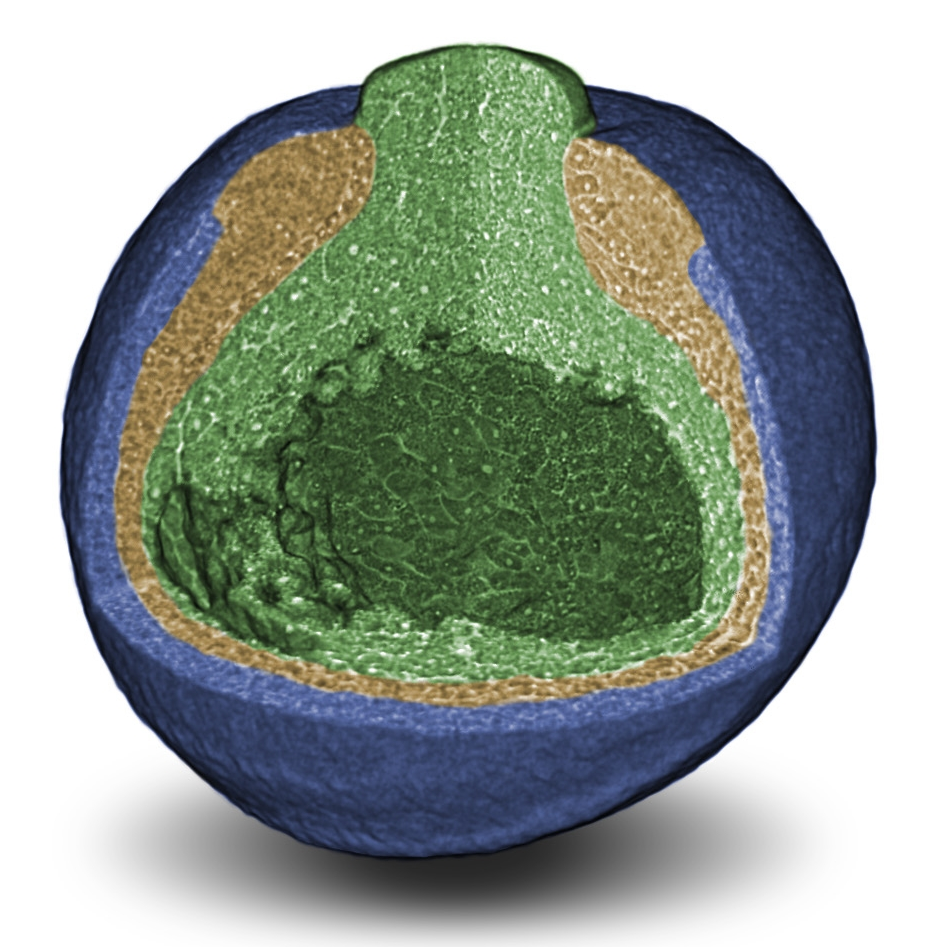
\includegraphics[height=\imh]{figures/title/seg.png}
\hfill 
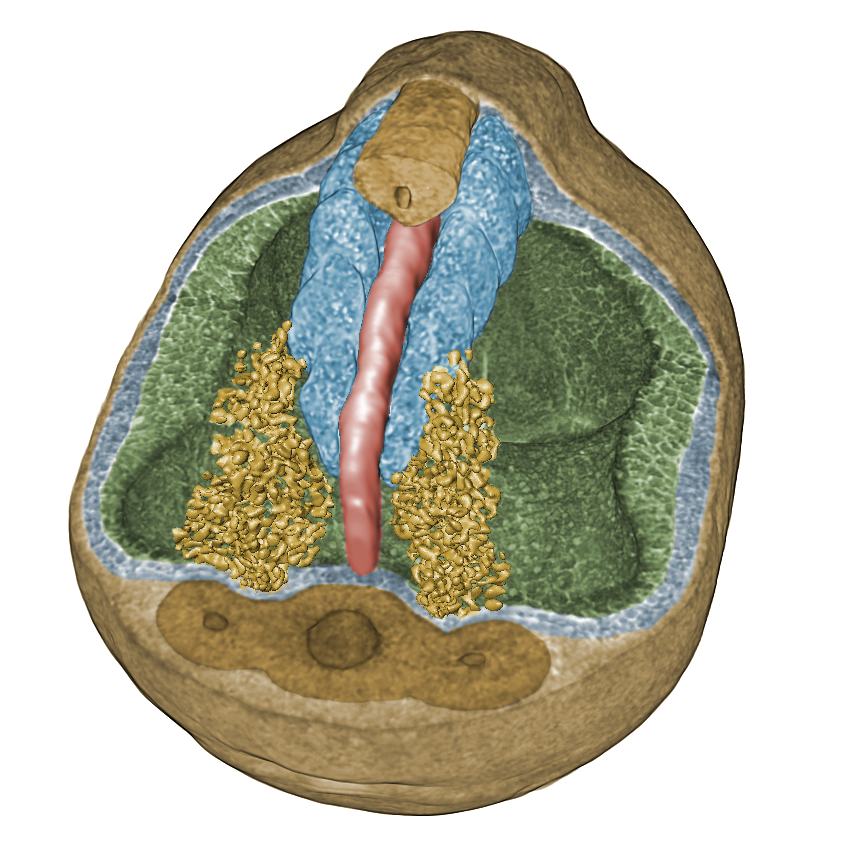
\includegraphics[height=\imh]{figures/title/neurula.png}
\hfill 
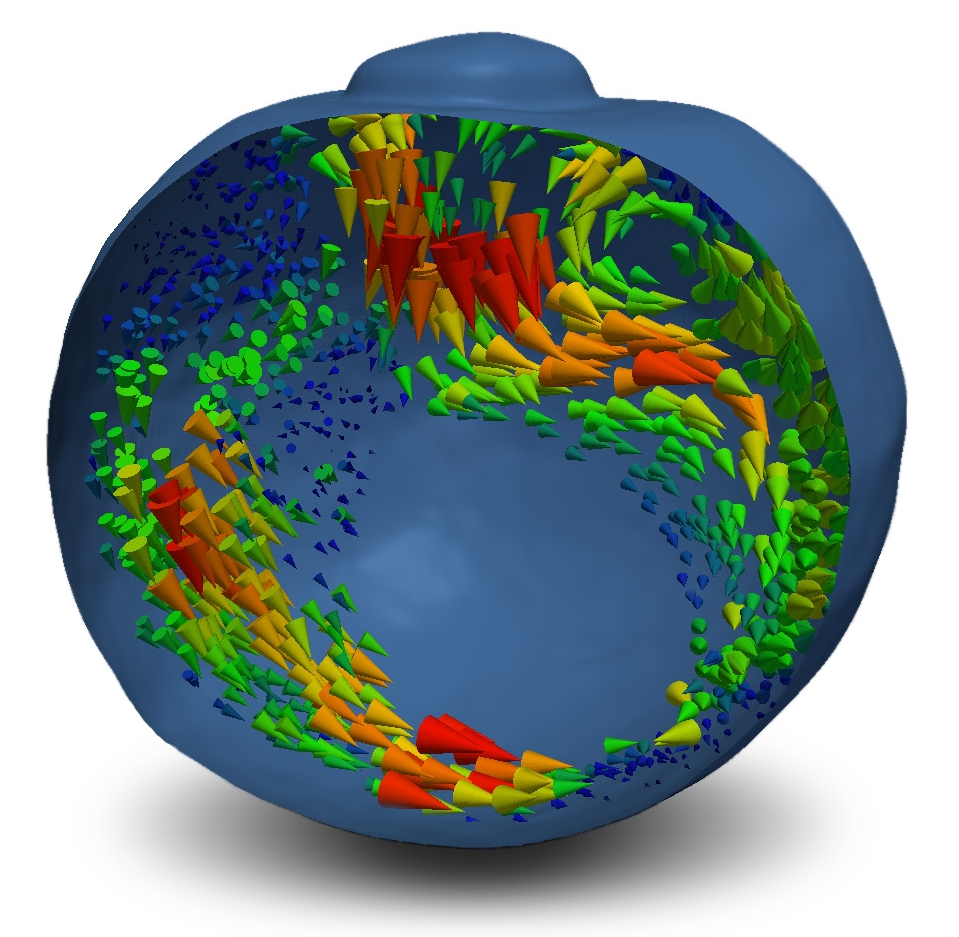
\includegraphics[height=\imh]{figures/title/flow.png}
}

\def\lh{1.1*\logoheight}
\addtobeamertemplate{title page}{%\hfill 
  
\includegraphics[height=\logoheight]{figures/logo/kth} \hfill 
  
\includegraphics[height=\logoheight]{figures/logo/kit} \hfill 
  
\includegraphics[height=0.85cm]{figures/logo/ssf} \hfill 
  
\includegraphics[height=\logoheight]{figures/logo/anka} \hfill 
  
\includegraphics[height=\logoheight]{figures/logo/anl} \hfill 
  
\includegraphics[height=\logoheight]{figures/logo/esrf} %\hfill 
}{}

%\AtBeginSection{\frame{\sectionpage}}
\AtBeginSubsection[]
{
  \begin{frame}[plain]{Outline}
    \tableofcontents[currentsection,currentsubsection]
  \end{frame}
} 

%%%%%%%%%%%%%%%%%%%%%%%%%%%%%%%%%%%%%%%%%%%%%%%%%%%%%%%%%%%%%%%%%%%%%%
%% BEGIN DOCUMENT
%%%%%%%%%%%%%%%%%%%%%%%%%%%%%%%%%%%%%%%%%%%%%%%%%%%%%%%%%%%%%%%%%%%%%%
\begin{document}
\selectlanguage{british}

%%%%%%%%%%%%%%%%%%%%%%%%%%%%%%%%%%%%%%%%%%%%%%%%%%%%%%%%%%%%%%%%%%%%%%
%% TITLE PAGE
\begin{frame}
  \titlepage
\end{frame}

%%%%%%%%%%%%%%%%%%%%%%%%%%%%%%%%%%%%%%%%%%%%%%%%%%%%%%%%%%%%%%%%%%%%%%
%% TABLE OF CONTENTS
\frame{
  \frametitle{Outline}
  \tableofcontents
}

%%%%%%%%%%%%%%%%%%%%%%%%%%%%%%%%%%%%%%%%%%%%%%%%%%%%%%%%%%%%%%%%%%%%%%
%%%%%%%%%%%%%%%%%%%%%%%%%%%%%%%%%%%%%%%%%%%%%%%%%%%%%%%%%%%%%%%%%%%%%%
\section{Propagation-based X-ray phase-contrast}
\subsection{Introduction to phase-contrast}

%%%%%%%%%%%%%%%%%%%%%%%%%%%%%%%%%%%%%%%%%%%%%%%%%%%%%%%%%%%%%%%%%%%%%%
\begin{frame} 
  \frametitle{Introduction}
  \begin{columns}
    \column{0.55\textwidth}
    \begin{itemize}
    \item Hard X-rays are strongly penetrating electromagnetic waves
    \item Interaction of X-ray and matter described by refractive index
    \begin{equation*}
      n = 1 - \delta + \ii \beta
    \end{equation*} 
  \end{itemize}
  \column{0.45\textwidth}
  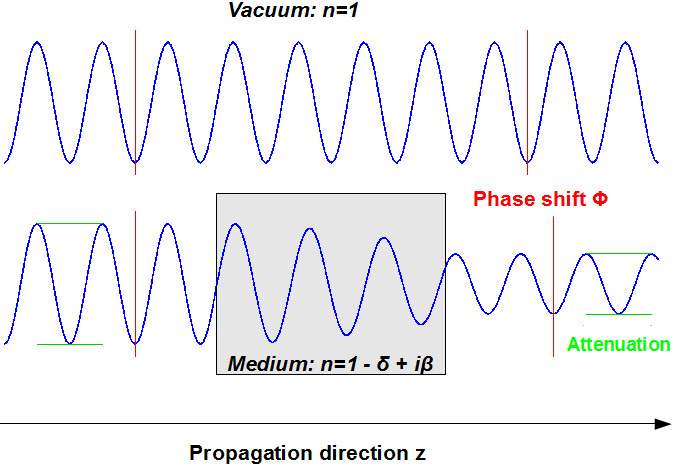
\includegraphics[width=\textwidth]{figures/interaction}
  \end{columns}
  \begin{itemize}
  \item  Transmitted wave front:   $\Psi_0=\sqrt{I_0}\expp{\ii\phi_0}$ 
   \item Absorption: destructive 
     \begin{equation*}
       \sqrt{I_0}=\sqrt{I_{\mathrm{in}}}\tfrac{2\pi}{\lambda}\int\Intd{z}\beta(z)
     \end{equation*}
   \item Phase: sensitive to soft-tissues
     \begin{equation*}
       \phi_0=\tfrac{2\pi}{\lambda}\int\Intd{z}\delta(z)
     \end{equation*}
   \end{itemize}
 \end{frame}

%%%%%%%%%%%%%%%%%%%%%%%%%%%%%%%%%%%%%%%%%%%%%%%%%%%%%%%%%%%%%%%%%%%%%%
\begin{frame}
  \frametitle{Introduction}
  \begin{itemize}
  \item Energy-dependence of refractive index
  \end{itemize}
  \centering
  \psfragfig[width=0.5\textwidth,height=0.4\textheight]
  {figures/refractive-index/fig-ratio}
  { %\footnotesize
      \psfrag{Energy}[c][c]{\scriptsize Energy $E$ [\si{eV}]}
      \psfrag{ratio}[c][r]{\scriptsize Ratio $\delta / \beta$}
      \psfrag{iron}{\tiny Fe}
      \psfrag{calcium}{\tiny Ca}
      \psfrag{silicon}{\tiny Si}
      \psfrag{carbon}{\tiny C}
      \psfrag{waterwater}{\tiny H$_2$O}
    }
    \begin{itemize}
    \item Use monochromatic coherent X-ray with energies s.t.
      \begin{equation*} 
      \frac{\delta}{\beta} \gg 1
    \end{equation*}
\item Phase-contrast imaging of weakly absorbing materials
  \end{itemize}
\end{frame}

%%%%%%%%%%%%%%%%%%%%%%%%%%%%%%%%%%%%%%%%%%%%%%%%%%%%%%%%%%%%%%%%%%%%%%
\begin{frame}
  \frametitle{Propagation-based phase contrast}
  \begin{columns}
    \column{0.5\textwidth}
    \begin{itemize}
    \item Simple setup: no additional optics, no scanning, no stepping
      \begin{itemize}
      \item \normalsize{stable, fast, efficient}
      \end{itemize}
    \item Intensity contrast emerges via free-space propagation of
      transmitted wave field
    \end{itemize}
    \column{0.5\textwidth}
      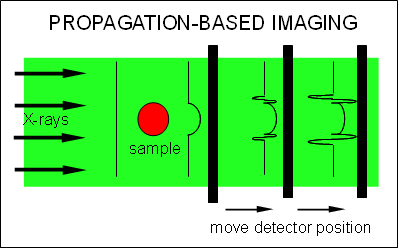
\includegraphics[
      width=\textwidth
      ]{figures/setup/propagation-based-imaging.png}
  \end{columns}
  \vspace{0.5cm}
  Sequence of intensity maps $I_z$: signal increases with $z$
  \begin{tikzpicture}[]
    \def\xx{0.25\textwidth};
    \def\picheight{0.18\textwidth};
    \small
    \node[inner sep=0pt,rotate=90,above] at (-\xx/2,\xx/2.5){Xenopus};
    % 5 cm    
    \node[inner sep=1pt,above] at (0,0){
      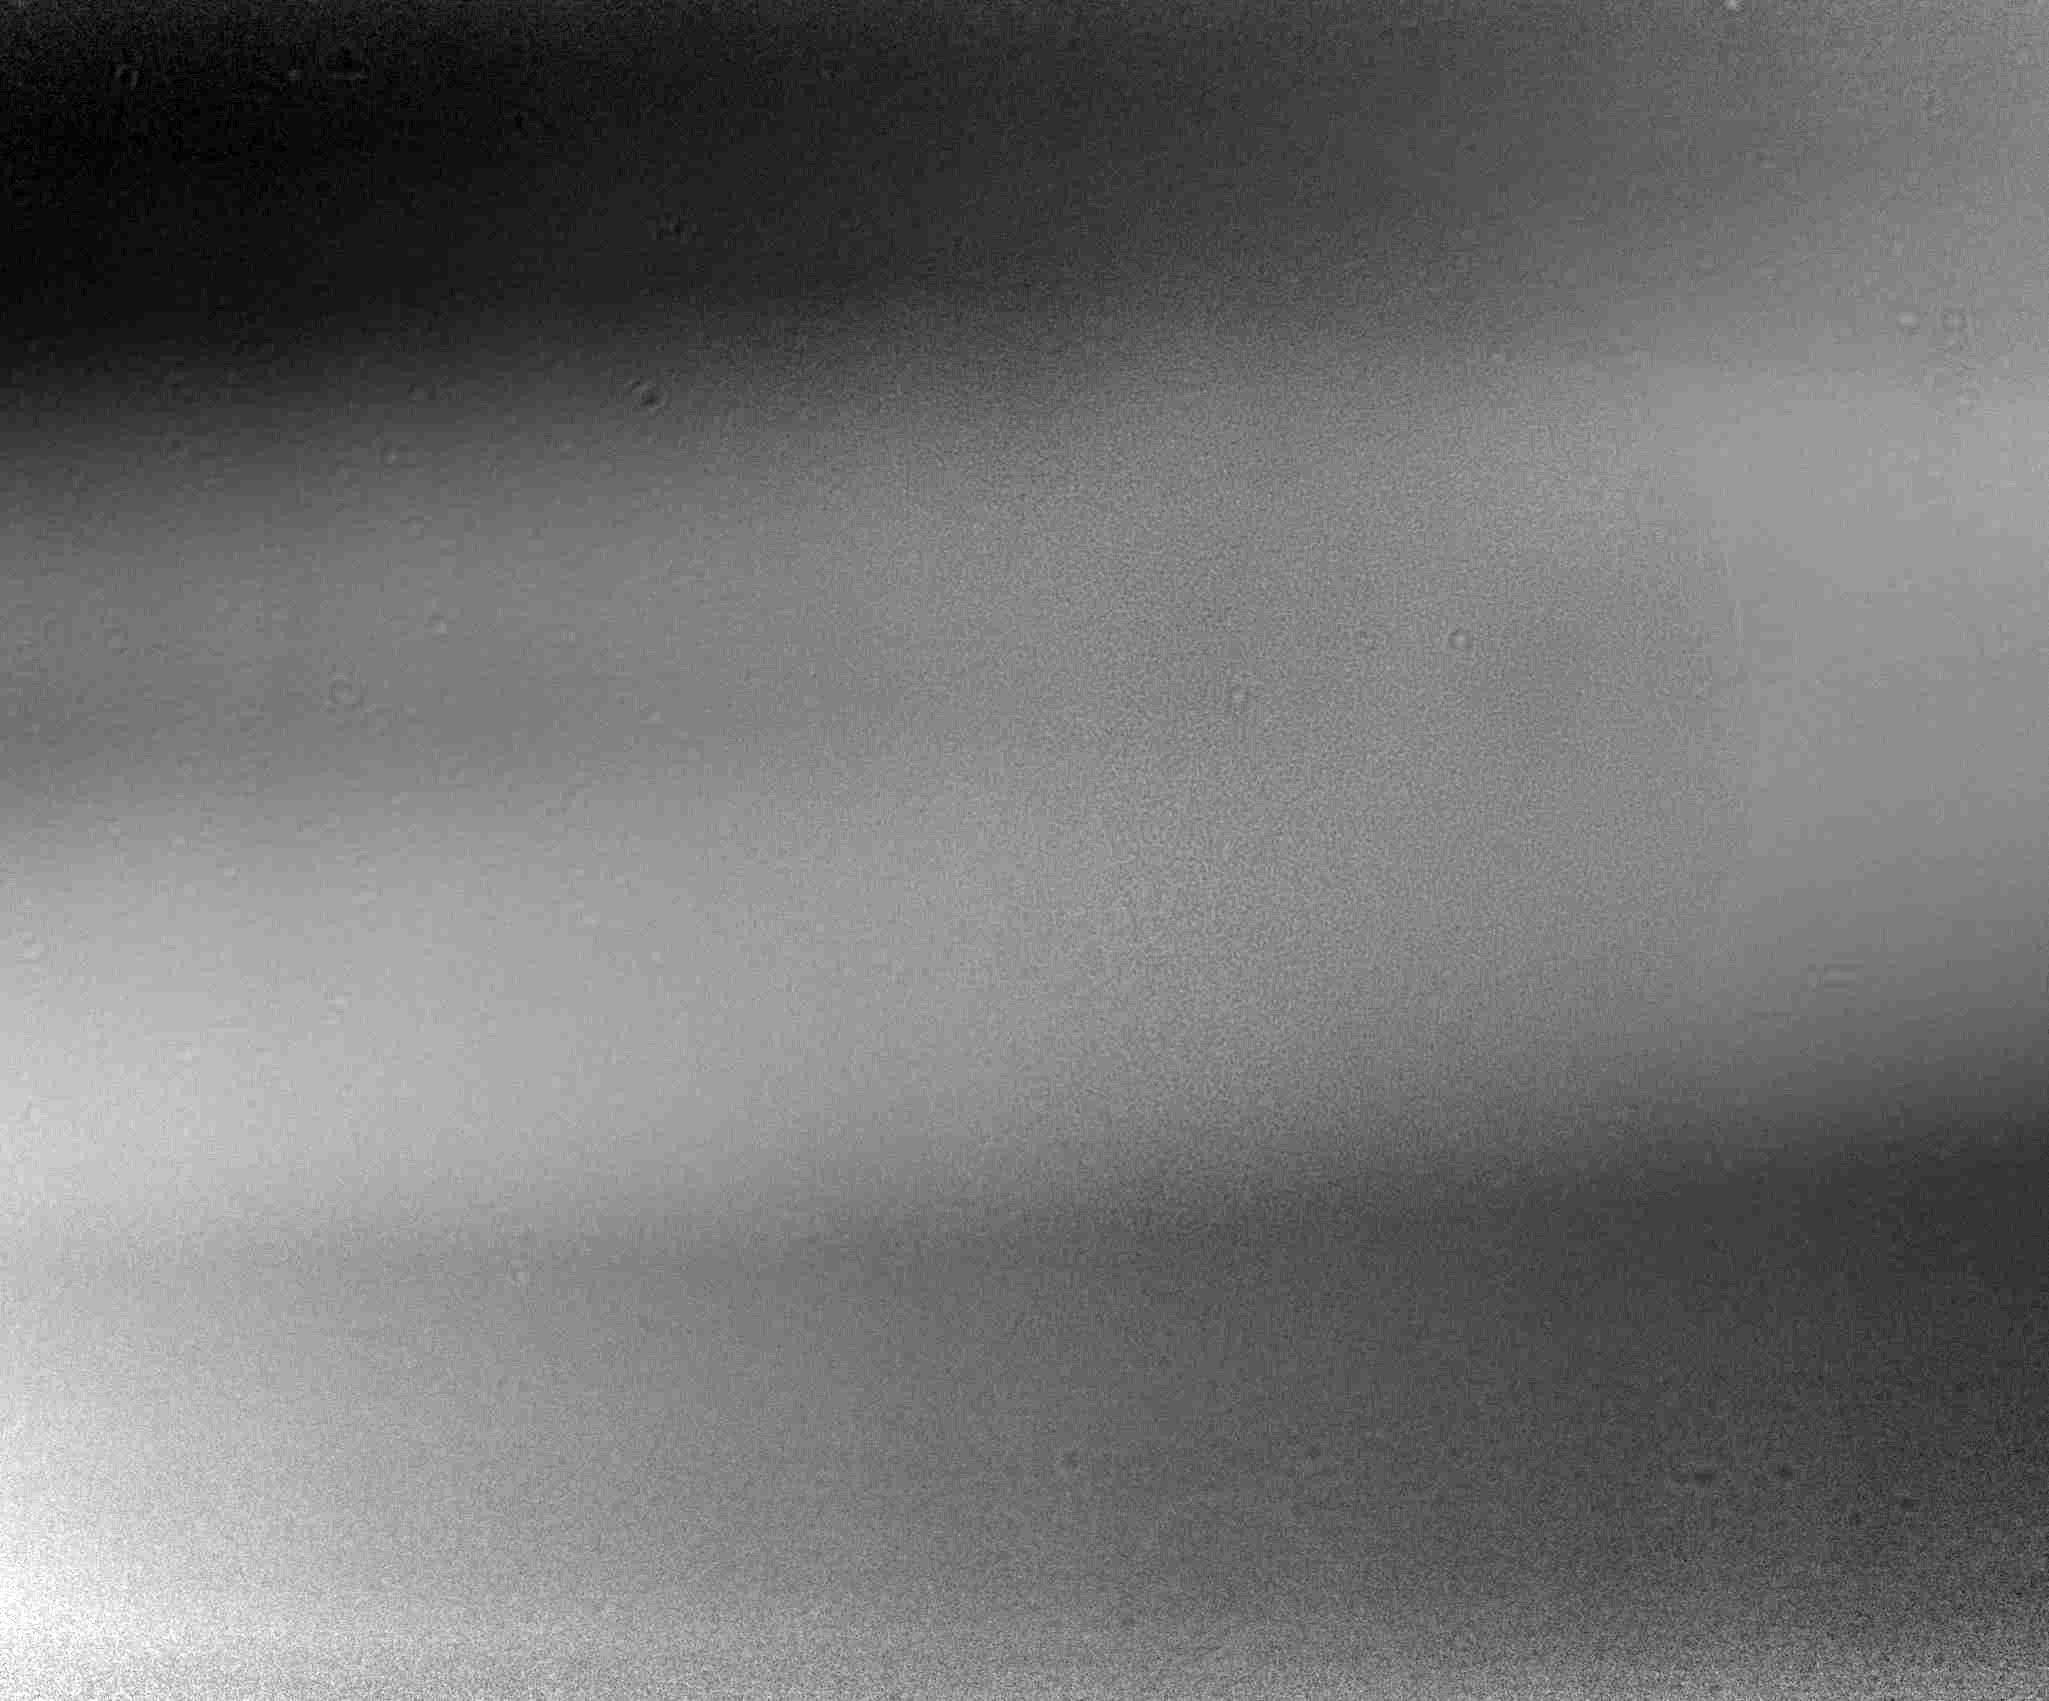
\includegraphics[height=\picheight]{figures/IntensitySequenceANKA/int0005mm.png}};         
    \node[inner sep=1pt,below] at (0,0){$\SI{0.5}{cm}$};
    % 18 cm    
    \node[inner sep=1pt,above] at (\xx,0){
      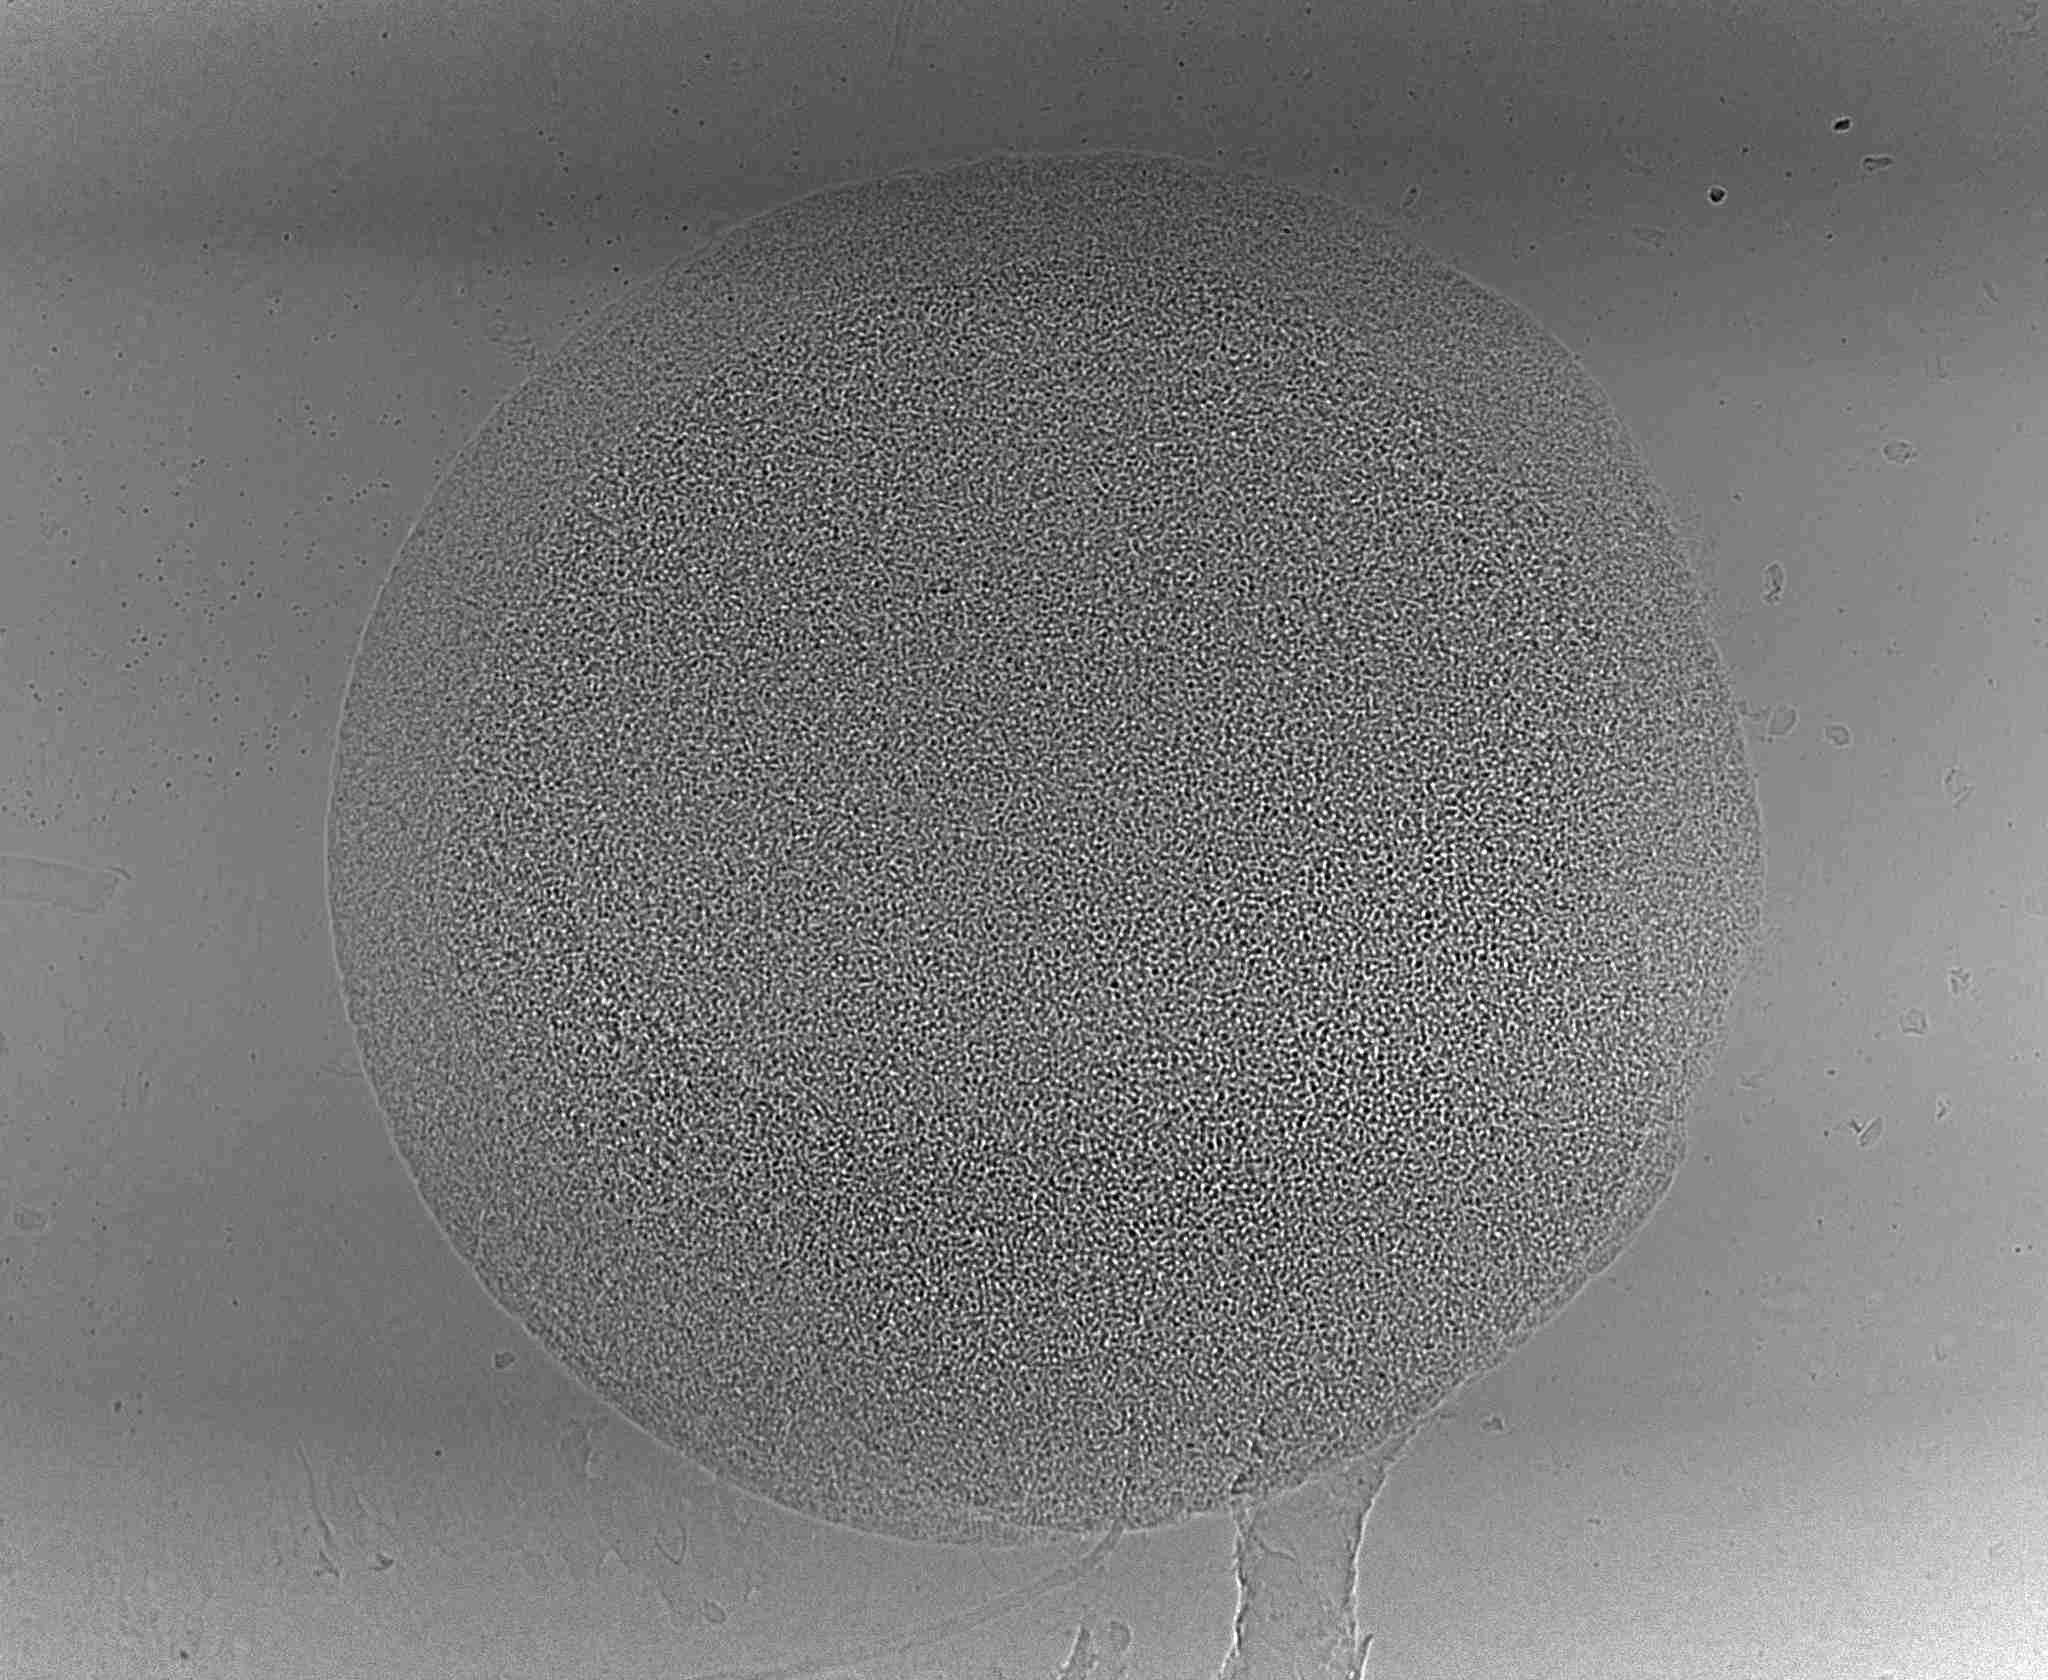
\includegraphics[height=\picheight]{figures/IntensitySequenceANKA/int0180mm.png}};         
    \node[inner sep=1pt,below] at (\xx,0){$\SI{18}{cm}$};
    % 58 cm    
    \node[inner sep=1pt,above] at (2*\xx,0){
      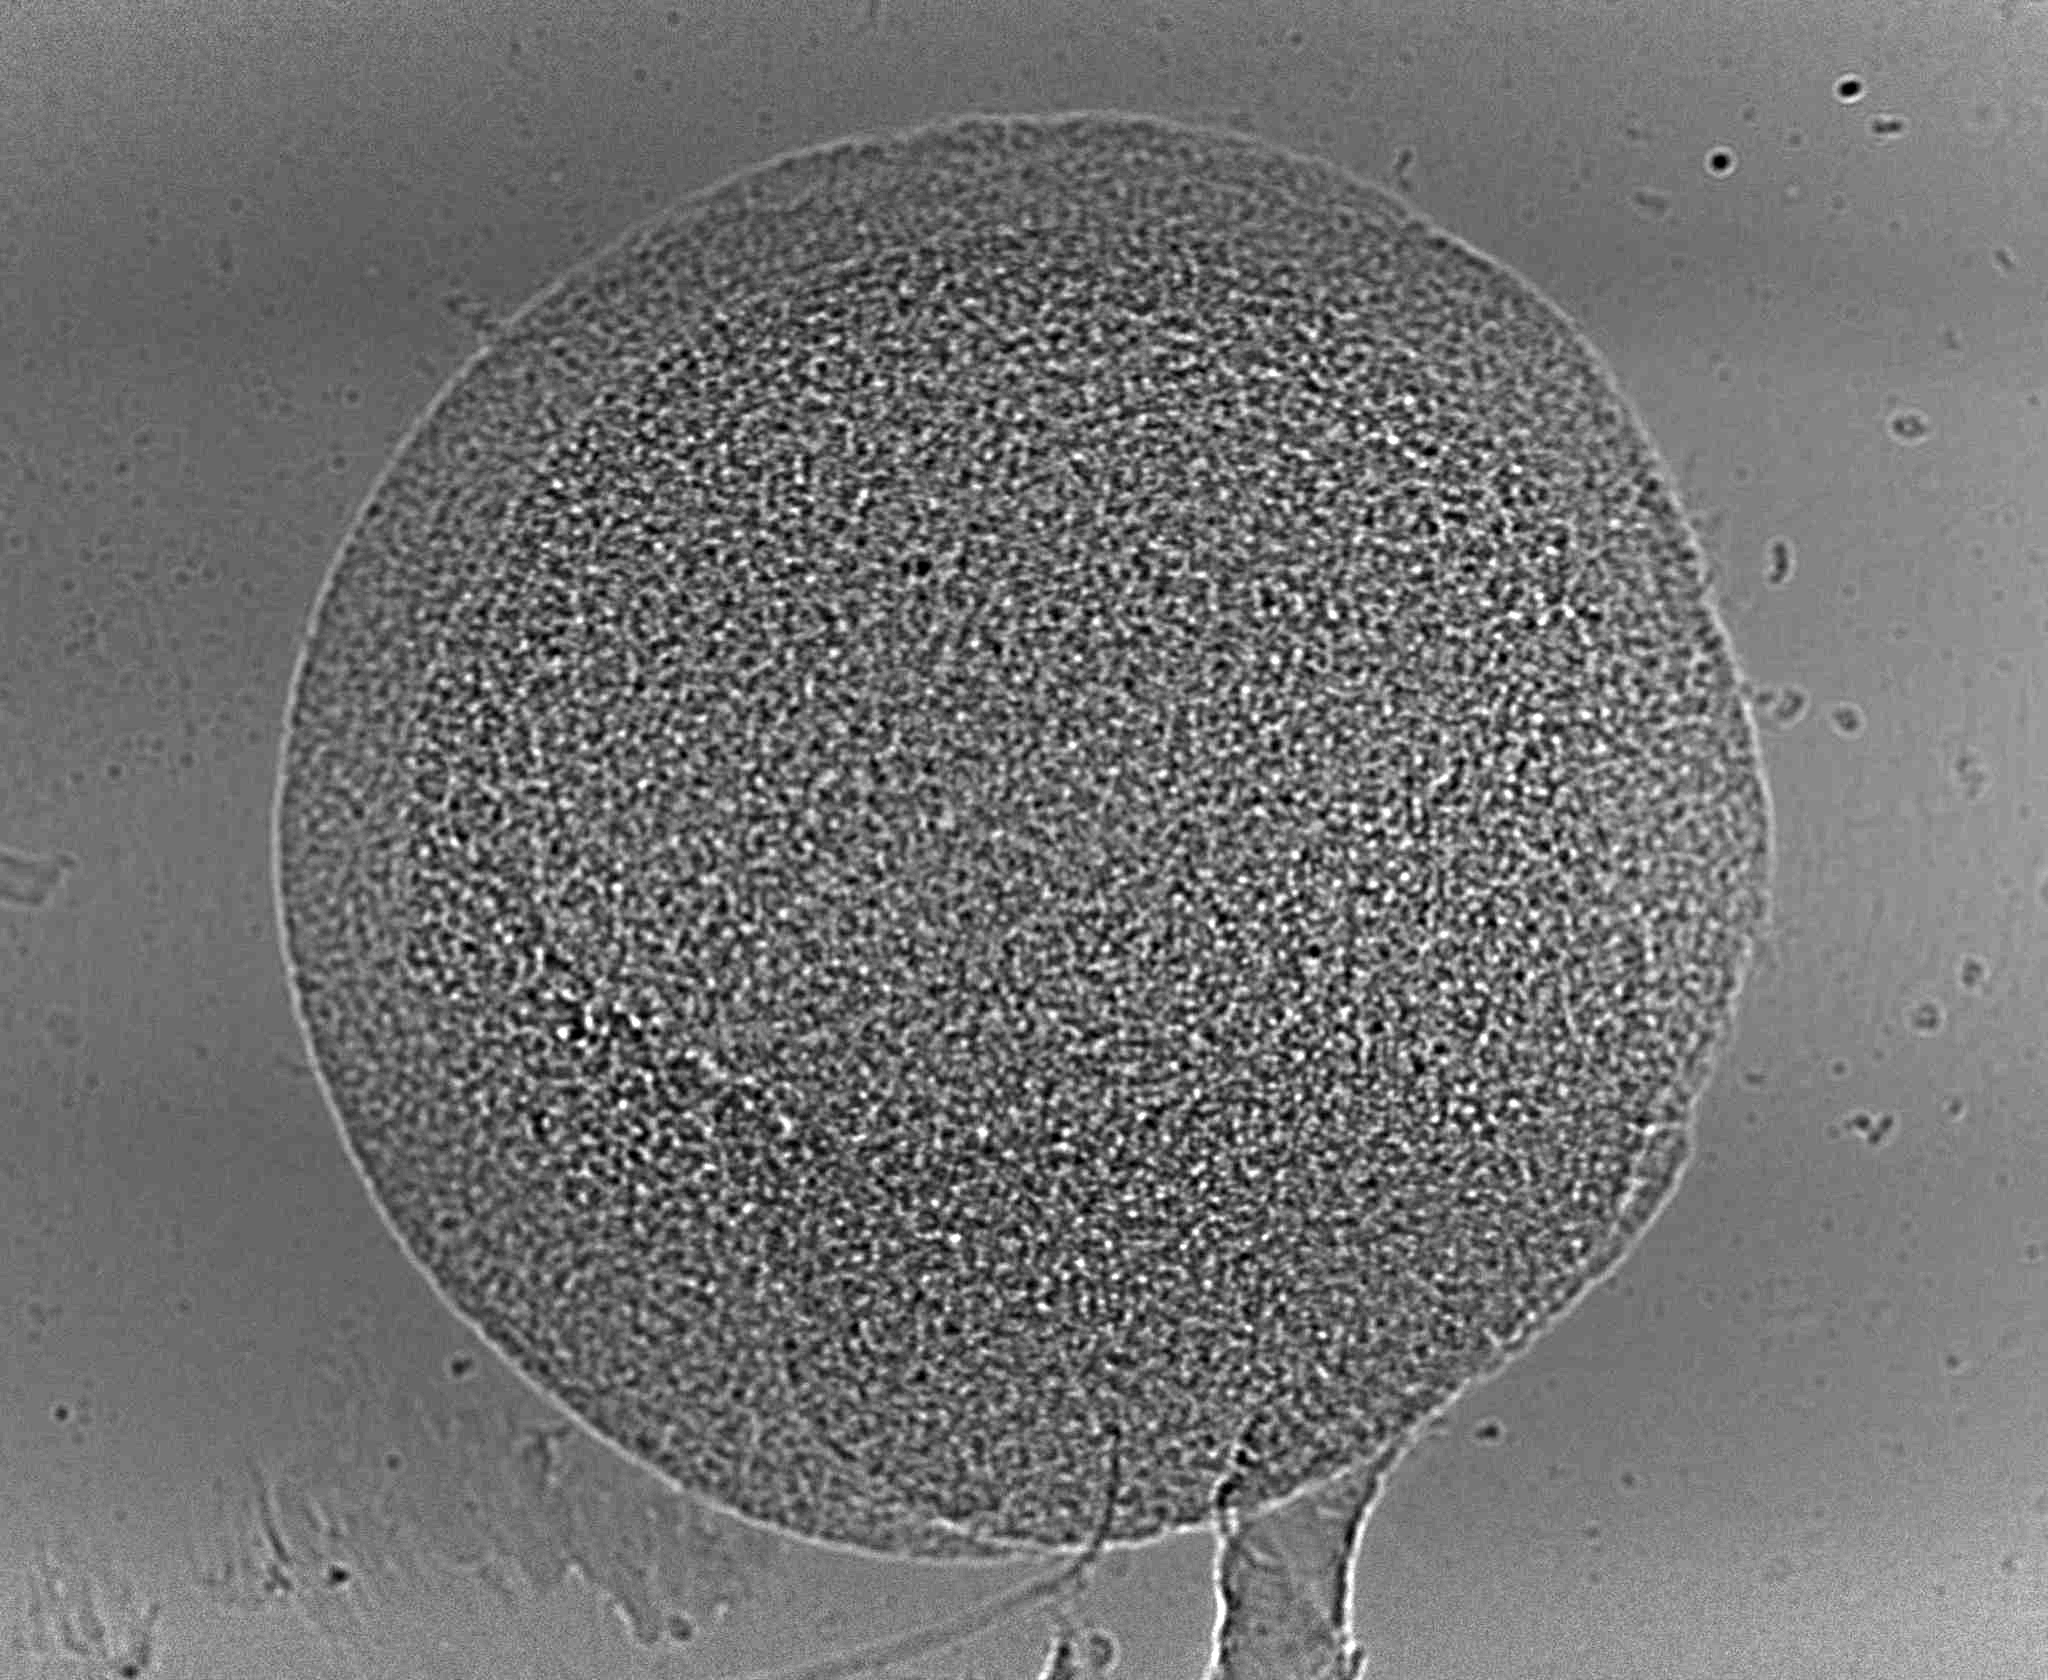
\includegraphics[height=\picheight]{figures/IntensitySequenceANKA/int0580mm.png}};         
    \node[inner sep=1pt,below] at (2*\xx,0){$\SI{58}{cm}$};
    % 108 cm    
    \node[inner sep=1pt,above] at (3*\xx,0){
      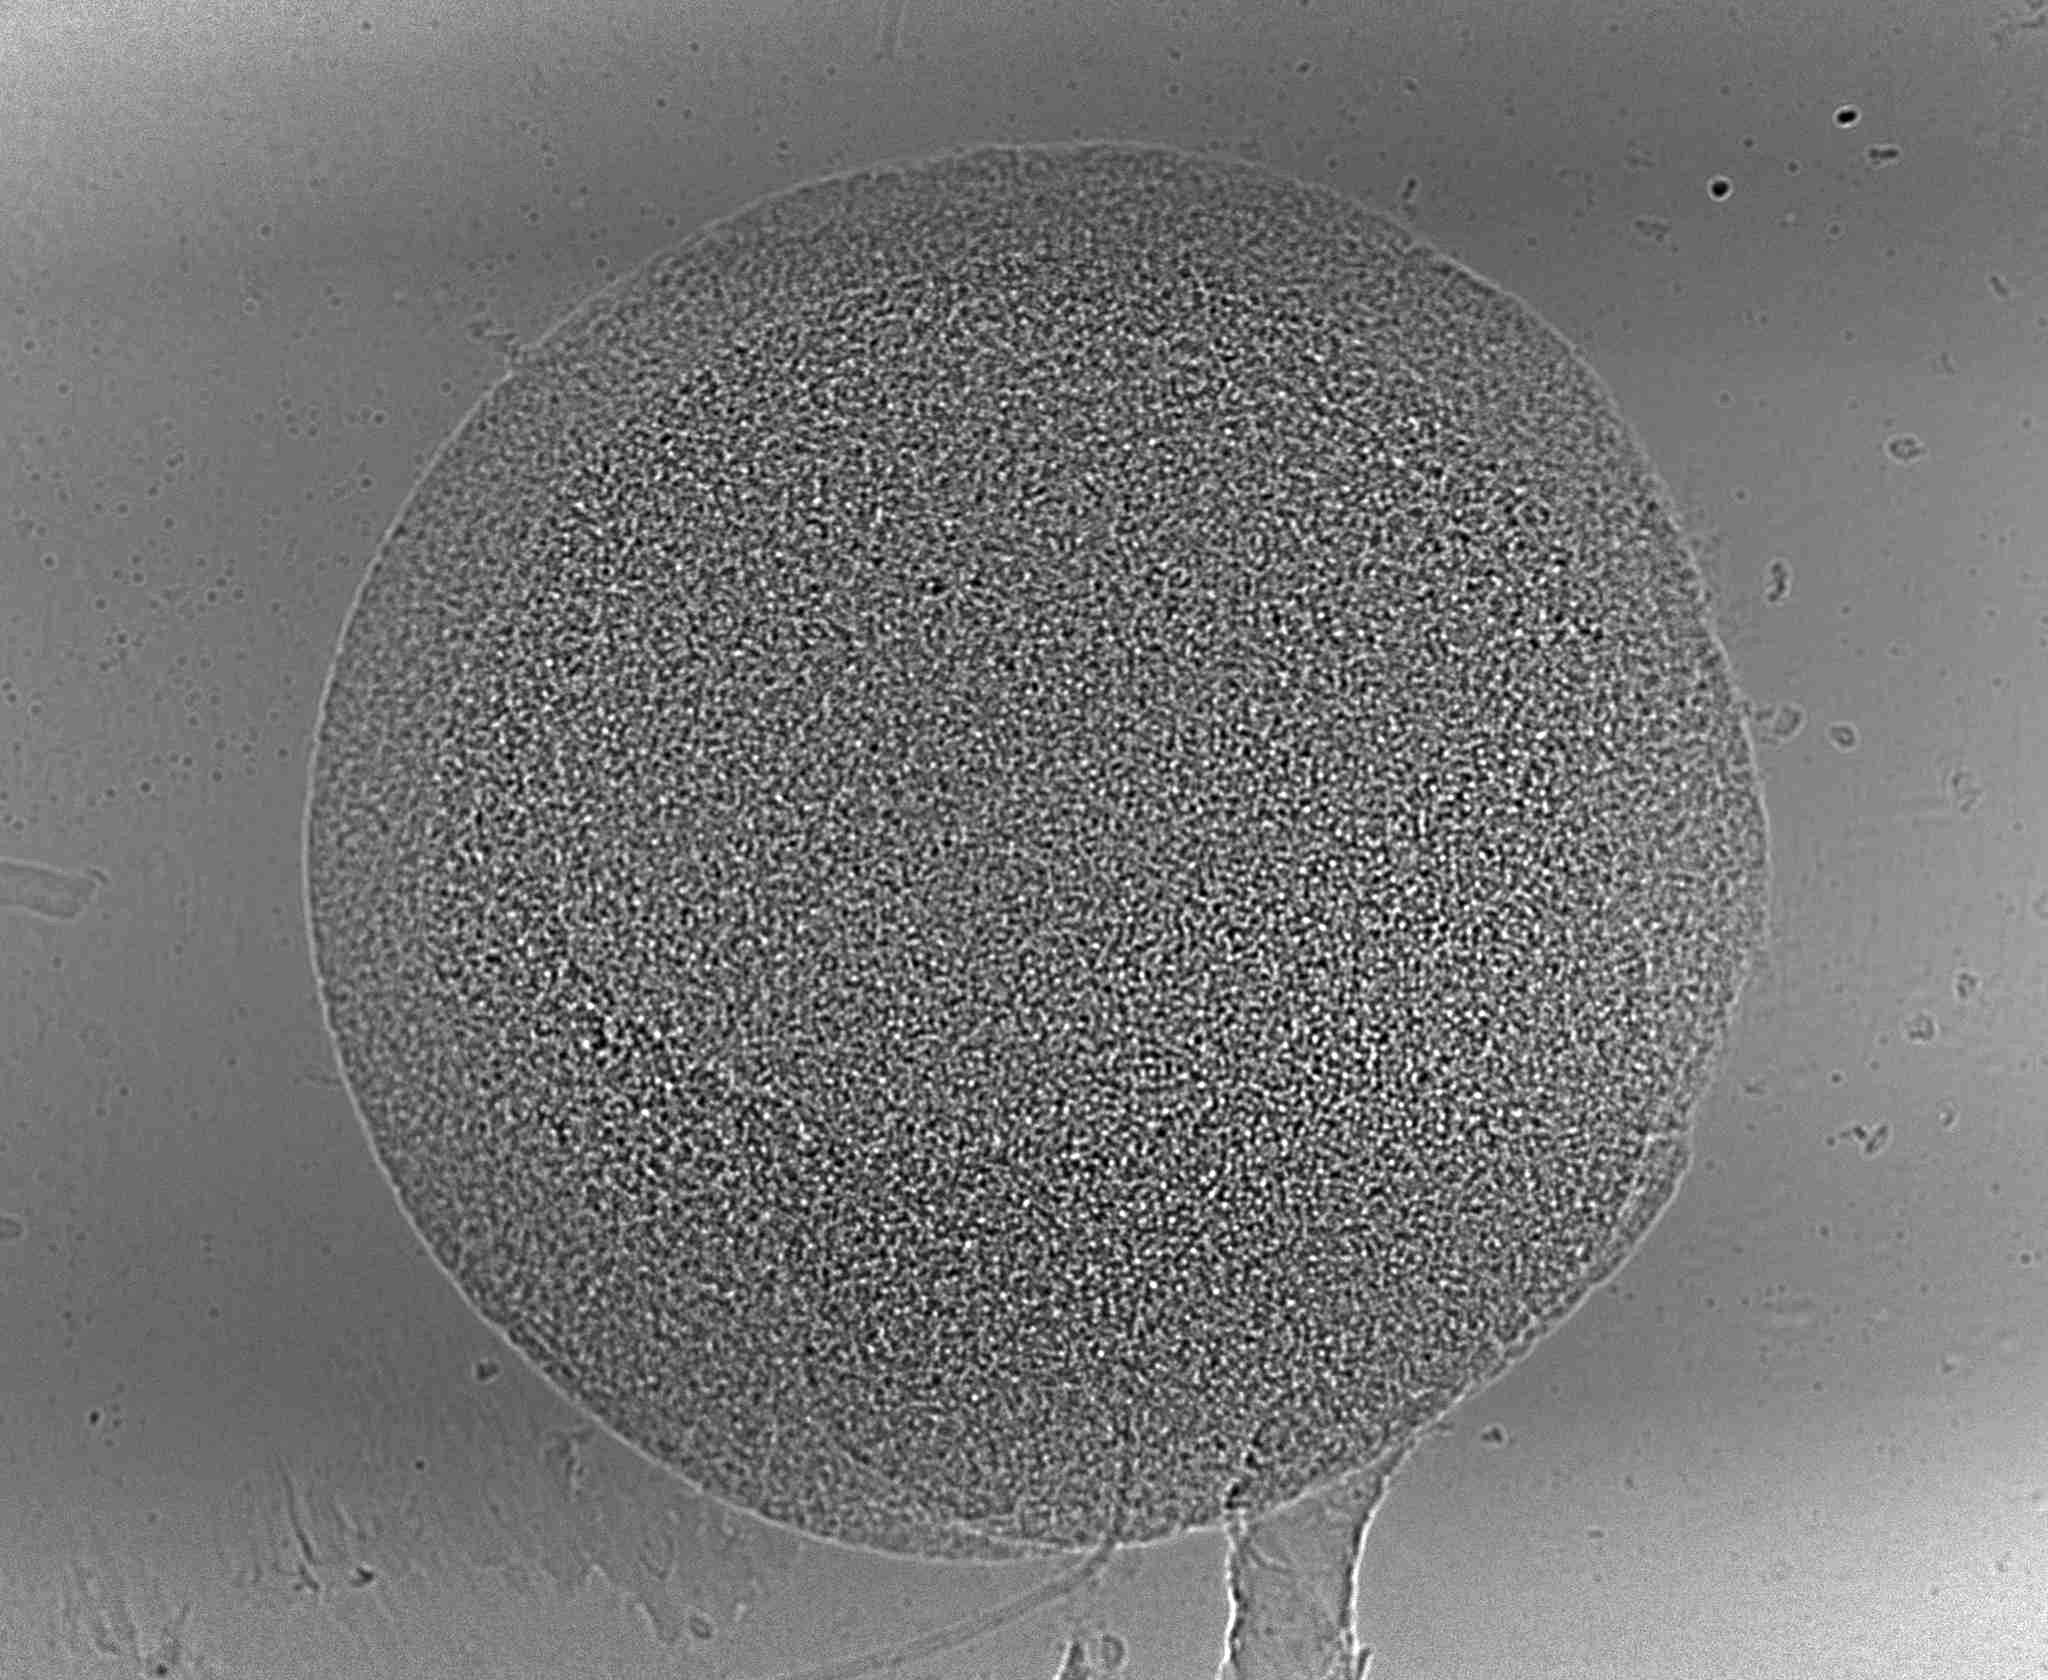
\includegraphics[height=\picheight]{figures/IntensitySequenceANKA/int1080mm.png}};         
    \node[inner sep=1pt,below] at (3*\xx,0){$\SI{108}{cm}$};
    \draw[very thick,->] (-0.5*\xx,-0.4) 
    node[below right]{object-detector distance $z$} 
    -- (3.5*\xx,-0.4);
    \end{tikzpicture}
\end{frame}

%%%%%%%%%%%%%%%%%%%%%%%%%%%%%%%%%%%%%%%%%%%%%%%%%%%%%%%%%%%%%%%%%%%%%%
\subsection{Experimental setup}
\label{sec:setup}

%%%%%%%%%%%%%%%%%%%%%%%%%%%%%%%%%%%%%%%%%%%%%%%%%%%%%%%%%%%%%%%%%%%%%%
\begin{frame}
  \frametitle{X-ray source}
  Synchrotron radiation is required
  \begin{itemize}
    \item High flux
    \begin{itemize}
    \item High spatial resolution
    \item Fast acquisition: image fast cell movement, high throughput
    \end{itemize}
  \item Coherence
    \begin{itemize}
    \item propagation-base phase-contrast
    \end{itemize}
    \item Quasimonochromatic spectrum (single harmonic or  monochromator)
    \begin{itemize}
    \item Reduce dose
    \item Propagation-base phase-contrast
    \end{itemize}
  \end{itemize}
  \vfill
  \centering
    \begin{tikzpicture}[]
      \node[] at (0,0){
        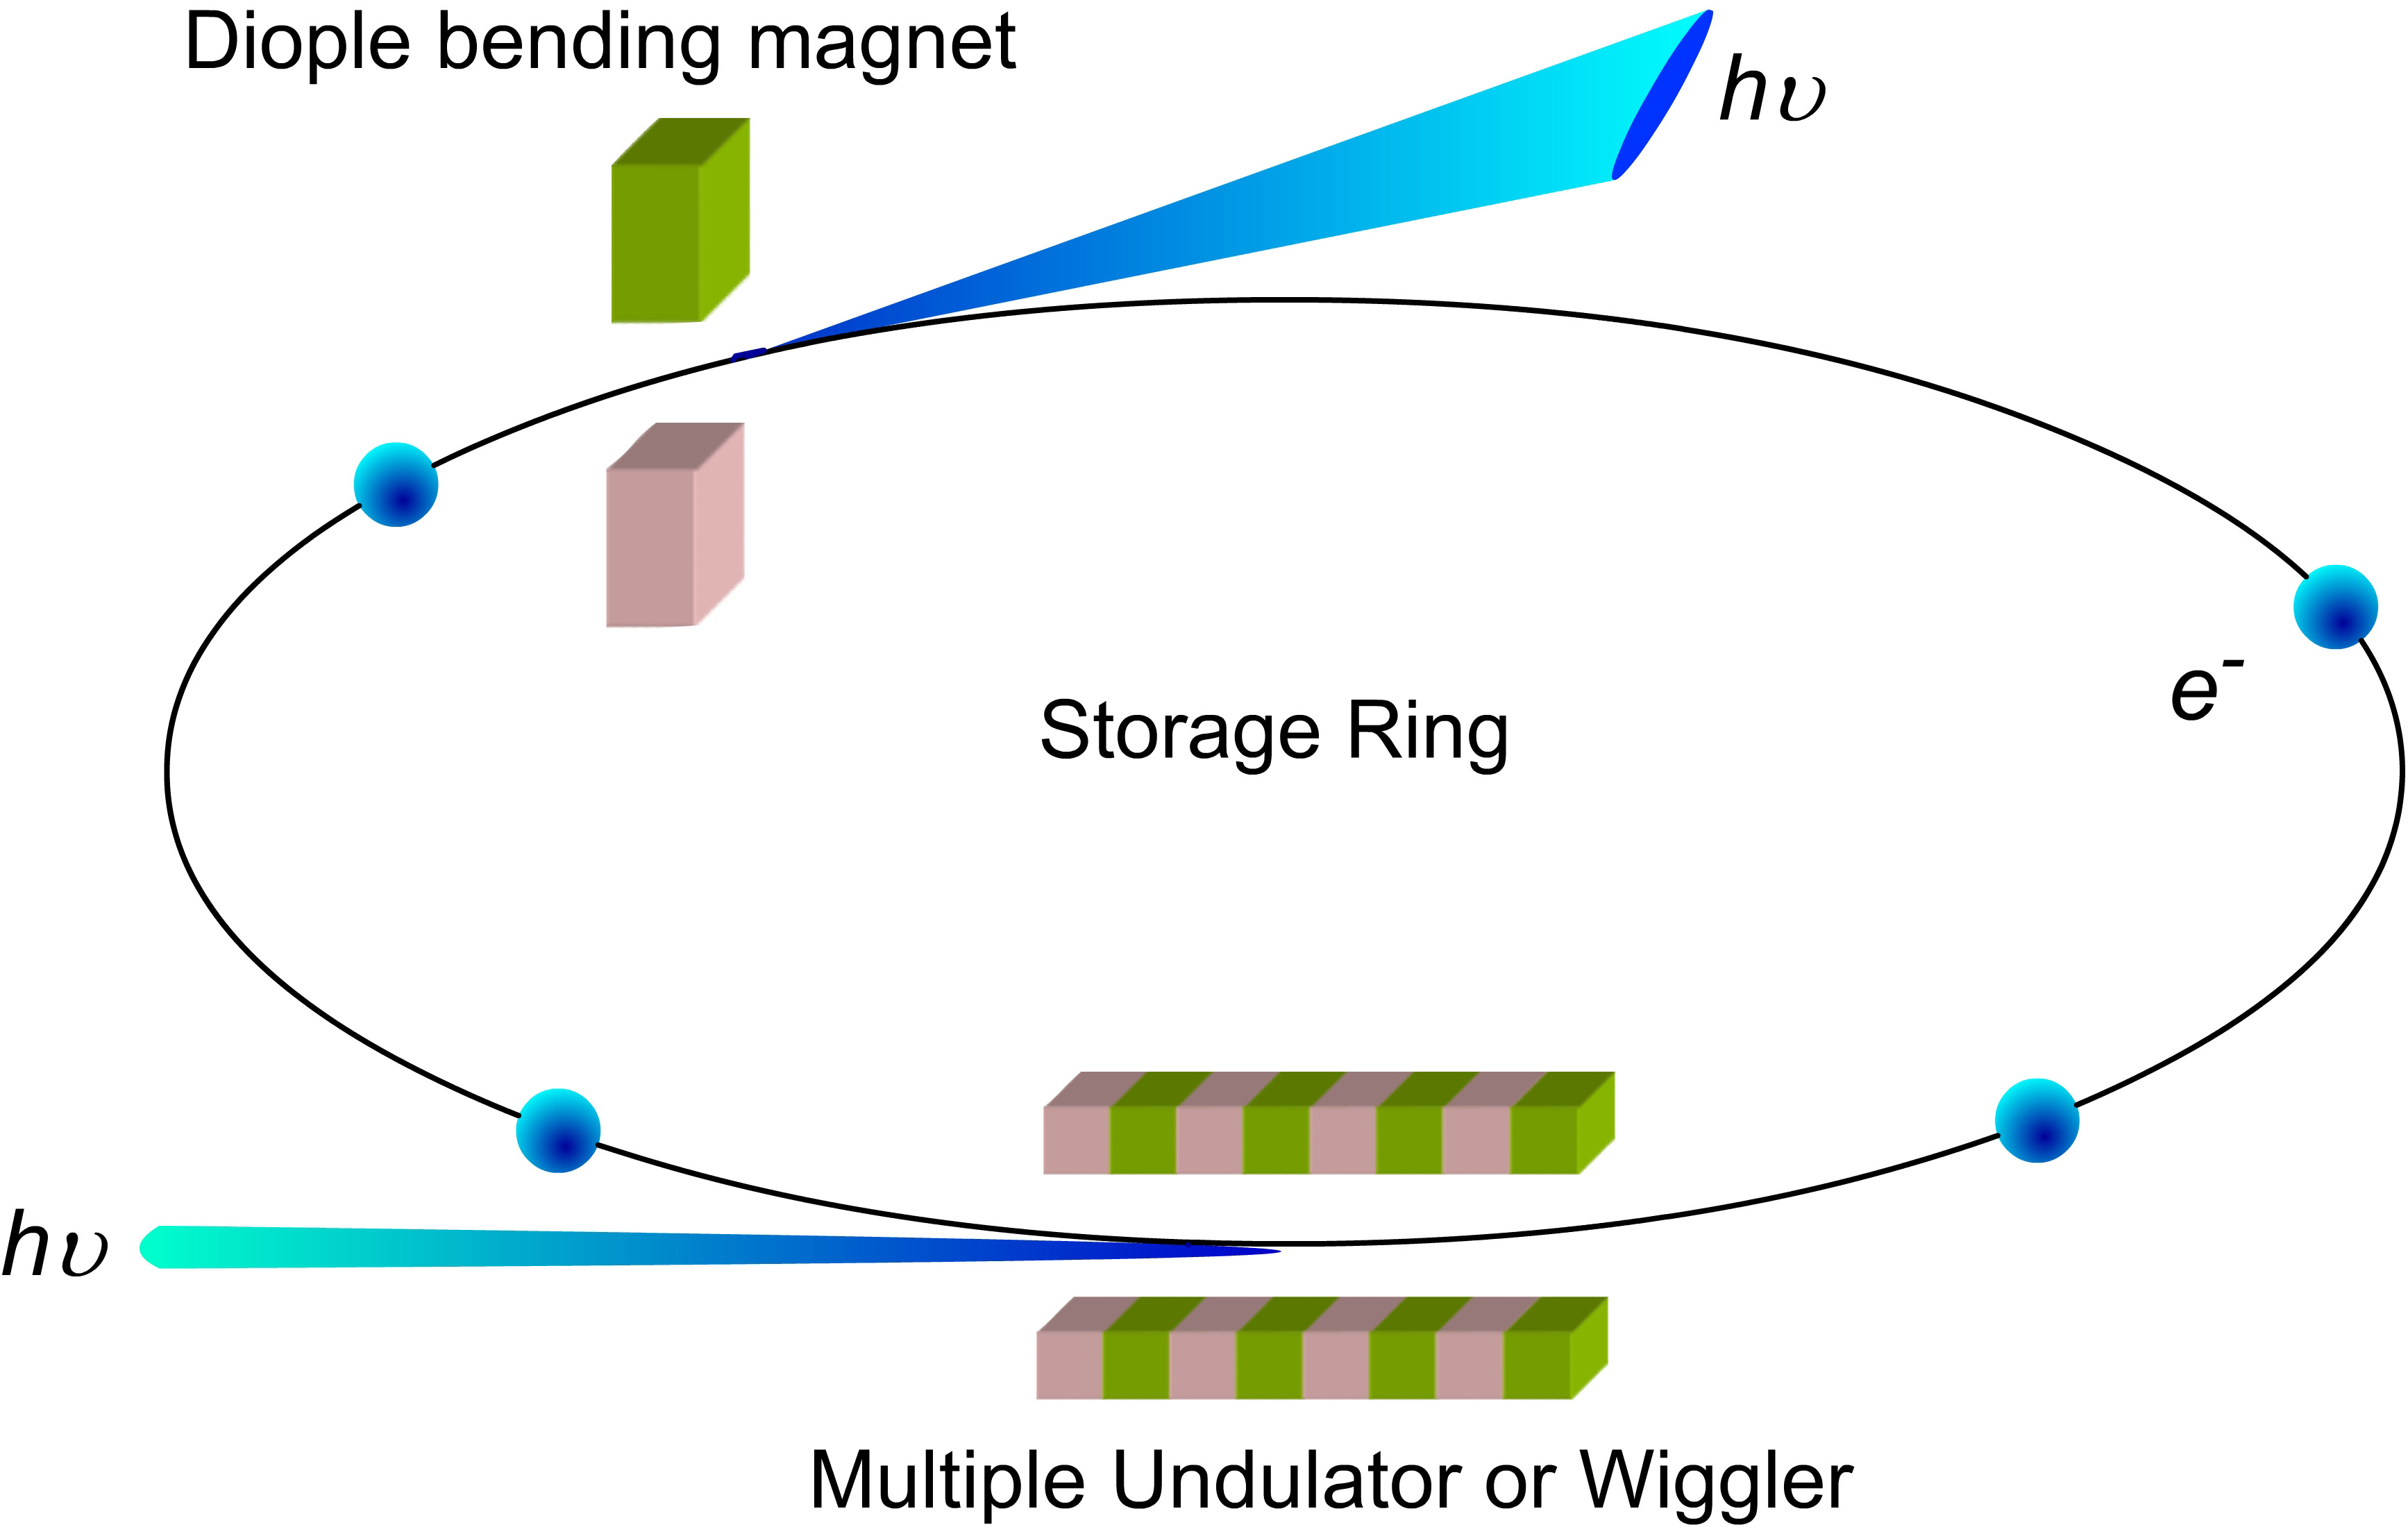
\includegraphics[height=0.3\textheight]{figures/synchrotron/schematic.jpg}};
    \end{tikzpicture}
\end{frame}


%%%%%%%%%%%%%%%%%%%%%%%%%%%%%%%%%%%%%%%%%%%%%%%%%%%%%%%%%%%%%%%%%%%%%%
\begin{frame}
  \frametitle{Experimental setup}
      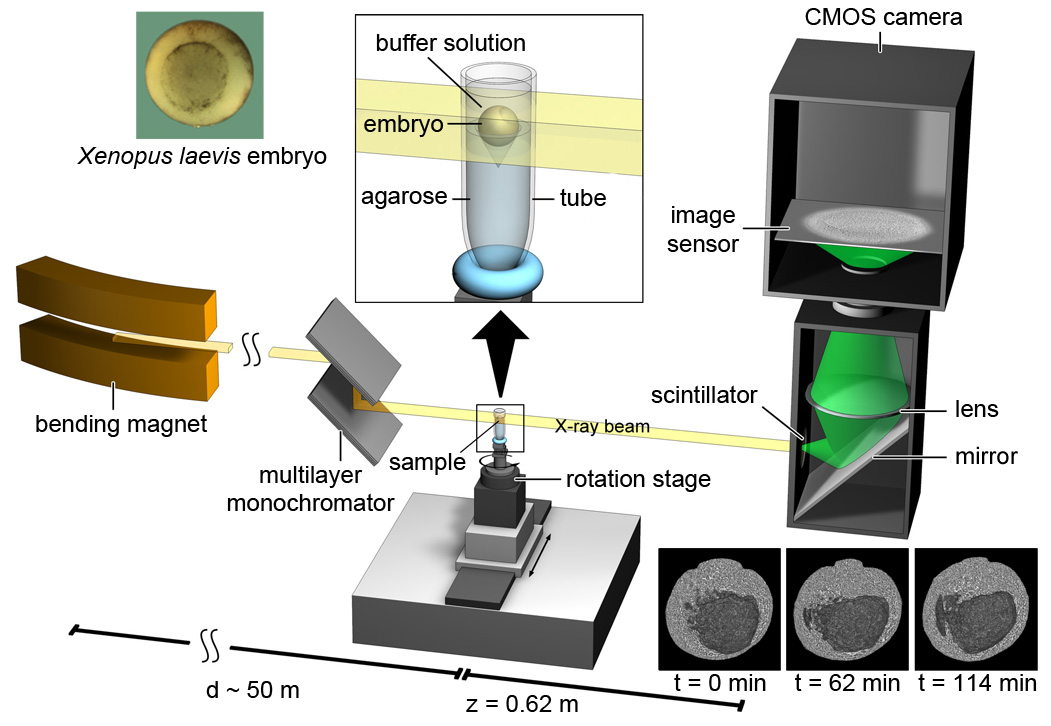
\includegraphics[width=1\textwidth]{figures/setup/setup.jpg}
\end{frame}



%%%%%%%%%%%%%%%%%%%%%%%%%%%%%%%%%%%%%%%%%%%%%%%%%%%%%%%%%%%%%%%%%%%%%%
%%%%%%%%%%%%%%%%%%%%%%%%%%%%%%%%%%%%%%%%%%%%%%%%%%%%%%%%%%%%%%%%%%%%%%
\subsection{Phase retrieval}
\label{sec:phase-retrieval}

%%%%%%%%%%%%%%%%%%%%%%%%%%%%%%%%%%%%%%%%%%%%%%%%%%%%%%%%%%%%%%%%%%%%%%
\begin{frame}
  \frametitle{Phase contrast}
  \begin{itemize}
  \item Rewrite Fresnel diffraction integral
    \begin{equation*}
    \F I_z(\vecxi) = 
    \int \Intd{\vecx}\exp{(-\ii 2\pi\vecx\cdot\vecxi)} 
    \Psi_0\left(\vecx-\tfrac{\lambda z}{2}\vecxi\right) 
    \Psi^*_0\left(\vecx+\tfrac{\lambda z}{2}\vecxi\right)
  \end{equation*}
  \flr{\small{$\F$: Fourier transform, $\vecx,\vecxi \in \R^2$\quad}\scriptsize{[Guigay 1977]}}
\item Intensity contrast $g_z=I_z/I_0-1$
  \item Expand exponential of exit wave field
    $\Psi_0=\sqrt{I_0}\expp{\ii\phi_0}$ 
    %=\sqrt{I_0}(1+\ii\phi_0-\phi_0^2+\order(\phi_0^3))
  \item Guigay up to $\order(\phi_0)$ (pure-phase object)
    \begin{equation*}
      \begin{split}
        &\F g_z(\vecxi) =
        2\sin(\pi\lambda z\vecxi^2)\F \phi_0(\vecxi) 
%        \quad \leftarrow \quad \mathrm{linear\;order}
        \\ & -\cos(\pi\lambda z\vecxi^2)\int\Intd{\vecxi'}
        \F\phi_0(\vecxi')\,\F\phi_0(\vecxi-\vecxi')
        \\ & +\expp{\ii\pi\lambda z\vecxi^2}\int\Intd{\vecxi'}
        \expp{-\ii 2\pi\lambda z\vecxi\cdot\vecxi'} 
        \F\phi_0(\vecxi')\,\F\phi_0(\vecxi-\vecxi')
%        \\ & +\order( ( \ft{\phi}_0 )^3 ) \;.
      \end{split}
    \end{equation*}
  \end{itemize}
\end{frame}

%%%%%%%%%%%%%%%%%%%%%%%%%%%%%%%%%%%%%%%%%%%%%%%%%%%%%%%%%%%%%%%%%%%%%%
\begin{frame}
  \frametitle{Phase contrast}

    Linear approximations

    % CTF
    \begin{itemize}
    \item Contrast transfer function (CTF)
      \begin{itemize}
      \item Weakly varying phase:
      $\abs{\phi_0(\vecx+\tfrac{\lambda z}{2}\vecxi)
        -\phi_0(\vecx-\tfrac{\lambda z}{2}\vecxi)}\ll 1$
    \end{itemize}

    \begin{equation*}
          \F g_z(\vecxi) = 2\sin(\pi\lambda z\vecxi^2) \F\phi_0(\vecxi)
        \end{equation*}
  \end{itemize}
  % TIE
  \vfill
  \begin{itemize}
  \item Linearised transport-of-intensity equation (TIE)
    \begin{itemize}
    \item Edge-enhancement regime: small propagation distance
    \end{itemize}

    \begin{equation*}
      \F g_z(\vecxi)  = 2\pi\lambda z\vecxi^2 \F\phi_0(\vecxi) 
    \end{equation*}
  \end{itemize}
  \vfill
  \begin{tikzpicture}[]
    \node[above] at (0,0){
      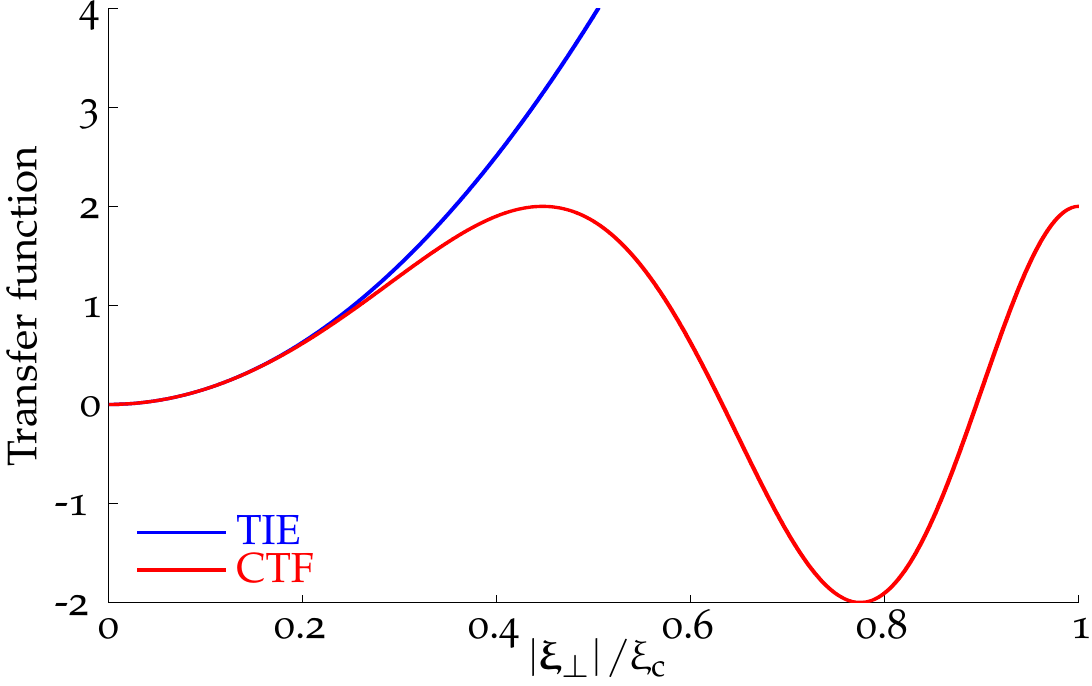
\includegraphics[height=0.35\textheight]{figures/contrast-transfer/contrast-transfer.png}};         
    \end{tikzpicture}
\end{frame}

%%%%%%%%%%%%%%%%%%%%%%%%%%%%%%%%%%%%%%%%%%%%%%%%%%%%%%%%%%%%%%%%%%%%%%
\begin{frame}
  \frametitle{Phase retrieval}
  Linear models

  \begin{columns}
    \column{0.6\textwidth}
    \begin{itemize}
    \item Contrast transfer function (CTF)
      \begin{itemize}
      \item High resolution
      \item Limited to weakly varying phases
      \end{itemize}
    \end{itemize}

    \begin{equation*}
      \F\phi_0(\vecxi) = \frac{\F g_z(\vecxi) }{2\sin(\pi\lambda z\vecxi^2)}
    \end{equation*}
    \reff{Guigay 1977; Gureyev et al. 2006; Cloetens 1998}
    \vfill
    \begin{itemize}
    \item Linearised TIE: Paganin phase retrieval
      \begin{itemize}
      \item Valid for small propagation distance
      \item Low-pass filter for large $z$
      \end{itemize}

      \begin{equation*}
        \F\phi_0(\vecxi) = \frac{\F g_z(\vecxi) }{2\pi\lambda z\vecxi^2}
      \end{equation*}
%     \reff{Teague 1982; Paganin \& Nugent 1998; Bronnikov 2003}
    \end{itemize}
    \column{0.5\textwidth}
    \begin{tikzpicture}[]
      \node[above] at (0,0){
        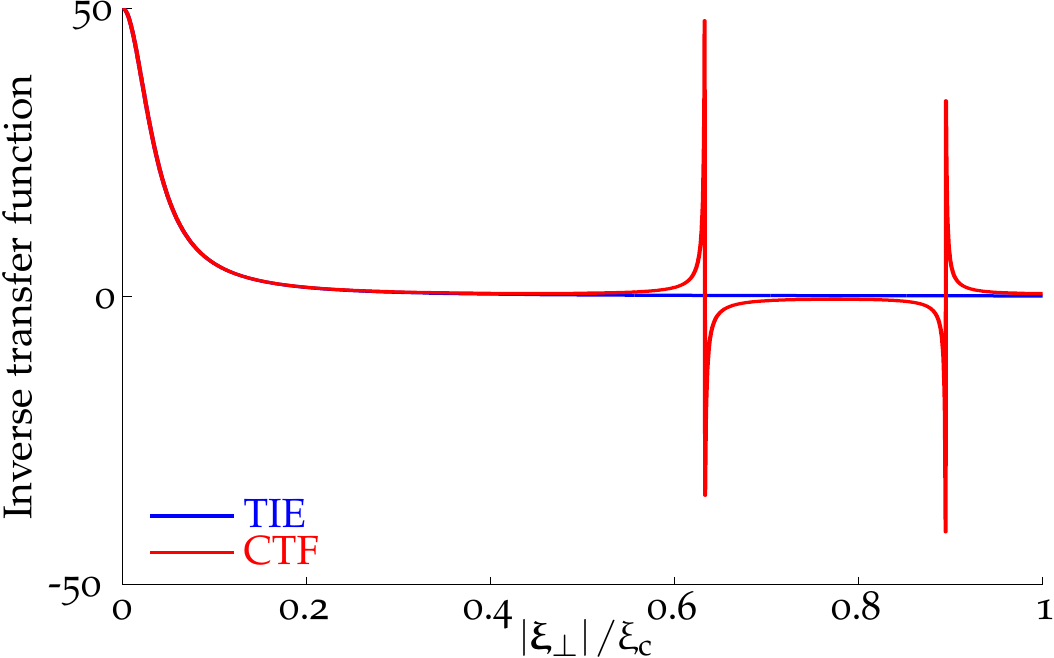
\includegraphics[height=0.4\textheight, width=\textwidth]
        {figures/contrast-transfer/inverse-transfer.png}};
    \end{tikzpicture}
  \end{columns}
\end{frame}

%%%%%%%%%%%%%%%%%%%%%%%%%%%%%%%%%%%%%%%%%%%%%%%%%%%%%%%%%%%%%%%%%%%%%%
\begin{frame}
  \frametitle{Phase retrieval}
  Problem
  \begin{itemize}
  \item Weak intensity contrast $g_z$ at small $z$
    \begin{itemize}
    \item Noise-to-signal in $I_z\propto\frac{1}{\sqrt{z}}$
    \item Noise in $\phi_0\propto\frac{1}{z}$
    \end{itemize}

    $\rar$ Measure at large $z$
  \item At large $z$: low resolution for Paganin phase retrieval

    $\rar$ CTF phase retrieval
  \item Extended objects (eg Xenopus embryos) exhibit phase variations
    of order $\order(\SI{1}{rad})$
  \item CTF phase retrieval fails (quasiperiodic artifacts)
  \end{itemize}

  What to do?  $\rar$ Phase retrieval beyond linear approximations
\end{frame}


%%%%%%%%%%%%%%%%%%%%%%%%%%%%%%%%%%%%%%%%%%%%%%%%%%%%%%%%%%%%%%%%%%%%%%
\begin{frame}
  \frametitle{Nonlinear phase retrieval}
  
  TIE beyond linearity
  \begin{itemize}
  \item Systematic expansion of $g_z$ and $\phi_z$ in powers of $z$
  \item Expansion coefficients determined full paraxial wave equation
    (TIE is the imaginary part of PWE)
  \item Nonlinear corrections to $\phi_0$:
    \begin{equation*}
      \begin{split}
        \np^2\phi_{0}&=-\frac{k}{z}g_z\\
        &+\frac{z}{2k}\left[
          \left(\nabla_\perp^2\phi_{0}\right)^2 +\tfrac12 \nabla_\perp^2
        \left(\nabla_\perp\phi_{0}\right)^2 +\left(\nabla_\perp
          \nabla_\perp^2 \phi_{0}\right) \cdot \nabla_\perp \phi_{0}
        \right] 
      \end{split}
    \end{equation*}
  \item Perturbation theory: evaluate correction in terms of leading
    order result (Paganin)
  \item $\rar$ Quantitative improvement of reconstructed phases
  \item But: low resolution due to leading order
  \end{itemize}
       \reff{Moosmann et al., Opt. Express 2010}

   What else? $\rar$ Consider contrast transfer function
\end{frame}



%%%%%%%%%%%%%%%%%%%%%%%%%%%%%%%%%%%%%%%%%%%%%%%%%%%%%%%%%%%%%%%%%%%%%%
\begin{frame}
  \frametitle{Evolution of intensity contrast}
  Examine contrast transfer from phase to intensity
  \begin{itemize}
  \item Compute intensity contrast from input phase map (Lena)
  \item Amplify phase variations by upscaling of input phase
  \item Consider Fourier transformed intensity as a
    function of phase upscaling
  \end{itemize}
  \begin{columns}
    %% LEFT: Movie
    \column{0.4\textwidth}
    \begin{tikzpicture}
      \def\imh{0.8\textwidth}
      \small
      \node[inner sep=1pt,above] at (0,0){
        \href{run:videos/intensity/FT-intensity_vs_distance.avi?autostart&loop}{
          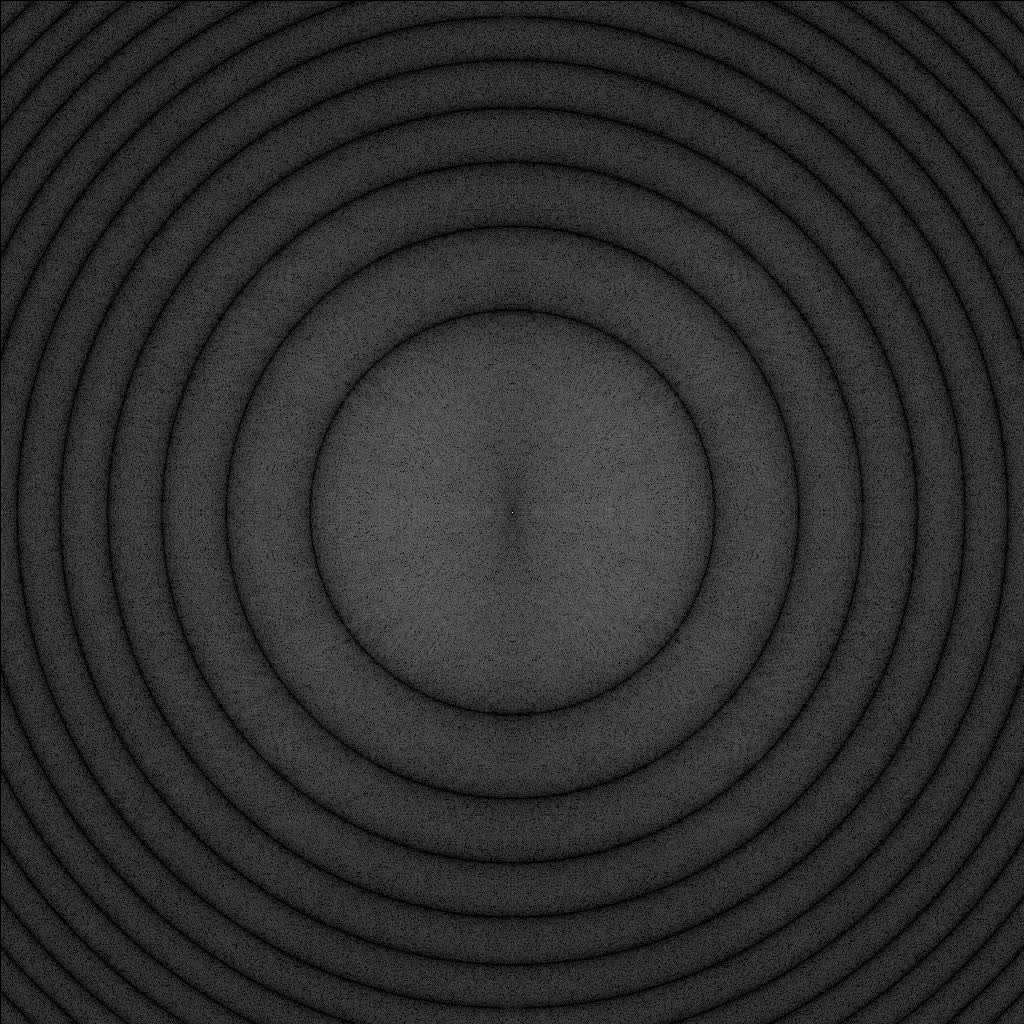
\includegraphics[height=\imh]
          {videos/intensity/FT-intensity_vs_distance.jpg}}
      };         
      \node[inner sep=1pt,below] at (0,0){$\abs{\F I_z}(\vecxi)$};
    \end{tikzpicture}
    %% RIGHT
    \column{0.6\textwidth}
  \begin{tikzpicture}
    \def\xx{0.55\textwidth};
    \def\imh{0.45\textwidth};
    \small
    % Image    
    \node[inner sep=0pt] at (0,0){
      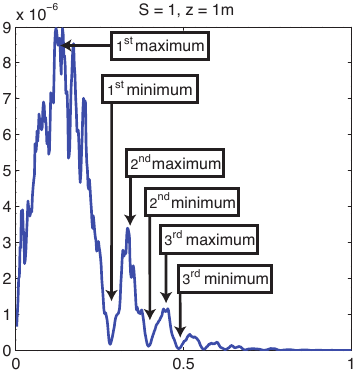
\includegraphics[height=\imh]{figures/minimum/angint-abs-ft-int}};         
    \node[inner sep=0pt,above,rotate=90] at (-\imh/2,0)
    {Line cut: $\abs{\F I_z}(\abs{\vecxi})$};
    \node[inner sep=1pt,below] at (0,-\imh/2){$\abs{\vecxi}/\xi_{\mathrm{c}}$};
    % Image    
    \node[inner sep=0pt] at (\xx,0){
      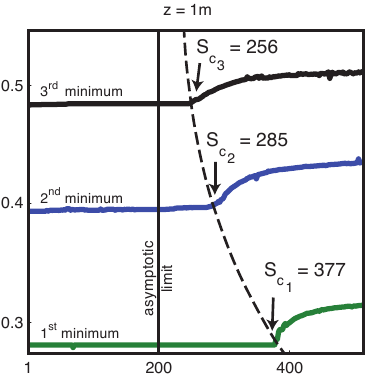
\includegraphics[height=\imh]{figures/minimum/minima-pos}};         
    \node[inner sep=0pt,above,rotate=90] at (\xx-\imh/2,0){min. pos. $\abs{\vecxi}_{\mathrm{min}}/\xi_{\mathrm{c}}$};
    \node[inner sep=1pt,below] at (\xx,-\imh/2){Upscaling $S$};
    \end{tikzpicture}
  \end{columns}
\end{frame}

%%%%%%%%%%%%%%%%%%%%%%%%%%%%%%%%%%%%%%%%%%%%%%%%%%%%%%%%%%%%%%%%%%%%%%
\begin{frame}
  \frametitle{Phase retrieval: quasiparticle approach}
  \begin{columns}[T]
    \column{0.35\textwidth}
    \begin{itemize}
    \item Fourier space filter: crop regions around minima
    \item Phase retrieval via CTF using filtered intensity
    \end{itemize}

    \begin{flushright}
      {\scriptsize Data: TopoTomo@ANKA}
    \end{flushright}
    \column{0.65\textwidth}
  \begin{tikzpicture}[]
    \def\xx{0.55\textwidth};
    \def\imh{0.37\textwidth};
    \def\yy{1.3*\imh}
    \small
    % intensity
    \node[inner sep=1pt,above] at (\xx,0){
      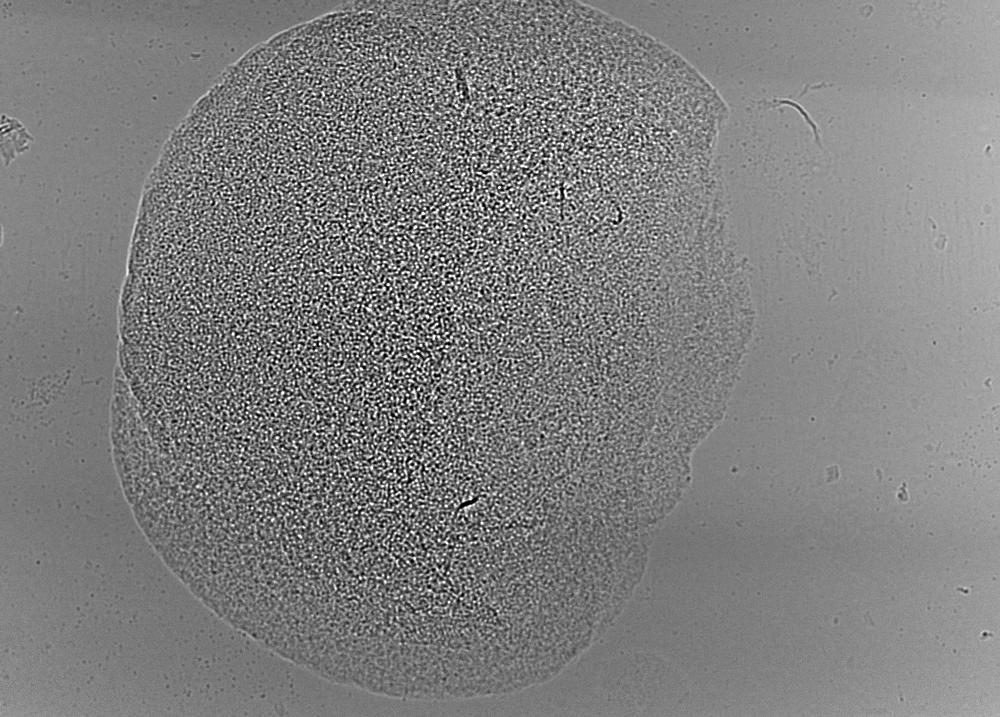
\includegraphics[height=\imh]{figures/ctf-filtering/CTFfiltering_intensity}};         
    \node[inner sep=1pt,below] at (\xx,0){$I_z$};
    % FT intensity
    \node[inner sep=1pt,above] at (2*\xx,0){
      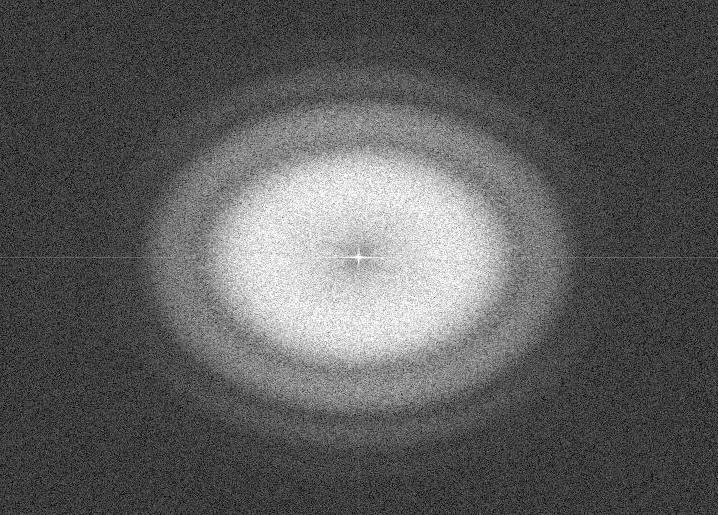
\includegraphics[height=\imh]{figures/ctf-filtering/CTFfiltering_intensityFTabs}};         
    \node[inner sep=1pt,below] at (2*\xx,0){$\abs{\F I_z}$};
    % binary filter
    \node[inner sep=1pt,above] at (\xx,-\yy){
      
\includegraphics[height=\imh]{figures/ctf-filtering/CTFfiltering_binaryfilter}};         
    \node[inner sep=1pt,below] at (\xx,-\yy){binary filter};
    % FT intensity
    \node[inner sep=1pt,above] at (2*\xx,-\yy){
      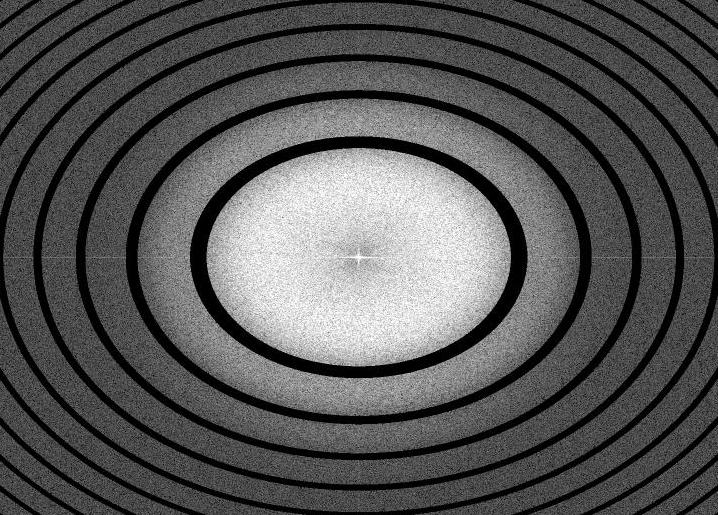
\includegraphics[height=\imh]{figures/ctf-filtering/CTFfiltering_intensityFTabsBinFilt}};         
    \node[inner sep=1pt,below] at (2*\xx,-\yy){filtered $\abs{\F I_z}$};
    \end{tikzpicture}
  \end{columns}

  \reff{Moosmann et al., Opt. Express 2011}
\end{frame}

%%%%%%%%%%%%%%%%%%%%%%%%%%%%%%%%%%%%%%%%%%%%%%%%%%%%%%%%%%%%%%%%%%%%%%
\begin{frame}
  \frametitle{Tomography: Paganin vs CTF vs QP} 

  Xenopus, fixed, 4-cell stage, ID19@ESRF, $E=\SI{20}{keV}$, $\Delta
    E/E=\num{e-4}$, $z=$\SI{1}{m}, $\Delta~x=\SI{0.75}{\micro\metre}$, 1600 projections
\begin{tikzpicture}[]
    \def\imh{0.28\textwidth}
    \small
    \node[inner sep=1pt,above] at (0,0){
      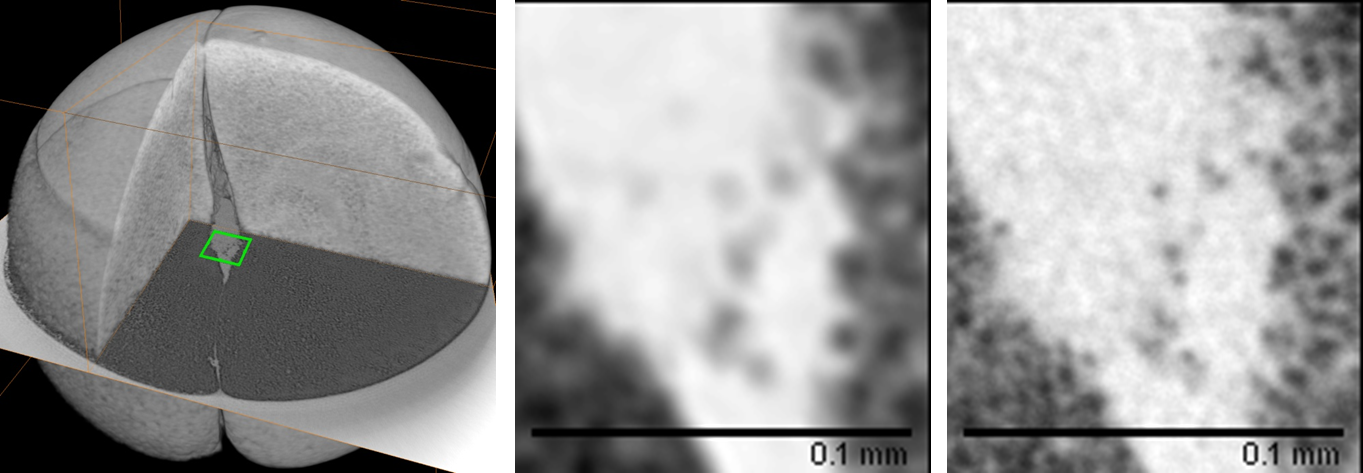
\includegraphics[height=\imh]{figures/paganin-ctf-qp/rend-pag-qp}};         
    \node[inner sep=1pt,below] at (-0.9*\imh,0){Rendering};
    \node[inner sep=1pt,below] at (0.1*\imh,0){Paganin};
    \node[inner sep=1pt,below] at (\imh,0){Quasiparticle};
    \end{tikzpicture}
  \begin{tikzpicture}[]
    \def\imh{0.3\textwidth}
    \small
    \node[inner sep=1pt,above] at (0,0){
      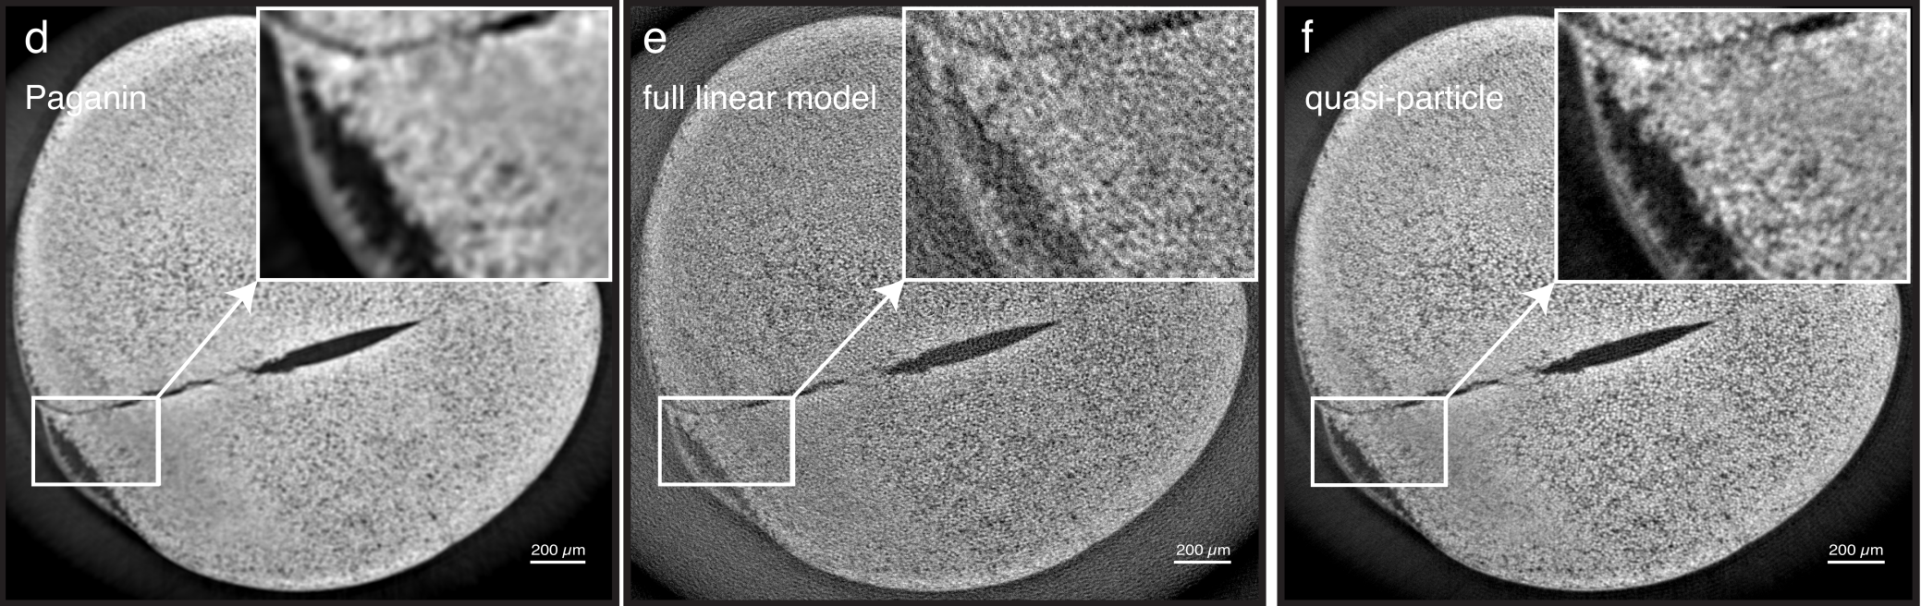
\includegraphics[height=\imh]{figures/paganin-ctf-qp/pag-ctf-qp}};         
    \node[inner sep=1pt,below] at (-\imh,0){Paganin};
    \node[inner sep=1pt,below] at (0,0){CTF};
    \node[inner sep=1pt,below] at (\imh,0){Quasiparticle};
    \end{tikzpicture}
\end{frame}

%%%%%%%%%%%%%%%%%%%%%%%%%%%%%%%%%%%%%%%%%%%%%%%%%%%%%%%%%%%%%%%%%%%%%%
\begin{frame}
  \frametitle{In vivo tomography: Paganin vs QP} 

  Xenopus, in vivo, stage 23, ID19@ESRF, $E=\SI{26.2}{keV}$, $\Delta
  E/E\approx\num{0.15}$ (single harmonic), $z=$\SI{3.6}{m},
  $\Delta~x=\SI{1.6}{\micro\metre}$, 500 projections

\begin{tikzpicture}[]
  \def\imh{0.33\textheight}
  \def\xx{0.33\textwidth}
  \small
  % left
  \node[above] at (0,0){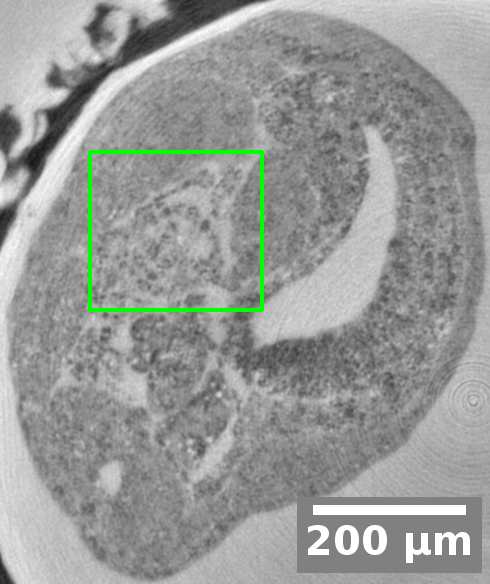
\includegraphics[height=\imh]
    {figures/qp-vs-tie-stage23/xeno-qp-full.png}};         
  \node[below] at (0,0){tomogram slice};
  % middle
  \node[above] at (\xx,0){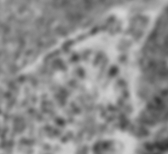
\includegraphics[height=\imh]
    {figures/qp-vs-tie-stage23/xeno-tie-roi.png}};
  \node[below] at (\xx,0){Paganin, zoom};
  % right
  \node[above] at (2*\xx,0){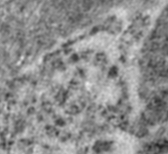
\includegraphics[height=\imh]
    {figures/qp-vs-tie-stage23/xeno-qp-roi.png}};
  \node[below] at (2*\xx,0){quasiparticle, zoom};
\end{tikzpicture}
\end{frame}

%%%%%%%%%%%%%%%%%%%%%%%%%%%%%%%%%%%%%%%%%%%%%%%%%%%%%%%%%%%%%%%%%%%%%%
%%%%%%%%%%%%%%%%%%%%%%%%%%%%%%%%%%%%%%%%%%%%%%%%%%%%%%%%%%%%%%%%%%%%%%
\section{In vivo X-ray phase-contrast tomography}

%%%%%%%%%%%%%%%%%%%%%%%%%%%%%%%%%%%%%%%%%%%%%%%%%%%%%%%%%%%%%%%%%%%%%%
%%%%%%%%%%%%%%%%%%%%%%%%%%%%%%%%%%%%%%%%%%%%%%%%%%%%%%%%%%%%%%%%%%%%%%
\subsection{Motivation}

%%%%%%%%%%%%%%%%%%%%%%%%%%%%%%%%%%%%%%%%%%%%%%%%%%%%%%%%%%%%%%%%%%%%%%
\begin{frame}
  \frametitle{Motivation: in vivo imaging}
  \begin{itemize}
  \item Applications in Life Sciences: Imaging techniques to study the
    development of model organisms are essential tools in
    Developmental Biology, Medicine, Toxicology, Zoology, …
  \item Aim: Visualisation of developmental processes
    \begin{itemize}
    \item Division, differentiation, shape changes, \& trajectories of
      single cells
    \item Identify (new) morphological structures
    \item Movement \& separation of tissues
    \item Cavity formation
    \item Propulsion mechanism
    \end{itemize}

  \item Biological specimen w/o cartilage, bone, \& blood vessels are
    essentially pure-phase objects for $E>\SI{20}{keV}$
  \item Examples of important vertebrate model organisms
      \begin{tikzpicture}[]
        \def\xx{0.33\textwidth}
        \def\imh{0.22\textheight}
        \small
         \node[inner sep=1pt,above] at (-\xx,0){
           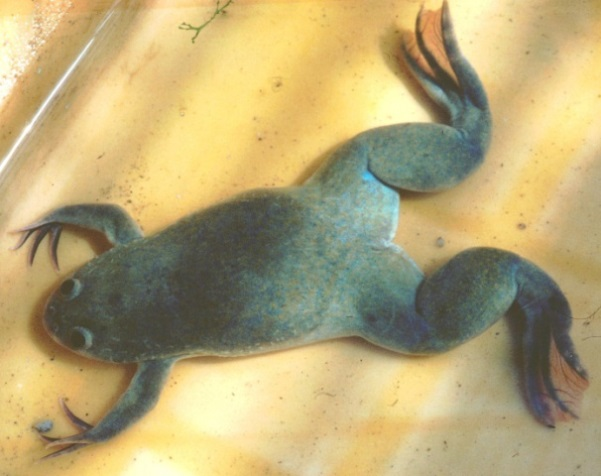
\includegraphics[height=\imh]{figures/model-organisms/xenopus}};         
         \node[inner sep=1pt,below] at (-\xx,0){Xenopus laevis};
         \node[inner sep=1pt,above] at (0,0){
           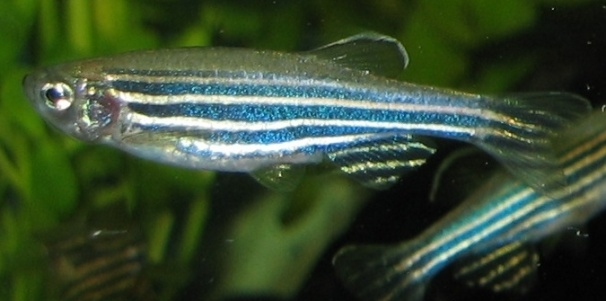
\includegraphics[height=\imh]{figures/model-organisms/zebrafish}};
         \node[inner sep=1pt,below] at (0,0){zebrafish};
         \node[inner sep=1pt,above] at (\xx,0){
           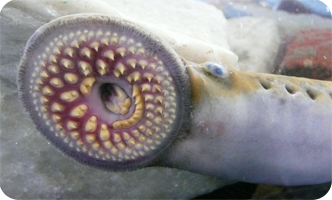
\includegraphics[height=\imh]{figures/model-organisms/lamprey}};
         \node[inner sep=1pt,below] at (\xx,0){lamprey};
    \end{tikzpicture}
  \end{itemize}
\end{frame}

%%%%%%%%%%%%%%%%%%%%%%%%%%%%%%%%%%%%%%%%%%%%%%%%%%%%%%%%%%%%%%%%%%%%%%
\subsection{Comparison with other techniques}

%%%%%%%%%%%%%%%%%%%%%%%%%%%%%%%%%%%%%%%%%%%%%%%%%%%%%%%%%%%%%%%%%%%%%%
\begin{frame}
  \frametitle{Comparison of in vivo imaging techniques}
  Optical light microscopy
    \begin{itemize}
      \item non-destructive
      \item restricted to surfaces or transparent samples
      \item destructive: sectioning of fixed embryos
      \item spatial resolution $\sim\SI{1}{\micro\metre}$
    \end{itemize}
    \begin{tikzpicture}
    \def\imh{0.3\textheight}
    \def\imw{0.3\textwidth}
    \def\xx{1.1*\imw}
    \small
%    \node[rotate=90] at (-1.5*\xx,0.5*\imh){Xenopus}; 
    % left
    \node[above] at (-\xx,0){
      \href{run:videos/comparison-optical/SingleCellToBlastula.mpg?autostart&loop}{
      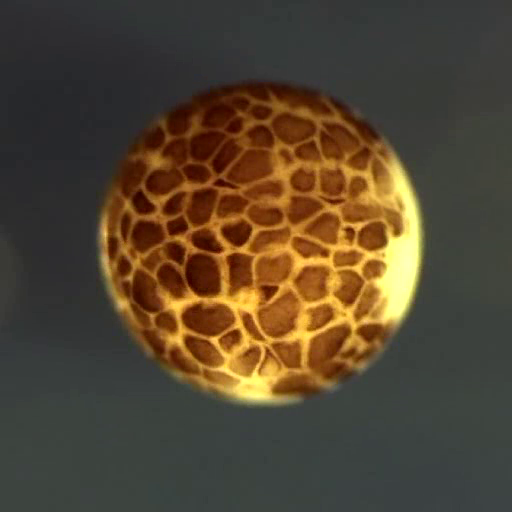
\includegraphics[height=\imh]{videos/comparison-optical/SingleCellToBlastula.png}}
    };         
    \node[below,align=center] at (-\xx,0){Xenopus: surface};
    % middle
    % \node[above] at (0,0){
    %   \href{run:videos/comparison-optical/GastrulationThroughNeurulationAndTailbud.mpg?autostart&loop}{
    %   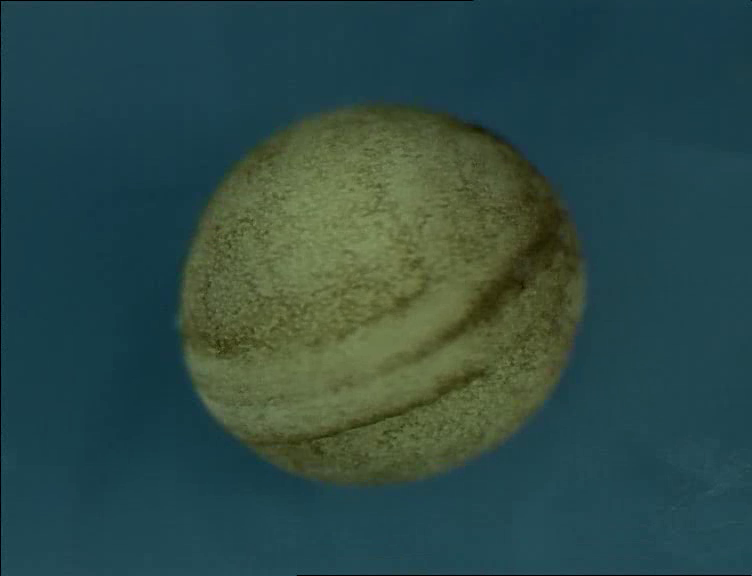
\includegraphics[height=\imh]{videos/comparison-optical/GastrulationThroughNeurulationAndTailbud.png}}
    % };         
    % \node[below,align=left] at (0,0){surface};
    \node[above] at (0,0){
      \href{run:videos/comparison-optical/xeno-optical-sectioning.avi?autostart&loop}{
      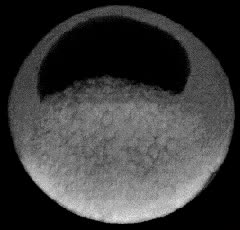
\includegraphics[height=\imh]{videos/comparison-optical/xeno-optical-sectioning.jpg}}
    };         
   \node[below,align=center] at (0,0){Xenopus: surface,\\ sectioned};
    right
    \node[above] at (\xx,0){
      \href{run:videos/comparison-optical/zebra-opt.mov?autostart&loop}{
      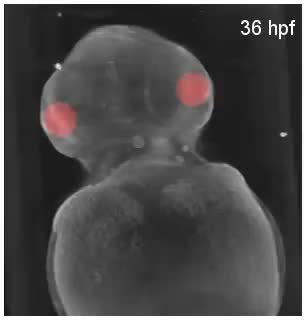
\includegraphics[height=\imh]{videos/comparison-optical/zebra-opt.jpg}}
    };         
   \node[below,align=center] at (\xx,0){Zebrafish: optical \\projection tomography};
    \end{tikzpicture}
    \reff{Williams \& Smith; Danilchik; Bassi et al.}
\end{frame}

%%%%%%%%%%%%%%%%%%%%%%%%%%%%%%%%%%%%%%%%%%%%%%%%%%%%%%%%%%%%%%%%%%%%%%
\begin{frame}
  \frametitle{Comparison of in vivo imaging techniques}
  Fluorescence microscopy 
  \begin{itemize}
  \item non-destructive
  \item transparent objects
  \item depth information limited to few cell layers
  \item Labelling: expression of fluorescence marker required
  \item photobleaching
  \item sparse spatial information 
  \item spatial resolution $\sim\SI{1}{\micro\metre}$
  \end{itemize}
  \begin{tikzpicture}
    \def\xx{0.225\textwidth}
    \def\imh{0.25\textheight}
    \small
    \node[above,rotate=90] at (-1.6*\xx,0.5*\imh) {Zebrafish};
    % light-sheet
    \node[above] at (-\xx,0){
      \href{run:videos/comparison-fluo/zebra-light-sheet.avi?autostart&loop}{
        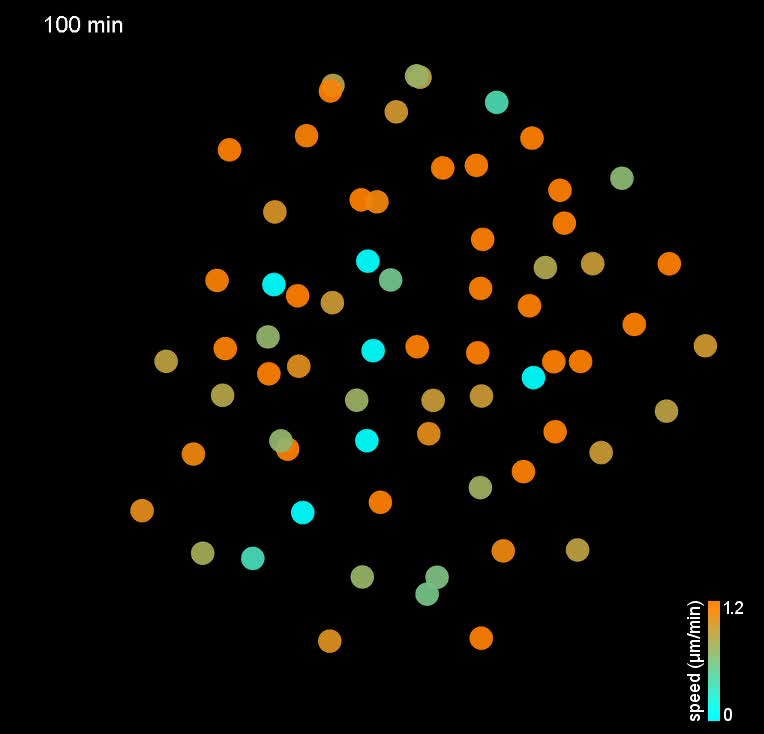
\includegraphics[height=\imh]{videos/comparison-fluo/zebra-light-sheet.jpg}}
    };
    \node[below,align=center] at (-\xx,0) {light-sheet microscopy};
    % \node[above] at (\xx,0){
    %   \href{run:videos/comparison-fluo/zebra-light-sheet_2.avi?autostart&loop}{
    %     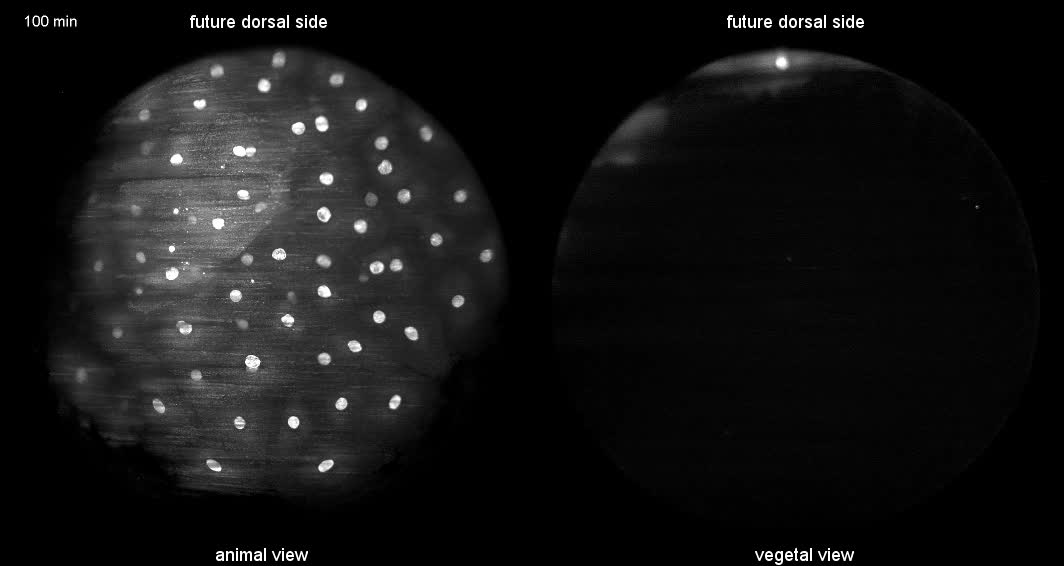
\includegraphics[height=\imh]{videos/comparison-fluo/zebra-light-sheet_2.jpg}}
    % };         
    % \node[below] at (0,0) {Zebrafish: light-sheet microscopy};
    % SPIM
    \node[above] at (\xx,0){
      \href{run:videos/comparison-fluo/zebra-spim.mov?autostart&loop}{
        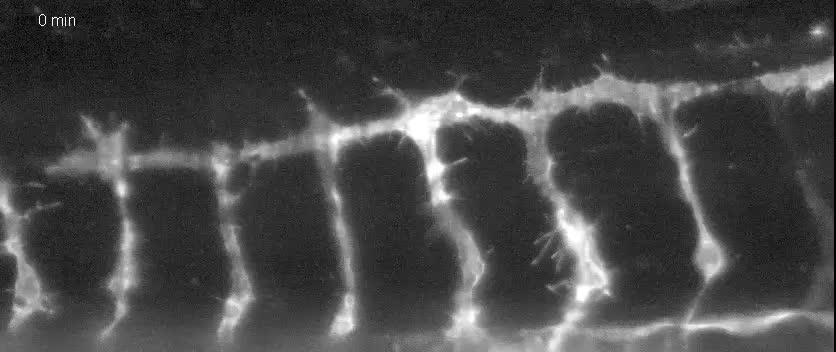
\includegraphics[height=\imh]{videos/comparison-fluo/zebra-spim.jpg}}
    };
    \node[below,align=center] at (\xx,0) {selective plane illumination microscopy};
  \end{tikzpicture}
\reff{Huisken et al.; Keller et al.}
\end{frame}

%%%%%%%%%%%%%%%%%%%%%%%%%%%%%%%%%%%%%%%%%%%%%%%%%%%%%%%%%%%%%%%%%%%%%%
\begin{frame} 
  \frametitle{Comparison of in vivo imaging techniques}
  Magnetic Resonance Imaging
  \begin{columns}[T]
    \column{0.5\textwidth}
  \begin{itemize}
  \item non-destructive 
  \item dense \& deep spatial information
  \item spatial resolution $\sim\SI{25}{\micro\metre}$
  \item temporal resolution $\sim\SI{1}{h/tomogram}$
  \end{itemize}
    \column{0.5\textwidth}
  \begin{tikzpicture}
    \def\imh{0.35\textheight}
    \small
    \node[above] at (0,0){
      \href{run:videos/comparison-mri/xeno-mri.avi?autostart&loop}{
        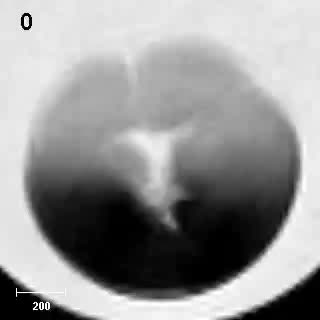
\includegraphics[height=\imh]{videos/comparison-mri/xeno-mri.jpg}}
    };         
    \node[below] at (0,0){Xenopus: MRI};
    \end{tikzpicture}
\reff{Papan et al.}
  \end{columns}
\end{frame}

%%%%%%%%%%%%%%%%%%%%%%%%%%%%%%%%%%%%%%%%%%%%%%%%%%%%%%%%%%%%%%%%%%%%%%
\begin{frame}
  \frametitle{Comparison of in vivo imaging techniques}
  X-ray phase-contrast microtomography (PC$\mu$CT)
  \begin{itemize}
  \item apt for optically opaque objects
  \item fast
  \item dense spatial information
  \item destructive: possible time lapse $\lesssim$ \SI{2}{h}
  \item spatial resolution $\sim\SI{1}{\micro\metre}$
  \end{itemize}    
  \begin{tikzpicture}
    \node[above] at (0,0){
      \href{run:videos/comparison-xray/nature-movie_03.avi?autostart&loop}{
        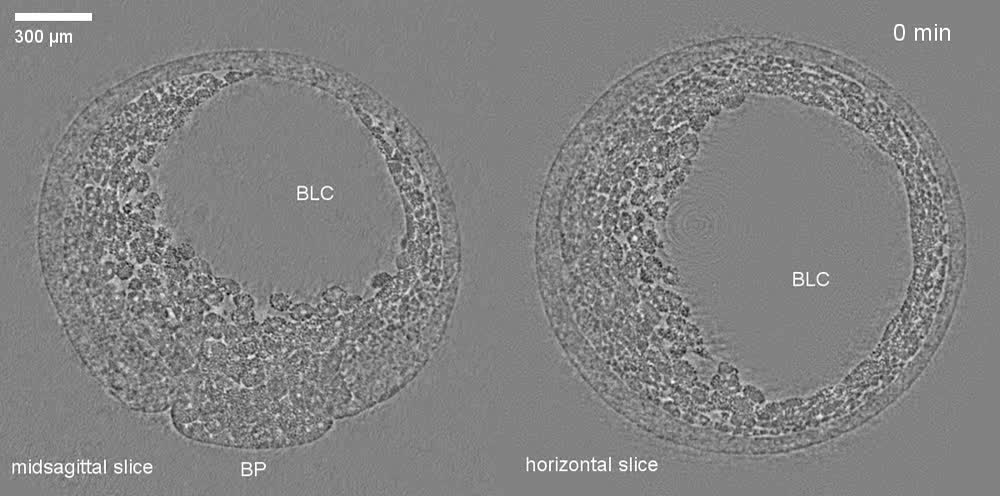
\includegraphics[height=0.3\textheight
        ]{videos/comparison-xray/nature-movie_03.jpg}}};
    \node[below] at (0,0){Xenopus: X-ray PC$\mu$CT};
\end{tikzpicture}
    % {\footnotesize 
    %   2-BM@APS\\ 
    %   energy $E=\SI{30}{keV}$,
    %   object-detector dist. $z$=\SI{62}{cm}\\
    %   pixel size $\Delta x$=\SI{1}{\micro\metre}\\
    %   bandwidth $\Delta E/E$=\num{e-2}\\
    %   exposure time/image $\Delta t$=\SI{15}{ms}\\
    %   time lapse $\sim\SI{2}{h}$
    % }
  \reff{Moosmann et al., Nature;
    Moosmann et al., Nature Protocols
  %  ;Nawy, Nature Methods (research highlight)
  }
\end{frame}

%%%%%%%%%%%%%%%%%%%%%%%%%%%%%%%%%%%%%%%%%%%%%%%%%%%%%%%%%%%%%%%%%%%%%%
\begin{frame}
  \frametitle{Digital study}
  Using dense \& deep 3D information allows to digitally study
  \begin{itemize}
  \item Structural changes, gene expression, perturbation experiments 
    (signal transduction, functioning of gene regulatory networks, ...)
  \item Cell and tissue dynamics: exchange of fluids and nutrients,
    transient structures, cell migratory behaviour, ...
  \item Propulsion mechanisms for cell and tissue migration:
    differential flow-field analysis (convergent extension, cell-cell
    adhesion, cell-matrix interaction, ...)
  \end{itemize}
\end{frame}

%%%%%%%%%%%%%%%%%%%%%%%%%%%%%%%%%%%%%%%%%%%%%%%%%%%%%%%%%%%%%%%%%%%%%%
\subsection{Considerations for in vivo imaging}

%%%%%%%%%%%%%%%%%%%%%%%%%%%%%%%%%%%%%%%%%%%%%%%%%%%%%%%%%%%%%%%%%%%%%%
\begin{frame}
  \frametitle{Considerations for in vivo imaging}
  \begin{itemize}
  \item Motion blurring due to cell movement: $\sim \SI{4}{\micro\metre/min}$
    \begin{itemize}
    \item Acquisition time for tomogram at  resolution: $\lesssim \SI{30}{s}$
    \item Required flux density: $> \SI{e12}{photons/s/mm^2}$
    \end{itemize}

  \item Dose effects: heat load, double-strand breaking, radiolysis of
    water $\rightarrow$ free radicals
  \item Setup: parameter optimisation
    \begin{itemize}
    \item Energy: dose vs photon flux vs phase contrast vs detection efficiency
    \item Exposure time: dose vs signal-to-noise vs motion blurring
    \item Object-detector distance: signal-to-noise vs blurring
      (finite source size, coherence, nonlinear propagation effects)
    \item Tomography: number of projection, dose, resolution, rotation
      blurring, ...
    \end{itemize}
  \end{itemize}
\end{frame}

%%%%%%%%%%%%%%%%%%%%%%%%%%%%%%%%%%%%%%%%%%%%%%%%%%%%%%%%%%%%%%%%%%%%%%
\begin{frame}
  \frametitle{Dose effect: heat load}
  Compare simulation and measurement of temperature profile
  \begin{itemize}
  \item Simulation of temperature profile: solve heat equation numerically, energy:
    $\SI{30}{keV}$, flux: $\SI{e12}{photons/s/mm/square}$
  \end{itemize}

  \begin{tikzpicture}[]
    \def\xx{0.33\textwidth}
    \def\imh{0.33\textheight}
    \small
    \node[inner sep=1pt,above] at (-\xx,0){
      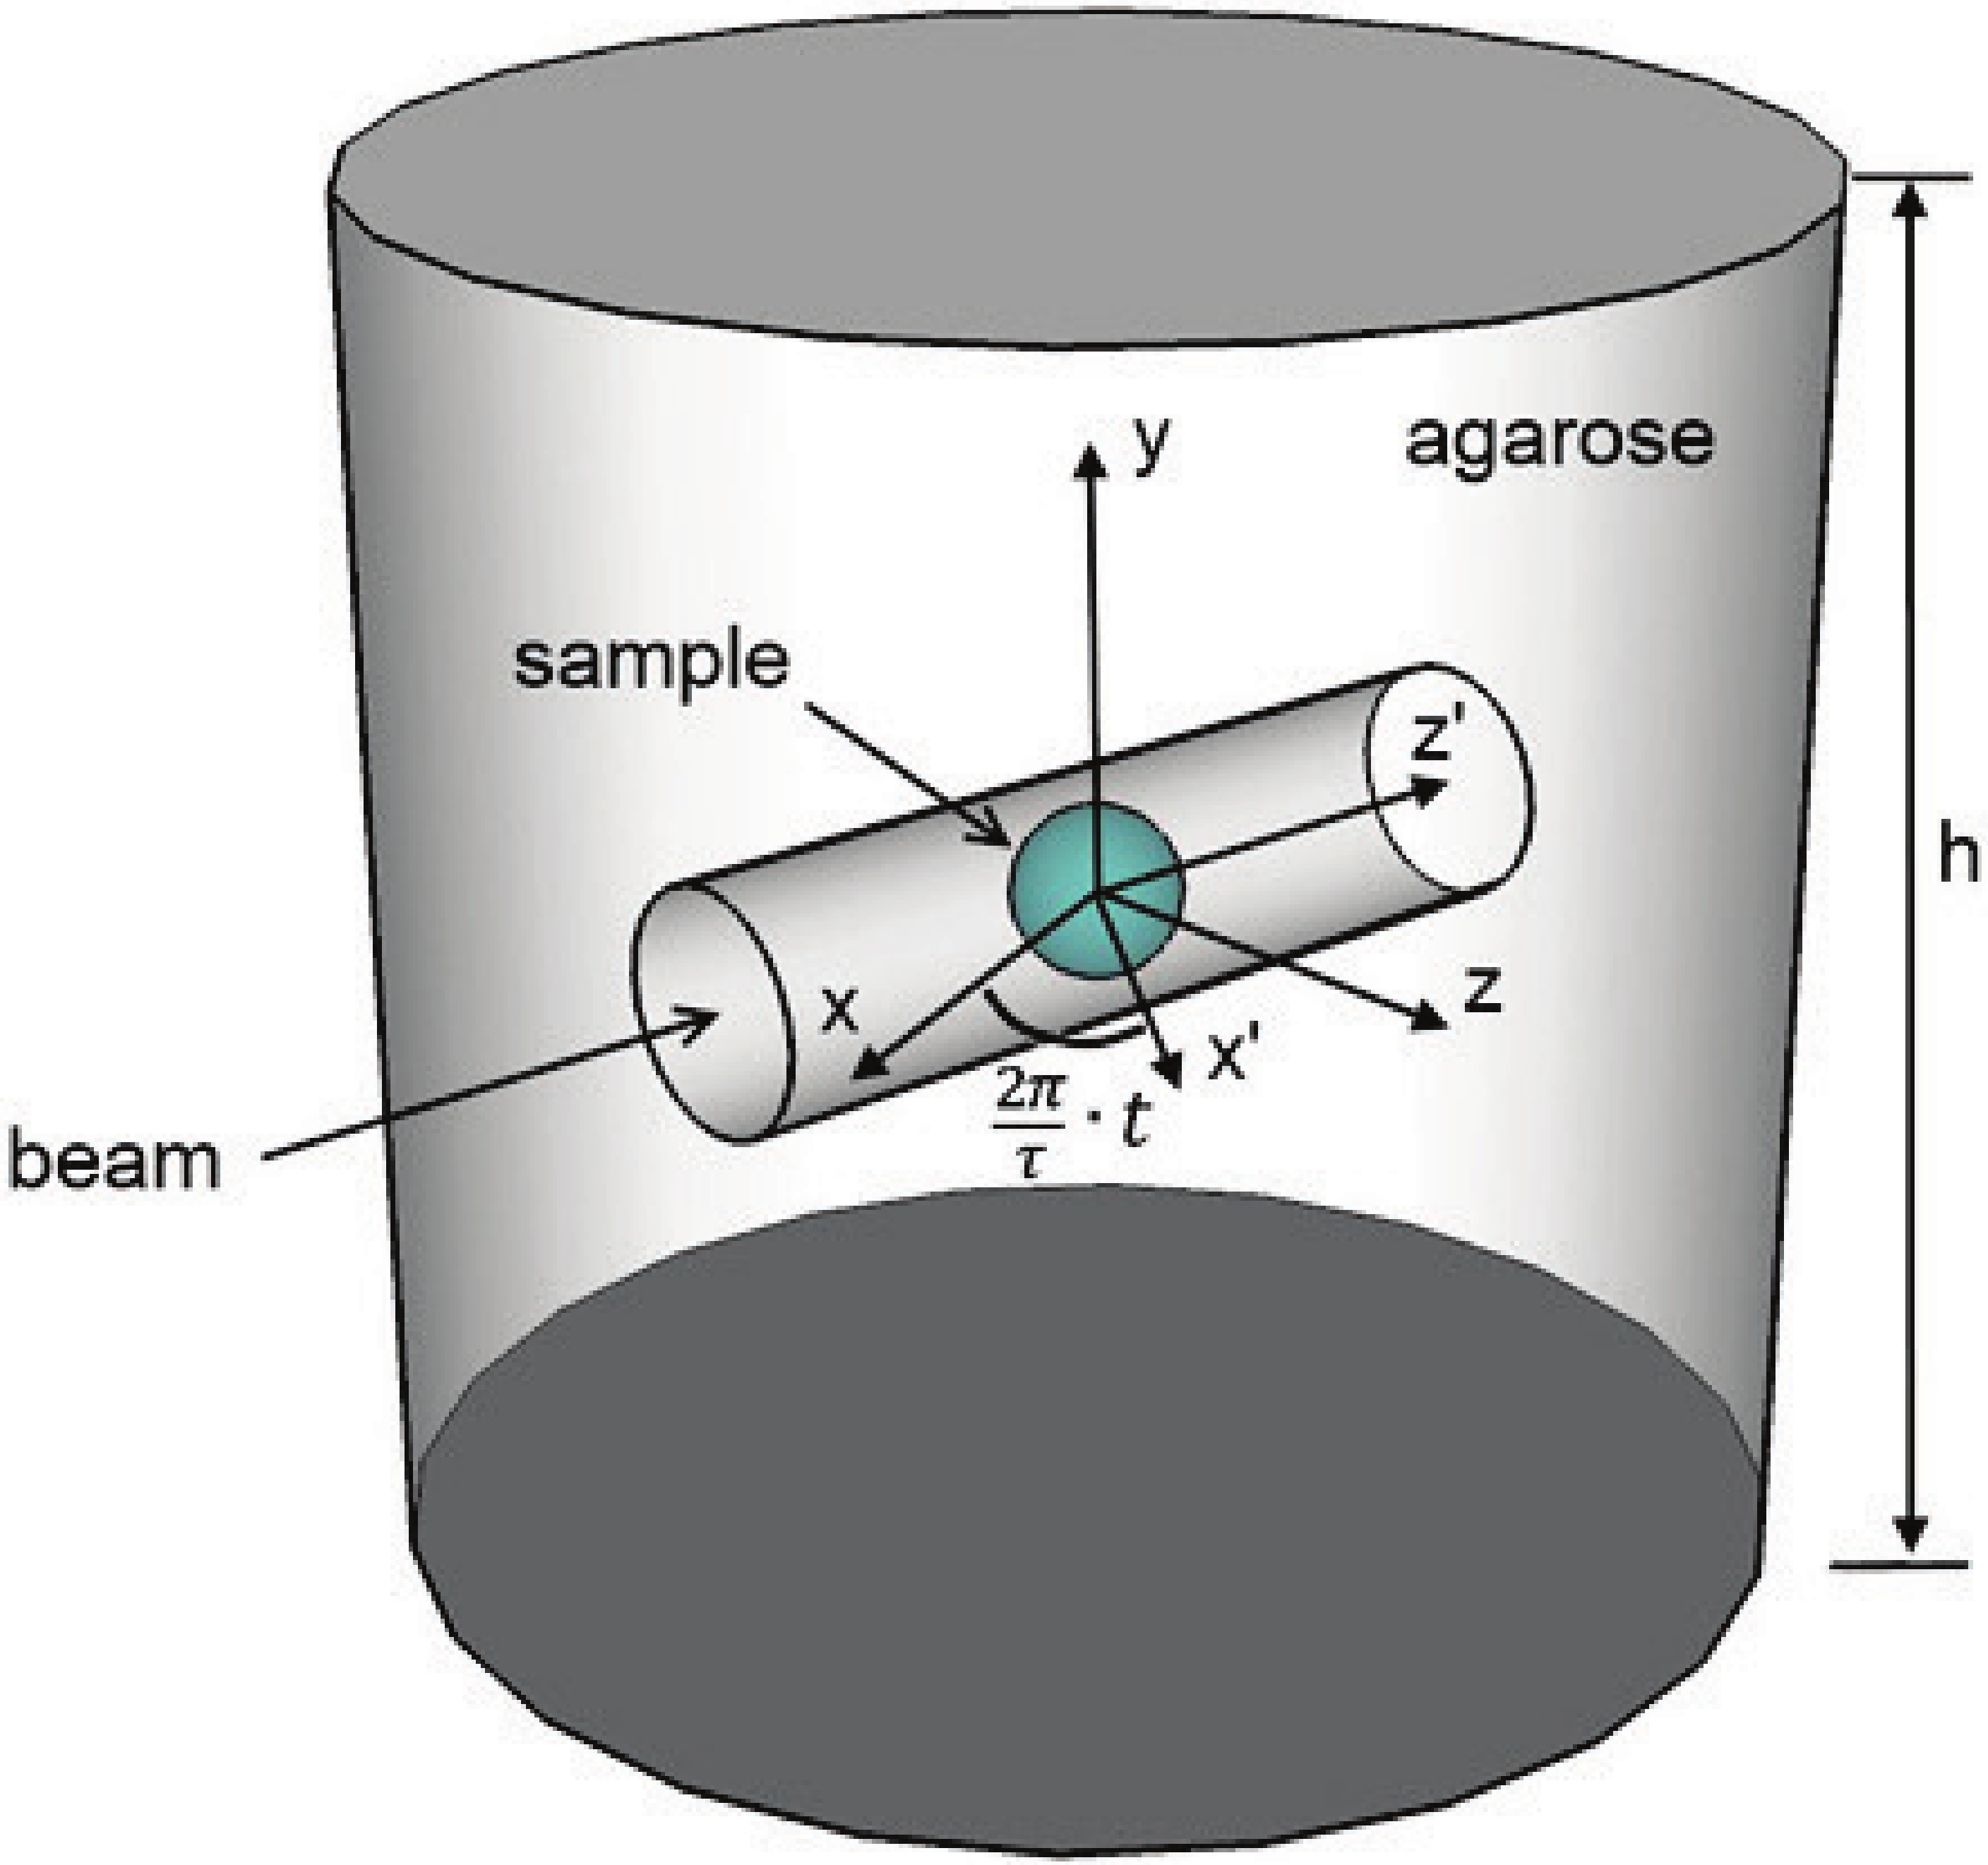
\includegraphics[height=\imh]{figures/heat-load/SampleAndBeam.png}};
    \node[inner sep=1pt,below, align=center] at (-\xx,0){schematic of\\ sample environment};
%    \node[right,align=left] at (0,2*\yy){Xenopus:\\ optical,\\ sectioned};
    \node[inner sep=1pt,above] at (0,0){
      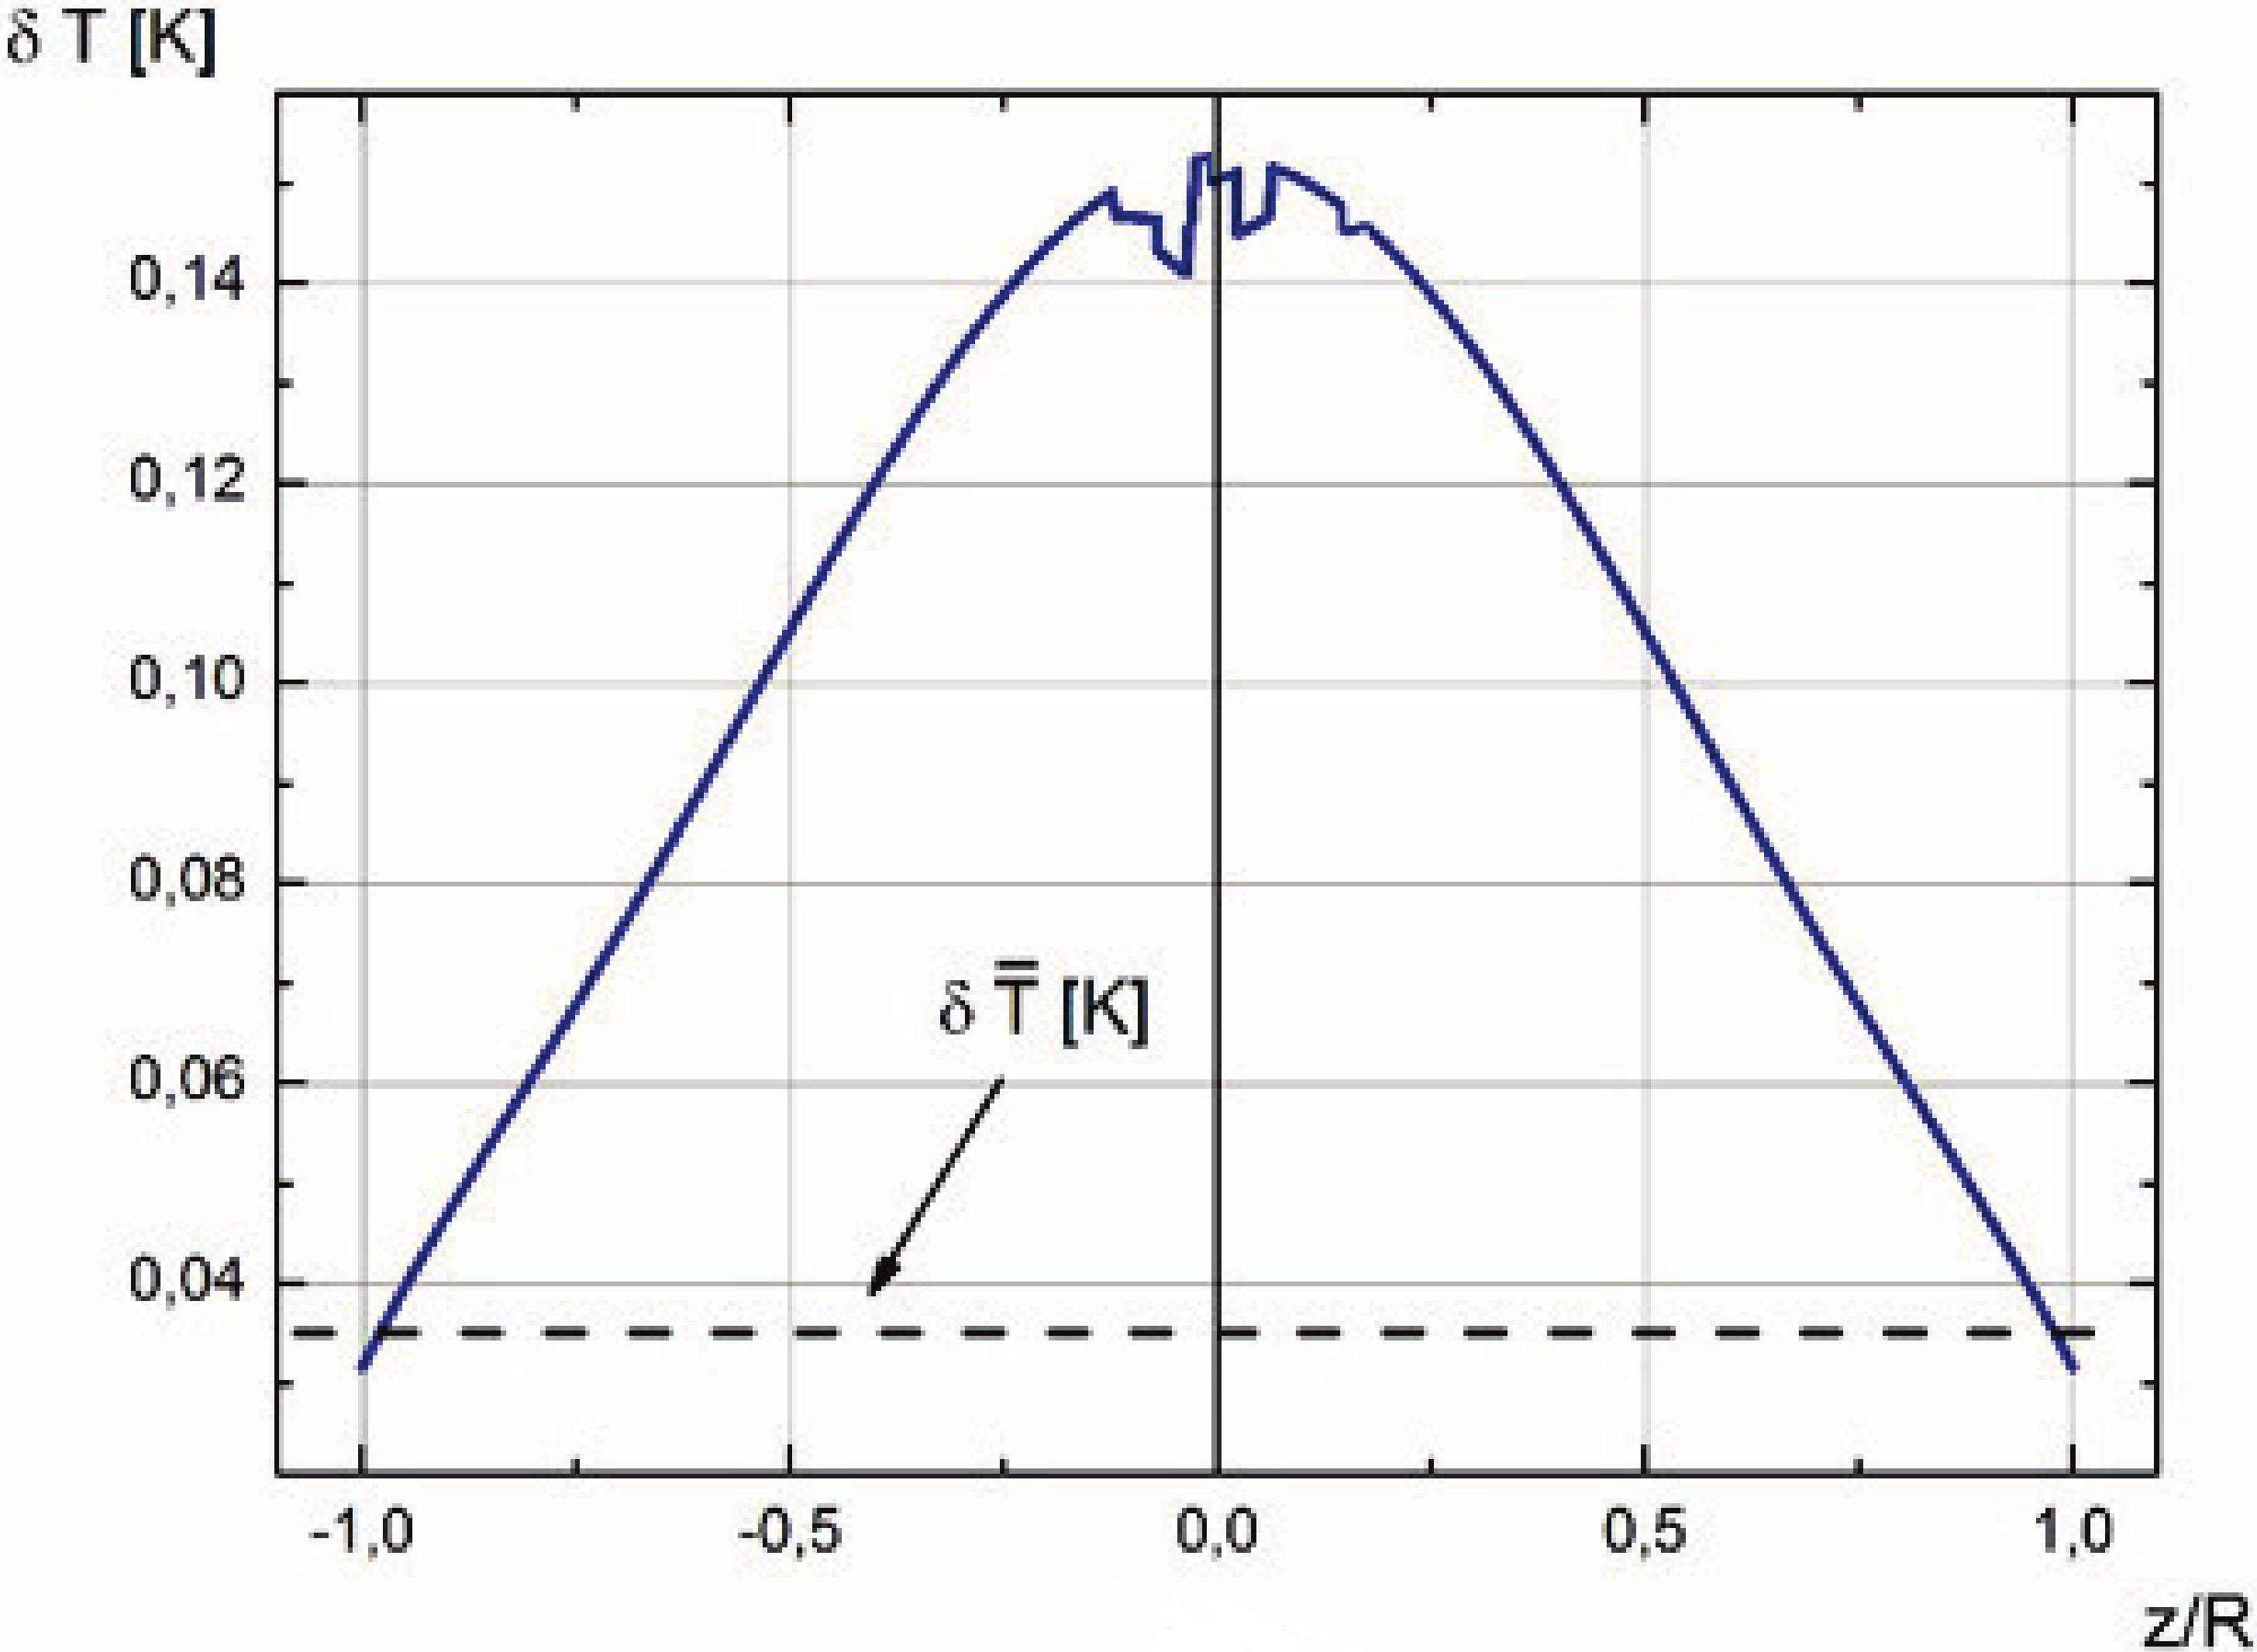
\includegraphics[height=\imh]{figures/heat-load/RadialTempProfile.png}};
    \node[inner sep=1pt,below,align=center] at (0,0){radial \\temperature profile};
    \node[inner sep=1pt,above] at (\xx,0){
      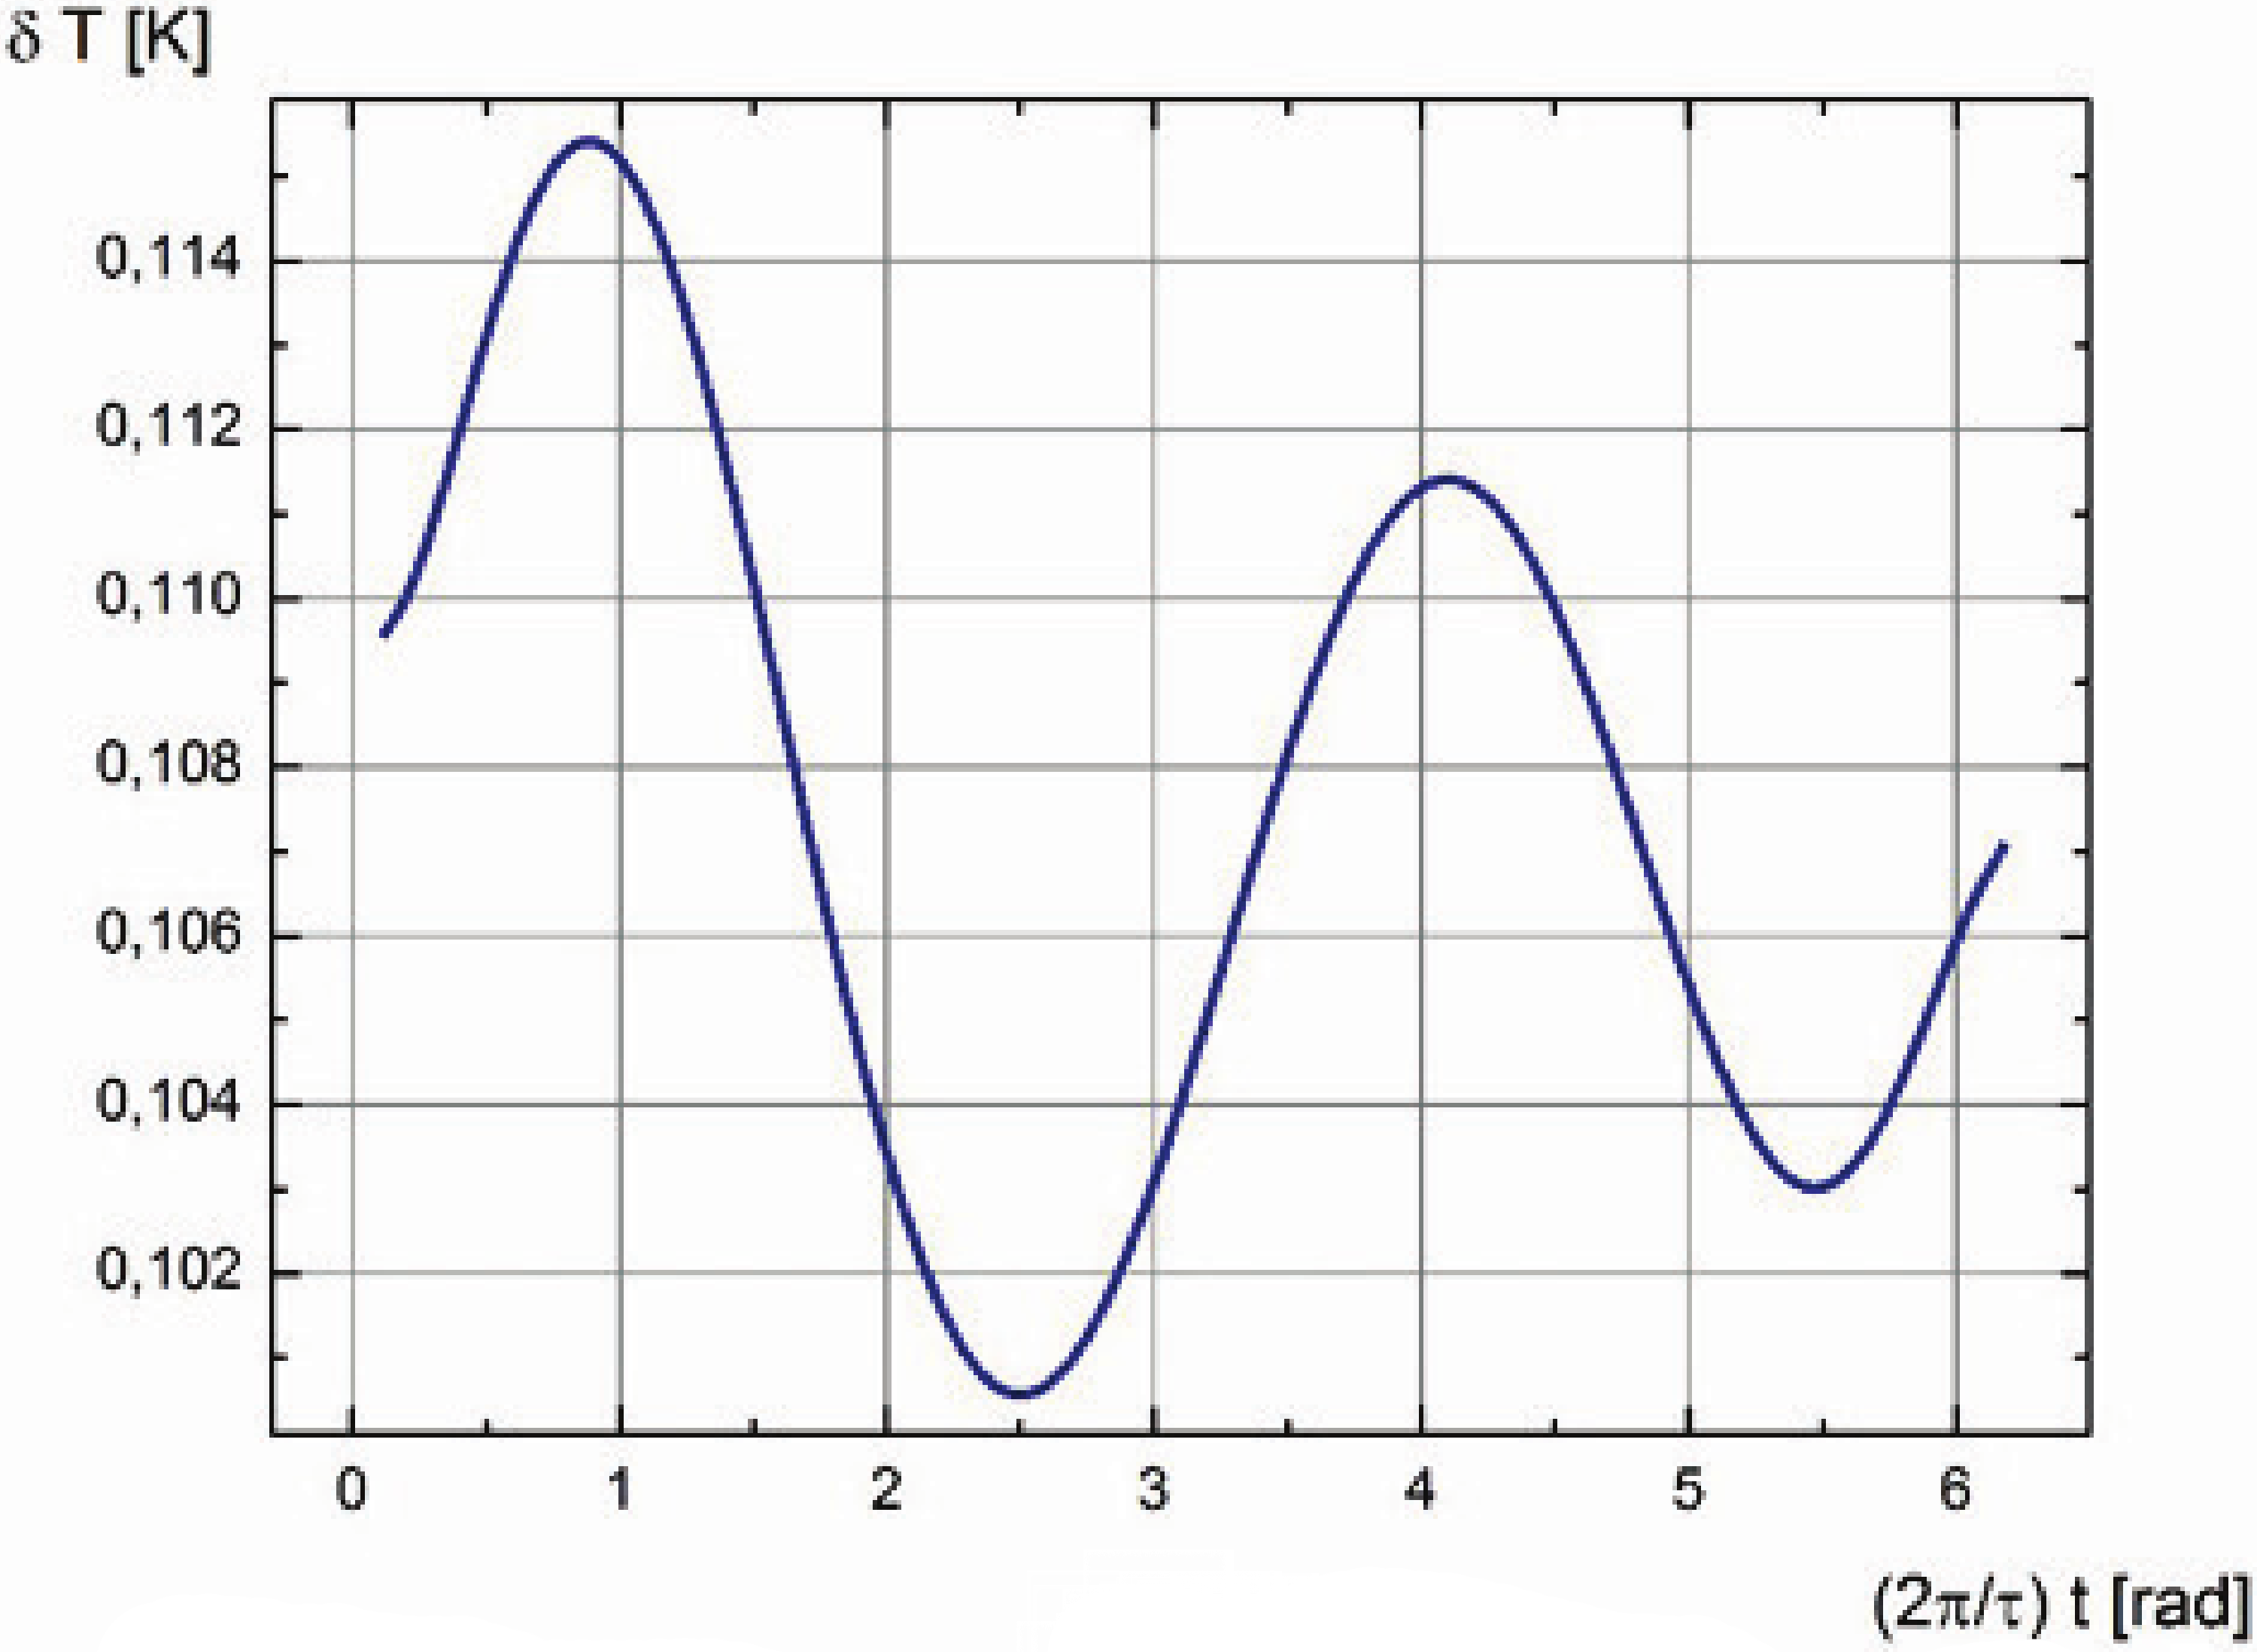
\includegraphics[height=\imh]{figures/heat-load/AngularTempProfile.png}};
    \node[inner sep=1pt,below,align=center] at (\xx,0){angular \\temperature profile};
  \end{tikzpicture}
\end{frame}

%%%%%%%%%%%%%%%%%%%%%%%%%%%%%%%%%%%%%%%%%%%%%%%%%%%%%%%%%%%%%%%%%%%%%%
\begin{frame}
  \frametitle{Dose effect: heat load}
  \begin{itemize}
  \item Measurement of temperature: setup identical to in vivo experiment
  \end{itemize}
  \begin{tikzpicture}[]
    \def\imw{0.85\textwidth}
    \def\xx{0.9\textwidth}
    \def\yy{0.2\textheight}
    \small
    \node[] at (0,0){
      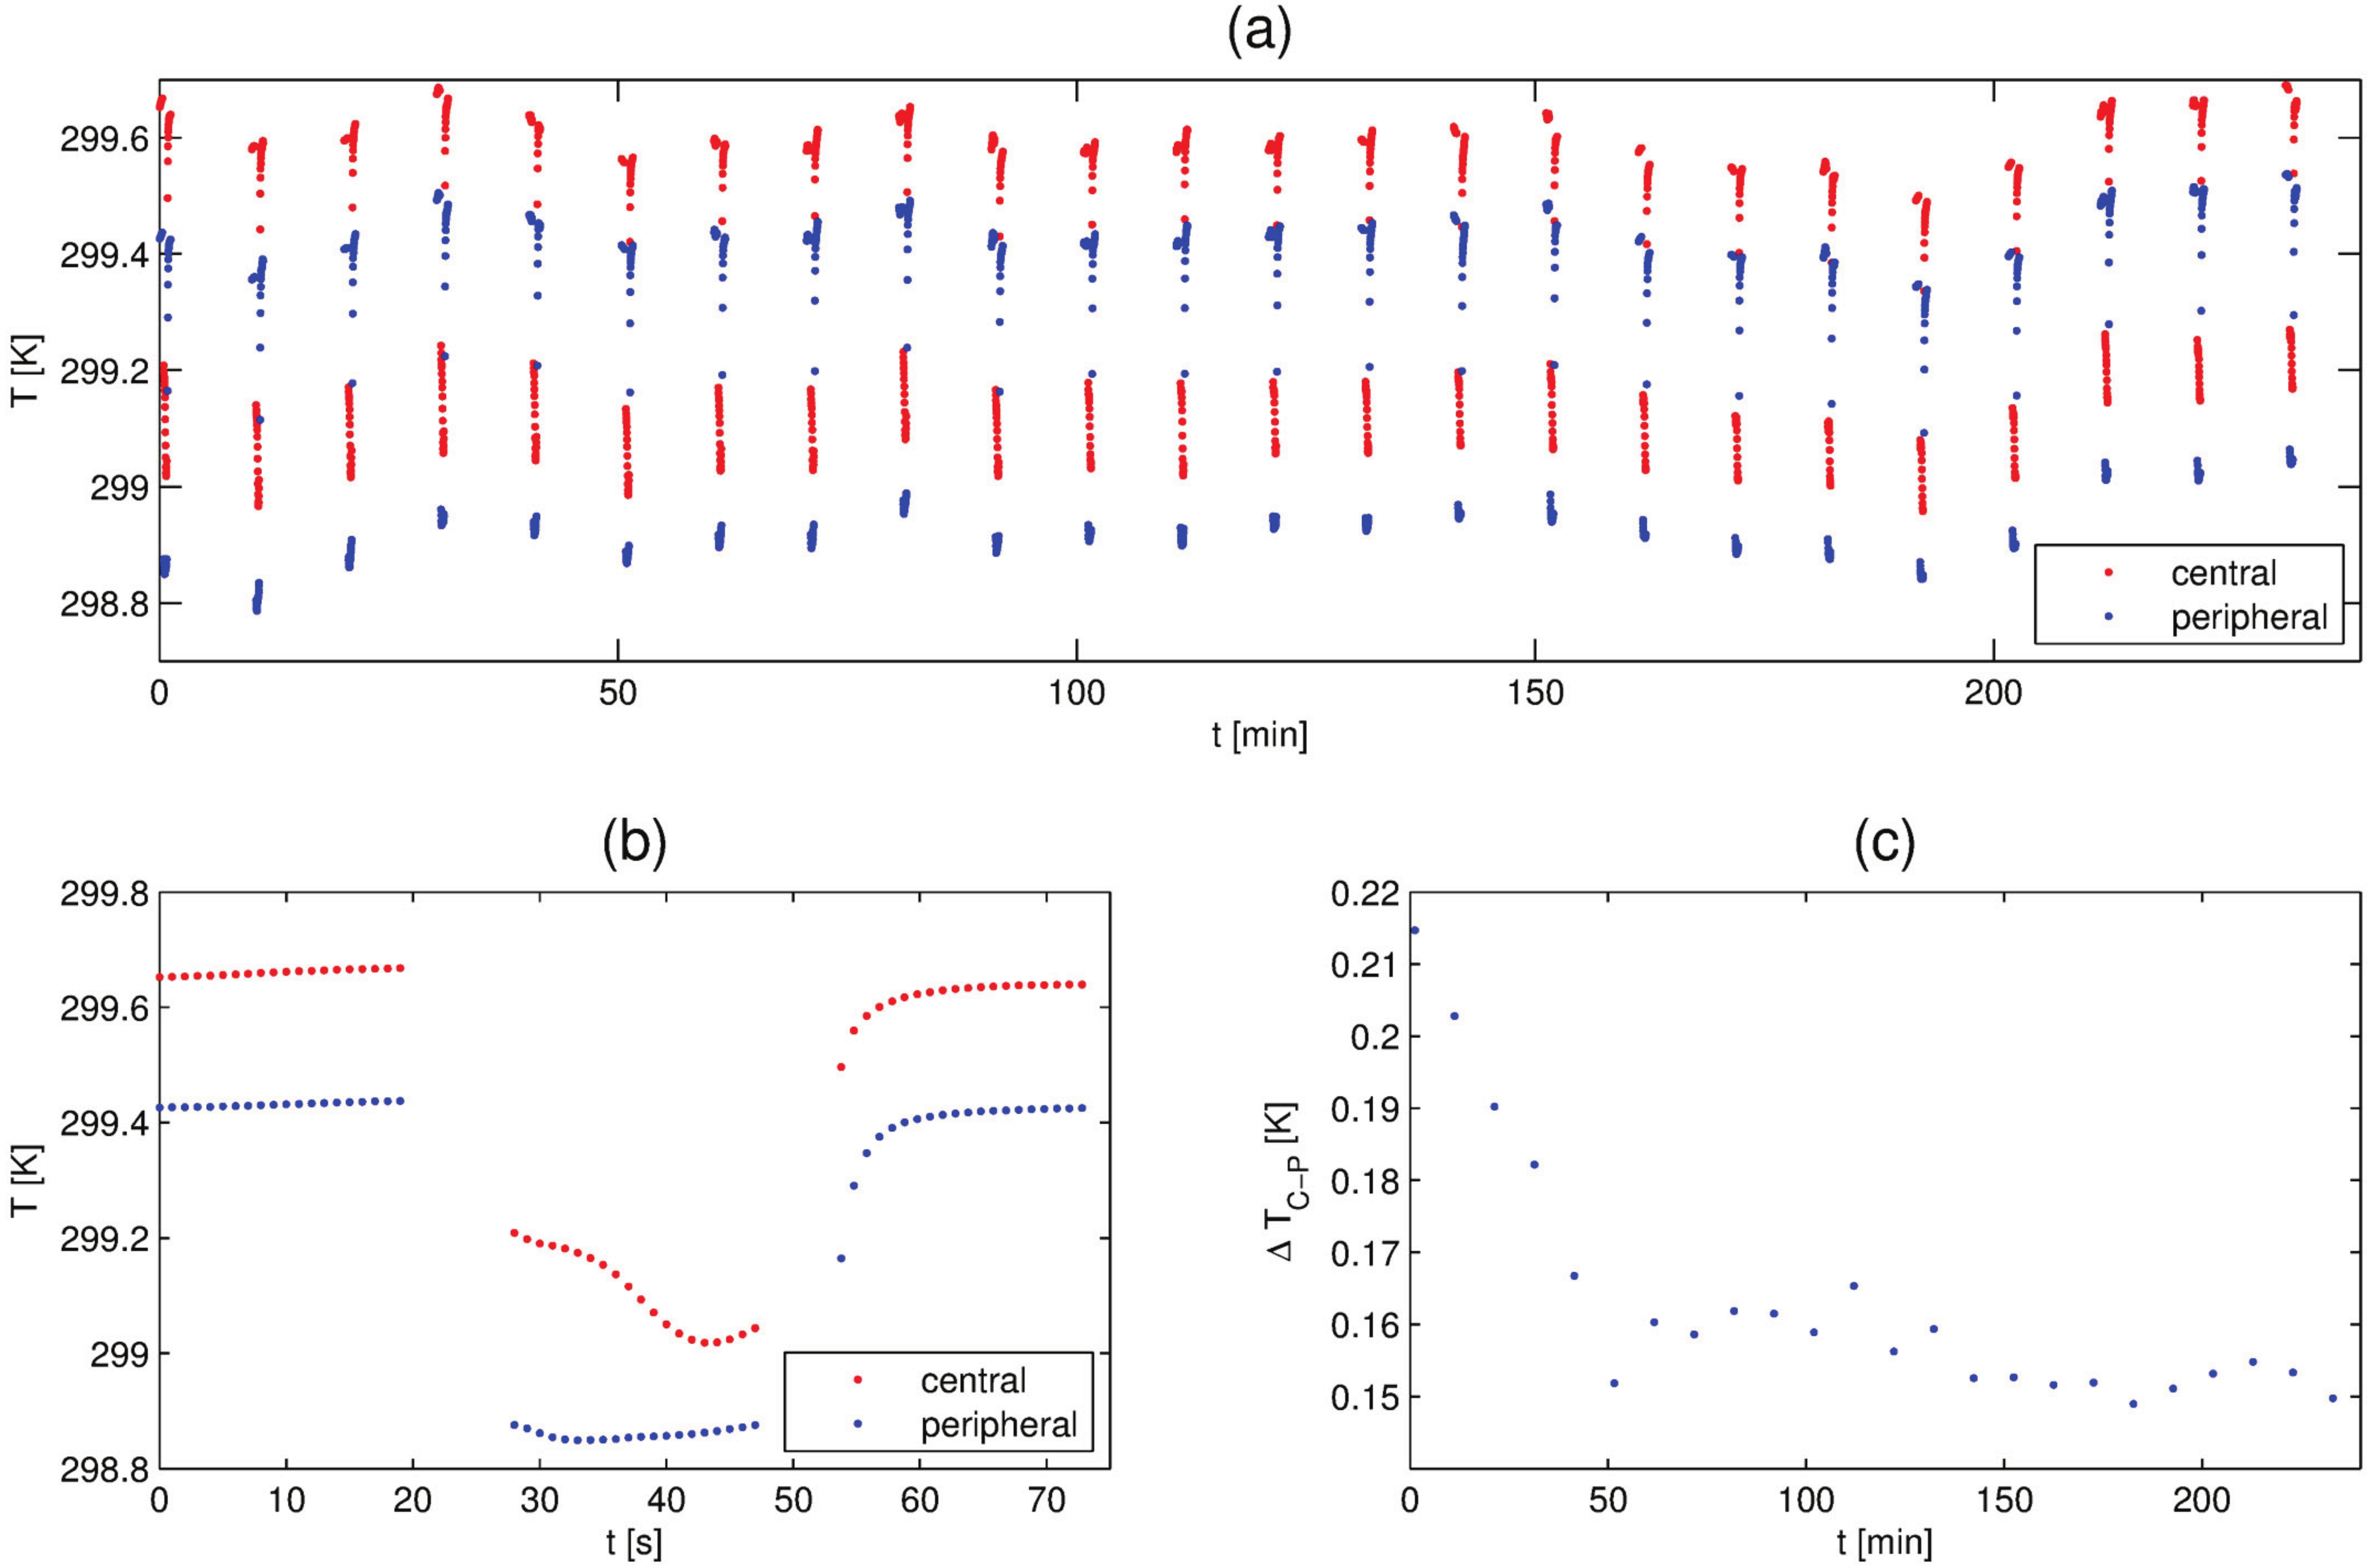
\includegraphics[width=\imw]{figures/heat-load/ExpTempProfile.png}};
    \node[rotate=90] at (-\xx/2,\yy){24 cycles};
    \node[rotate=90] at (-\xx/2,-\yy){1 cycle};
    \node[rotate=90] at (0,-\yy){24 cycles};
    \node[fill=white!100,above] at (-0.9*\xx/4,-0.45){before\quad\; during\quad\; after};
    \node[below] at (-0.9*\xx/4,-0.4){exposure};
    \node[fill=white!100] at (1.15*\xx/4,-0.2){central - peripheral Temp.};
    \node[] at (1.3*\xx/4,-0.8)
    {${\Delta T_{C-P}=\color{red}T_C}- {\color{blue}T_P}$ };
  \end{tikzpicture}
\end{frame}

%%%%%%%%%%%%%%%%%%%%%%%%%%%%%%%%%%%%%%%%%%%%%%%%%%%%%%%%%%%%%%%%%%%%%%
\begin{frame}
  \frametitle{Dose effect: radiolysis of water}
  Ionising radiation induces radiolysis of water molecules
  \begin{itemize}
  \item Radicals ($\scriptstyle H_3O^+$, $\scriptstyle HO\cdot$,
    $\scriptstyle e^-_{\mathrm{aq}}$, $\scriptstyle  H\cdot$) and highly reactive
    oxygen species ($\scriptstyle HO_2$, $\scriptstyle  H_2O_2$, ...) inflict oxidative damage to
    cell molecules and DNA
  \end{itemize}
  \begin{tikzpicture}[]
    \node[] at (0,0){
      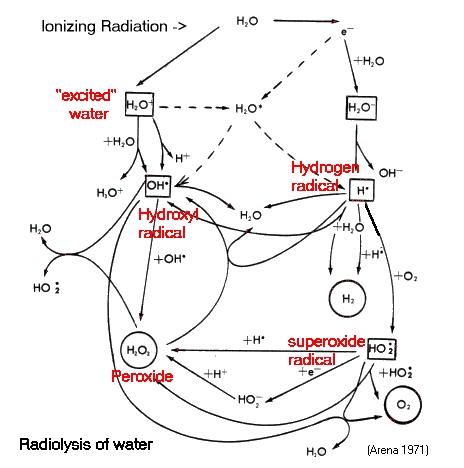
\includegraphics[height=0.6\textheight,width=0.7\textwidth]
      {figures/radiolysis/RadiolysisOfWater.jpg}};
    \small
%    \node[rotate=90] at (0,0){radiolysis of water};
  \end{tikzpicture}
\end{frame}

%%%%%%%%%%%%%%%%%%%%%%%%%%%%%%%%%%%%%%%%%%%%%%%%%%%%%%%%%%%%%%%%%%%%%%
\begin{frame}
  \frametitle{Viability}
  Compare key morphogenetic processes in
  X-rayed \& optical-light viewed embryos. Eg consider balstopore closure 
  \begin{columns}
    \column{0.5\textwidth}
    \begin{tikzpicture}[]
      \def\imh{0.9\textheight}
      \node[anchor=west] at (0,0){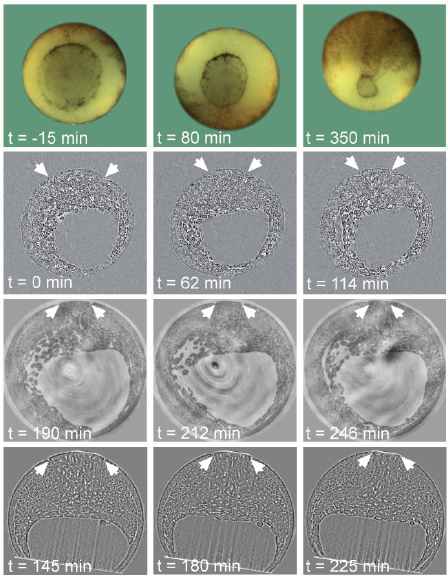
\includegraphics[width=\textwidth]
        {figures/viability/viability.png}};
      \small
      \node[rotate=90,above] at (0,0.25*\imh){optical};
      \node[rotate=90,above] at (0,-0.125*\imh){X-ray};
    \end{tikzpicture}
   \vfill
    \column{0.5\textwidth}
    \begin{itemize}
    \item Rate of balstopore closure
    \end{itemize}
    \begin{tikzpicture}[]
      \def\imh{\textheight}
      \node[anchor=west] at (0,0){
        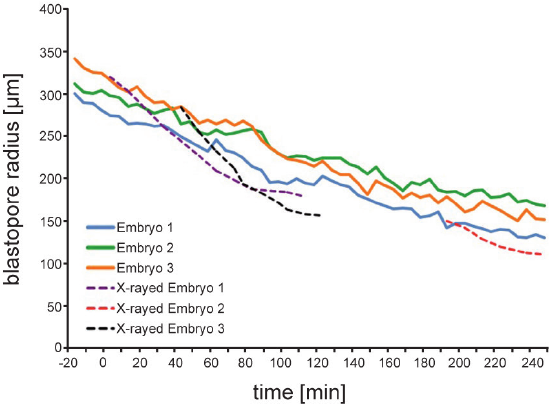
\includegraphics[width=\textwidth, height=0.6\textheight]
        {figures/viability/ClosureRate.png}};
   \end{tikzpicture}
   \vfill
  \end{columns}
\end{frame}

%%%%%%%%%%%%%%%%%%%%%%%%%%%%%%%%%%%%%%%%%%%%%%%%%%%%%%%%%%%%%%%%%%%%%%
\begin{frame}
  \frametitle{Radiolysis-induced degradation of embryo}
    \begin{itemize}
    \item Sagittal sclicing through tomograms at 114 min,
      \SI{124}{min}, \SI{135}{min} after first X-ray scan
    \end{itemize}
    \begin{tikzpicture}
      \node[inner sep=1pt,above] at (0,0){
        \href{run:videos/degradation/NatureDegradation.mp4?autostart&loop}{
          \includegraphics[width=\textwidth,height=0.33\textwidth
          ]{videos/degradation/NatureDegradation.jpg}}};         
      \node[inner sep=1pt,below,align=center] at (-4,0){intact};
      \node[inner sep=1pt,below,align=center] at (0,0){rupture in \\dorsal ectoderm};
      \node[inner sep=1pt,below,align=center] at (4,0){massive outflow \\of cells};
  \end{tikzpicture}
  \begin{flushright}
      \begin{tikzpicture}
      \node[anchor=west] at (0,0){
        \includegraphics[height=0.25\textheight]
        {figures/degradation/xeno_stage_16p5_ruptured.jpg}};
      \node[anchor=east,align=center] at (0,0){optical\\image};
  \end{tikzpicture}
  \end{flushright}
\end{frame}

%%%%%%%%%%%%%%%%%%%%%%%%%%%%%%%%%%%%%%%%%%%%%%%%%%%%%%%%%%%%%%%%%%%%%%
\begin{frame}
  \frametitle{Degradation of embryo}
  Raw projections and corresponding slice through tomograms
  \centering
  \begin{tikzpicture}
    \def\imw{0.75\textwidth}
    \node[above,inner sep=1pt] at (0,0){
        \includegraphics[width=\imw]
        {figures/degradation/EmbryonicDissolution_ProjectionAndVolumeSlices.png}};
      \small
      \node[inner sep=1pt,below,align=center] at (-\imw/3,0){\;intact};
      \node[inner sep=1pt,below,align=center] at (0,0){rupture in \\dorsal ectoderm};
      \node[inner sep=1pt,below,align=center] at (\imw/3,0){massive outflow \\of cells};
  \end{tikzpicture}
  \begin{itemize}
  \item Need for fast/online reconstructions to decide when to terminate scan
  \end{itemize}
\end{frame}

%%%%%%%%%%%%%%%%%%%%%%%%%%%%%%%%%%%%%%%%%%%%%%%%%%%%%%%%%%%%%%%%%%%%%%
%%%%%%%%%%%%%%%%%%%%%%%%%%%%%%%%%%%%%%%%%%%%%%%%%%%%%%%%%%%%%%%%%%%%%%
\subsection{Application}

%%%%%%%%%%%%%%%%%%%%%%%%%%%%%%%%%%%%%%%%%%%%%%%%%%%%%%%%%%%%%%%%%%%%%%
\begin{frame}
  \frametitle{4D in vivo tomography} 
  \begin{columns}[T]
    \column{0.45\textwidth}
    \vfill
    Xenopus gastrulation:
     2-BM@APS, time lapse: \SI{2}{h}, time
    between tomograms: \SI{10}{min}, $\Delta x$=\SI{1}{\micro\metre},
    $E$=\SI{30}{keV}, $\Delta E/E$=\num{e-2}
    \vfill
    \vspace{2cm}
  \begin{tikzpicture}[]
    \def\xx{0.55\textwidth};
    \def\yy{0.61\textwidth};
    \def\imh{0.49\textwidth};
    \small
        % raw proj
         % \node[inner sep=1pt,above] at (\xx,0){
         %   \includegraphics[height=\imh]{figures/xeno-time-lapse/proj-raw}};         
         % \node[inner sep=1pt,below] at (\xx,0){raw projection};
         \node[] at (\xx/2,0){tomographic reconstruction};
         % reco int
         \node[inner sep=1pt,above] at (0,-\yy){
           \includegraphics[height=\imh]{figures/xeno-time-lapse/reco-int}};         
         \node[inner sep=11pt,below] at (0,-\yy){intensity};
         % reco int
         \node[inner sep=1pt,above] at (\xx,-\yy){
           \includegraphics[height=\imh]{figures/xeno-time-lapse/reco-phase}};         
         \node[inner sep=11pt,below] at (\xx,-\yy){phase};

    \end{tikzpicture}
    \column{0.55\textwidth}
    \begin{tikzpicture}
    \small
      % Animated rendering
      \node[inner sep=1pt,above] at (0,0){
        \href{run:videos/xeno-time-lapse/Nature_TomoSlicing.avi?autostart&loop}{
          \includegraphics[width=\textwidth
          ]{videos/xeno-time-lapse/Nature_TomoSlicing.jpg}}};         
      \node[inner sep=1pt,below] at (0,0){Slicing through rendered volume};
      % time-lapse sequence
      \def\yy{0.45\textheight}
      \node[inner sep=1pt,above] at (0,-\yy){
        \href{run:videos/xeno-time-lapse/Nature_TimeLapseSlice.avi?autostart&loop}{
          \includegraphics[width=\textwidth
          ]{videos/xeno-time-lapse/Nature_TimeLapseSlice.jpg}}};         
      \node[inner sep=1pt,below] at (0,-\yy){Time-lapse of reconstructed central slice};
  \end{tikzpicture}
  \end{columns}
\end{frame}


%%%%%%%%%%%%%%%%%%%%%%%%%%%%%%%%%%%%%%%%%%%%%%%%%%%%%%%%%%%%%%%%%%%%%%
\begin{frame}
  \frametitle{Segmentation \& volume analysis}
  What drives the archenteron inflation?
  \vfill
  \begin{tikzpicture}
    \def\imh{0.3\textheight}
    \def\xx{0.5\textwidth}
    \small
    % rotation
    \node[inner sep=1pt,above] at (0,0){
      \href{run:videos/archenteron-inflation/rend-cavities.avi?autostart&loop}{
        \includegraphics[height=\imh]{videos/archenteron-inflation/rend-cavities}}};
    \node[inner sep=1pt,below] at (0,0){Segmented cavities};
    % inflation
    \node[inner sep=1pt,above] at (\xx,0){
      \href{run:videos/archenteron-inflation/infl-arch.avi?autostart&loop}{
        \includegraphics[height=\imh]{videos/archenteron-inflation/infl-arch}}};
    \node[inner sep=1pt,below] at (\xx,0){Inflating archenteron};
  \end{tikzpicture}
  \vfill
  \begin{tikzpicture}[]
    \def\xx{0.2\textwidth}
    \def\imh{0.3\textheight}
    \small
    \node[inner sep=1pt,above] at (0,0){
      \includegraphics[height=\imh]{figures/archenteron-inflation/arch-infl}};         
    \node[inner sep=0pt,below] at (-0.63*\xx,0){Archenteron inflation};
    \node[inner sep=0pt,below] at (1.33*\xx,0){Volume balancing};
  \end{tikzpicture}

  \begin{itemize}
  \item Conclusion: inflation is driven by uptake of external water
  \end{itemize}
\end{frame}

%%%%%%%%%%%%%%%%%%%%%%%%%%%%%%%%%%%%%%%%%%%%%%%%%%%%%%%%%%%%%%%%%%%%%%
\begin{frame}
    \def\xx{0.5\textwidth}
    \def\imh{0.35\textwidth}
    \def\imw{0.8\textwidth}
  \frametitle{Observation of unreported transient structure}
  \begin{itemize}
  \item Confrontation of head \& ventral mesendoderm: formation of a
    transient ridge
    \item Not observable in fixed embryos or explants
  \end{itemize}
  \vfill
  \begin{tikzpicture}[]
    \small
    % im sequence
    \node[inner sep=1pt,above] at (0,0){
      \includegraphics[width=\imw]{figures/transient-ridge/trans-struct-sequ}};         
    \node[inner sep=1pt,below] at (0,0){Time lapse of reconstructed slice};
  \end{tikzpicture}
  \vfill
  \begin{tikzpicture}
    \small
    % embryo cut
    \node[inner sep=1pt,above] at (0,0){
      \includegraphics[height=\imh]{figures/transient-ridge/trans-struct-embryo-cut}};
    \node[inner sep=1pt,below,align=center] at (0,0){Moving contour of \\leading-edge mesendoderm};
    % segmentation
    \node[inner sep=1pt,above] at (\xx,0){
      \href{run:videos/transient-ridge/trans-struct-segm.avi?autostart&loop}{
        \includegraphics[height=\imh]{videos/transient-ridge/trans-struct-segm.jpg}}};
    \node[inner sep=1pt,below] at (\xx,0){Segmented structures};
  \end{tikzpicture}
\end{frame}

%%%%%%%%%%%%%%%%%%%%%%%%%%%%%%%%%%%%%%%%%%%%%%%%%%%%%%%%%%%%%%%%%%%%%%
\begin{frame}
  \frametitle{Optical flow}
  Flow field $\vec{v}$ visualises overall dynamics   
  \begin{tikzpicture}[]
    \def\imw{0.8\textwidth}
    \def\xx{0.4\textwidth}
    \def\yy{0.3\textheight}
    \small
    % rend
    \node[] at (0,0){
      \includegraphics[width=\imw]{figures/optical-flow/rend}};         
    \node[align=right,anchor=east] at (-\xx,0){Rendering of\\ halved embryo};
    % flow
    \node[] at (0,-\yy){
      \includegraphics[width=\imw]{figures/optical-flow/flow}};         
    \node[align=right,anchor=east] at (-\xx,-\yy){Velocity field\\on central slab};
  \end{tikzpicture}
  \begin{itemize}
\small{
  \item Collective cell movements within the gastrula reveals
    % for several morphogenetic processes
    \begin{itemize}
    \item rotation of vegetal endoderm (g: white arrowhead)
    \item involution of  mesendoderm at dorsal \& ventral
      blastopore lip (g: white arrows)
    \item migration of the mesendoderm on the blastocoel roof towards
      the ventral animal pole (g: red arrowhead)
    \end{itemize}}
  \end{itemize}
  \vfill
\end{frame}

%%%%%%%%%%%%%%%%%%%%%%%%%%%%%%%%%%%%%%%%%%%%%%%%%%%%%%%%%%%%%%%%%%%%%%
\begin{frame}
  \frametitle{Differential optical flow} 
   Differential field $g=\abs{\nabla v_x}+\abs{\nabla v_y}+\abs{\nabla v_z}$
  visualises differential cell \& tissue motion$^*$
  \begin{itemize}
  \item Collective vs individual movement
  \item Propulsion mechanisms
  \end{itemize}
  \vfill
  \begin{tikzpicture}[]
    \def\imh{0.4\textheight}
    \def\xx{0.3\textheight}
    \small
    % flow
    \node[inner sep=1pt,above] at (-\xx,0){
      \includegraphics[height=\imh]{figures/optical-flow-diff/flow}};         
    \node[inner sep=1pt,below,align=center] at (-\xx,0){Flow field magnitude $\abs{\vec{v}}$};
    % diff flow
    \node[inner sep=1pt,above] at (\xx,0){
      \includegraphics[height=\imh]{figures/optical-flow-diff/diff-flow}};         
    \node[inner sep=1pt,below,align=center] at (\xx,0){differential field $g$};
  \end{tikzpicture}
  \footnotesize{

    C1: collective motion driven by blastopore closure 

    C2: collective motion driven by involution of dorsal mesendoderm
    plus relative cell motion driven by mediolateral intercalation
    associated with convergent extension}

  I1: crawling of individual cell on blastocoel floor

  \tiny{$^*$non-isotropic definition of $g$
    (L2- instead of L1-norm) also capture directional deviations at
    constant $\abs{\vec{v}}$}
\end{frame}

%%%%%%%%%%%%%%%%%%%%%%%%%%%%%%%%%%%%%%%%%%%%%%%%%%%%%%%%%%%%%%%%%%%%%%
\begin{frame}
  \frametitle{Integrated optical flow}
  \begin{itemize}
  \item Cell tracking via time integration of flow field
  \end{itemize}
  \vfill
  \centering
  \begin{tikzpicture}[]
    \def\imh{0.4\textheight}
    \small
    \node[above] at (0,0){
      \includegraphics[height=\imh]{figures/optical-flow-int/cell-track}};         
    \node[below] at (0,0){Trajectories of cell pairs};
  \end{tikzpicture}
  \vfill
\end{frame}

%%%%%%%%%%%%%%%%%%%%%%%%%%%%%%%%%%%%%%%%%%%%%%%%%%%%%%%%%%%%%%%%%%%%%%
\begin{frame}
  \frametitle{Summary}
  \begin{itemize}
  \item Quasiparticle approach provides a high-resolution phase
    retrieval at large propagation distances and strongly varying
    phases typical for in vivo imaging
  \item Propagation-based, single-distance X-ray phase-contrast
    tomography in combination with optical flow analysis is a useful
    tool for 4D in vivo investigations in developmental biology
  \end{itemize}
\end{frame}

%%%%%%%%%%%%%%%%%%%%%%%%%%%%%%%%%%%%%%%%%%%%%%%%%%%%%%%%%%%%%%%%%%%%%%
\begin{frame}
  \frametitle{Outlook}

  Experiment
  \begin{itemize}
  \item 4th generation synchrotron upgrades (multi-bend achromat
    lattices): drastically enhanced coherence \& brilliance
    $\rightarrow$ enhanced contrast, allows larger $z$
  \item Cone-beam magnification (Kirkpatrick Baez mirrors, ...)
  \item Optimisation of detector system and tomographic acquisition:
    scintillator, microscope, camera
  \item Optimisation of tomographic acquisition: stepping vs
    on-the-fly, fast shutter,
  \item Combine X-ray phase-contrast \& fluorescence
    microscopy or optical projection tomography
  \item Systematic dose studies: dose delay effects, find
    phenomenological function describing dose expression effects, ...
  \end{itemize}

\end{frame}

%%%%%%%%%%%%%%%%%%%%%%%%%%%%%%%%%%%%%%%%%%%%%%%%%%%%%%%%%%%%%%%%%%%%%%
\begin{frame}
  \frametitle{Outlook}

  Theory \& Algorithms
  \begin{itemize}
  \item Adopt quasiparticle approach for transmission electron microscopy 
  \item Variational (iterative) methods from optimisation theory:
    total variation regularisation, sparsity (compressed sensing),
    dictionary learning, neural networks, wavelets/shearlets, ...
  \item Modelling of noise, blurring (scintillator, ...), point spread
    function (MLEM, deconvolution, etc)
  \end{itemize}

  Biology
  \begin{itemize}
  \item Perturbation experiments (wildtype vs morphant embyros): role
    of adhesion molecules, signalling pathways, transcription factors,
    gene regulatory networks, ...
  \item Recent \& upcoming experiments: emigration \& delamination
    processes of neural crest cells as a model for on-set of cancer
    metastasis
  \end{itemize}
\end{frame}

%%%%%%%%%%%%%%%%%%%%%%%%%%%%%%%%%%%%%%%%%%%%%%%%%%%%%%%%%%%%%%%%%%%%%%
\begin{frame}
  \frametitle{Acknowledgement}
  \begin{itemize}
  \item  Karlsruhe Institute of Technology
    \begin{itemize}
      \item Ralf Hofmann
      \item Jubin Kashef
      \item Tilo Baumbach
      \item Alexey Ershov
      \item Venera Weinhard
      \item Daniel Hänschke
    \end{itemize}
  \item Advanced Synchrotron Source
    \begin{itemize}
    \item Xianghui Xao
    \end{itemize}
  \item European Synchrotron Radiation Facility
    \begin{itemize}
    \item Lukas Helfen
    \item Alexander Rack
    \end{itemize}
  \item Northwestern University
    \begin{itemize}
    \item Carole LaBonne
    \item Maneeshi Prasad
    \end{itemize}
  \item KTH - Royal Institute of Technology
    \begin{itemize}
    \item Ozan Öktem
    \end{itemize}
  \end{itemize}
\end{frame}

%%%%%%%%%%%%%%%%%%%%%%%%%%%%%%%%%%%%%%%%%%%%%%%%%%%%%%%%%%%%%%%%%%%%%%
\begin{frame}
\frametitle{Optimal propagation distance}

  Spatio-temporal coherence constrains propagation distances

  \begin{itemize}
  \item Given a transversal coherence length $l_t$ determined by the Van-Zittert
    Zernike theorem and satisfying

    \begin{equation*}
      l_t \ge \frac{\lambda z}{2 \Delta x} = \lambda z \xic \ge \lambda z \abs{\vec{\xi}}
    \end{equation*}
    
    $\lambda$: wave length, $z$: propagation distance, $\Delta x$: pixel size

  \item Given a longitudinal coherence length $l_l$ determined by

    \begin{equation*}
      l_l = \frac{c h}{\Delta E}
    \end{equation*}

    $c$: speed of light, $h$: Planck's constant, $\Delta E$: bandwidth

  \item Window of optimal propagation distances is given by

    \begin{equation*}
      \frac{l_t^2}{2 l_l} \le z \le \frac{d \Delta x}{s}
    \end{equation*}

    $d$: source-sample distance, $s$: source size

  \end{itemize}

\end{frame}


%%%%%%%%%%%%%%%%%%%%%%%%%%%%%%%%%%%%%%%%%%%%%%%%%%%%%%%%%%%%%%%%%%%%%%
\begin{frame}
  \frametitle{Nonlinear phase retrieval: Beyond linear TIE}
  Simulation: Siemens star test pattern, $E=30keV$, $z=0.3m$
  \begin{center}
  \begin{tikzpicture}[]
    \def\imh{0.44\textheight}
    \node[above] at (0,0){
      \includegraphics[height=\imh]{figures/perturb/perturb.png}};         
  \end{tikzpicture}
  \end{center}
  
  $\phi_{0,\mathrm{exact}}$: exact phase map

  $\phi_{0,LO}$: phase map to leading order (Paganin)

  $\phi_{0,NLO}$: phase map to next-to-leading order (Paganin plus
  nonlinear correction)

\end{frame}



%%%%%%%%%%%%%%%%%%%%%%%%%%%%%%%%%%%%%%%%%%%%%%%%%%%%%%%%%%%%%%%%%%%%%%
% \begin{frame}
%   \begin{center}
%     \Large  Thank you for your attention!    
%   \end{center}
% \end{frame}



%%%%%%%%%%%%%%%%%%%%%%%%%%%%%%%%%%%%%%%%%%%%%%%%%%%%%%%%%%%%%%%%%%%%%%
%%%%%%%%%%%%%%%%%%%%%%%%%%%%%%%%%%%%%%%%%%%%%%%%%%%%%%%%%%%%%%%%%%%%%%    
\end{document}

%%%%%%%%%%%%%%%%%%%%%%%%%%%%%%%%%%%%%%%%%%%%%%%%%%%%%%%%%%%%%%%%%%%%%%
% \begin{frame}
%   \frametitle{Data analysis}
%   \begin{columns}
%     %% RIGHT
%     \column{0.5\textwidth}
%     \begin{itemize}
%     \item Visual inspection
%     \end{itemize}
%     \begin{tikzpicture}
%       \def\imw{1.1\textwidth}
%       \node[inner sep=1pt,above] at (0,0){
%         \includegraphics[width=\imw]{figures/analysis-overview/arch-form}};
%       \node[inner sep=1pt,below] at (0,0){
%         \includegraphics[width=\imw]{figures/analysis-overview/trans-ridge}};
%     \end{tikzpicture}
%     \begin{itemize}
%     \item Segmentation
%     \end{itemize}
%       \begin{tikzpicture}
%         \def\imh{0.3\textheight}
%         \node[inner sep=1pt,left] at (0,0){
%           \includegraphics[height=\imh]{figures/analysis-overview/seg-cav}};
%         \node[inner sep=1pt,right] at (0,0){
%           \includegraphics[height=\imh]{figures/analysis-overview/seg-neurula}};
%       \end{tikzpicture}
%     %% MIDDLE
%     \column{0.25\textwidth}
%     % top
%         \vfill
%     \begin{itemize}
%     \item Optical flow: overall dynamics
%     \end{itemize}        
%     \vfill
%     \begin{itemize}
%     \item Differential flow: collective vs individual movement
%     \end{itemize}
%     \vfill
%     \begin{itemize}
%     \item Integrated flow:\\ cell tracking
%     \end{itemize}        
%     %% RIGHT
%     \column{0.25\textwidth}
%     \def\imw{\textwidth}
%     \includegraphics[width=\imw]{figures/analysis-overview/flow}
%     \vfill
%     \includegraphics[width=\imw]{figures/analysis-overview/flow-diff}
%     \vfill
%     \includegraphics[width=\imw]{figures/analysis-overview/flow-int}

%     %   \begin{itemize}
    
%     % \end{itemize}
%     %   \begin{tikzpicture}
%     %     \def\imw{0.5\textwidth}
%     %     \node[inner sep=1pt,above] at (0,0){

%     %   \end{tikzpicture}
%   \end{columns}
% \end{frame}
